% Options for packages loaded elsewhere
\PassOptionsToPackage{unicode,linktoc=all,pdfwindowui,pdfpagemode=FullScreen,pdfpagelayout=TwoPageRight}{hyperref}
\PassOptionsToPackage{hyphens}{url}
\PassOptionsToPackage{dvipsnames,svgnames,x11names}{xcolor}
%
\documentclass[
  9pt,
  letterpaper,
  abstract,
  titlepage]{scrbook}

\usepackage{amsmath,amssymb}
\usepackage{iftex}
\ifPDFTeX
  \usepackage[T1]{fontenc}
  \usepackage[utf8]{inputenc}
  \usepackage{textcomp} % provide euro and other symbols
\else % if luatex or xetex
  \usepackage{unicode-math}
  \defaultfontfeatures{Scale=MatchLowercase}
  \defaultfontfeatures[\rmfamily]{Ligatures=TeX,Scale=1}
\fi
\usepackage{lmodern}
\ifPDFTeX\else  
    % xetex/luatex font selection
\fi
% Use upquote if available, for straight quotes in verbatim environments
\IfFileExists{upquote.sty}{\usepackage{upquote}}{}
\IfFileExists{microtype.sty}{% use microtype if available
  \usepackage[]{microtype}
  \UseMicrotypeSet[protrusion]{basicmath} % disable protrusion for tt fonts
}{}
\usepackage{xcolor}
\usepackage[left=1in,marginparwidth=2.0666666666667in,textwidth=4.1333333333333in,marginparsep=0.3in]{geometry}
\setlength{\emergencystretch}{3em} % prevent overfull lines
\setcounter{secnumdepth}{5}
% Make \paragraph and \subparagraph free-standing
\makeatletter
\ifx\paragraph\undefined\else
  \let\oldparagraph\paragraph
  \renewcommand{\paragraph}{
    \@ifstar
      \xxxParagraphStar
      \xxxParagraphNoStar
  }
  \newcommand{\xxxParagraphStar}[1]{\oldparagraph*{#1}\mbox{}}
  \newcommand{\xxxParagraphNoStar}[1]{\oldparagraph{#1}\mbox{}}
\fi
\ifx\subparagraph\undefined\else
  \let\oldsubparagraph\subparagraph
  \renewcommand{\subparagraph}{
    \@ifstar
      \xxxSubParagraphStar
      \xxxSubParagraphNoStar
  }
  \newcommand{\xxxSubParagraphStar}[1]{\oldsubparagraph*{#1}\mbox{}}
  \newcommand{\xxxSubParagraphNoStar}[1]{\oldsubparagraph{#1}\mbox{}}
\fi
\makeatother
\usepackage{color}
\usepackage{fancyvrb}
\newcommand{\VerbBar}{|}
\newcommand{\VERB}{\Verb[commandchars=\\\{\}]}
\DefineVerbatimEnvironment{Highlighting}{Verbatim}{commandchars=\\\{\}}
% Add ',fontsize=\small' for more characters per line
\usepackage{framed}
\definecolor{shadecolor}{RGB}{241,243,245}
\newenvironment{Shaded}{\begin{snugshade}}{\end{snugshade}}
\newcommand{\AlertTok}[1]{\textcolor[rgb]{0.68,0.00,0.00}{#1}}
\newcommand{\AnnotationTok}[1]{\textcolor[rgb]{0.37,0.37,0.37}{#1}}
\newcommand{\AttributeTok}[1]{\textcolor[rgb]{0.40,0.45,0.13}{#1}}
\newcommand{\BaseNTok}[1]{\textcolor[rgb]{0.68,0.00,0.00}{#1}}
\newcommand{\BuiltInTok}[1]{\textcolor[rgb]{0.00,0.23,0.31}{#1}}
\newcommand{\CharTok}[1]{\textcolor[rgb]{0.13,0.47,0.30}{#1}}
\newcommand{\CommentTok}[1]{\textcolor[rgb]{0.37,0.37,0.37}{#1}}
\newcommand{\CommentVarTok}[1]{\textcolor[rgb]{0.37,0.37,0.37}{\textit{#1}}}
\newcommand{\ConstantTok}[1]{\textcolor[rgb]{0.56,0.35,0.01}{#1}}
\newcommand{\ControlFlowTok}[1]{\textcolor[rgb]{0.00,0.23,0.31}{\textbf{#1}}}
\newcommand{\DataTypeTok}[1]{\textcolor[rgb]{0.68,0.00,0.00}{#1}}
\newcommand{\DecValTok}[1]{\textcolor[rgb]{0.68,0.00,0.00}{#1}}
\newcommand{\DocumentationTok}[1]{\textcolor[rgb]{0.37,0.37,0.37}{\textit{#1}}}
\newcommand{\ErrorTok}[1]{\textcolor[rgb]{0.68,0.00,0.00}{#1}}
\newcommand{\ExtensionTok}[1]{\textcolor[rgb]{0.00,0.23,0.31}{#1}}
\newcommand{\FloatTok}[1]{\textcolor[rgb]{0.68,0.00,0.00}{#1}}
\newcommand{\FunctionTok}[1]{\textcolor[rgb]{0.28,0.35,0.67}{#1}}
\newcommand{\ImportTok}[1]{\textcolor[rgb]{0.00,0.46,0.62}{#1}}
\newcommand{\InformationTok}[1]{\textcolor[rgb]{0.37,0.37,0.37}{#1}}
\newcommand{\KeywordTok}[1]{\textcolor[rgb]{0.00,0.23,0.31}{\textbf{#1}}}
\newcommand{\NormalTok}[1]{\textcolor[rgb]{0.00,0.23,0.31}{#1}}
\newcommand{\OperatorTok}[1]{\textcolor[rgb]{0.37,0.37,0.37}{#1}}
\newcommand{\OtherTok}[1]{\textcolor[rgb]{0.00,0.23,0.31}{#1}}
\newcommand{\PreprocessorTok}[1]{\textcolor[rgb]{0.68,0.00,0.00}{#1}}
\newcommand{\RegionMarkerTok}[1]{\textcolor[rgb]{0.00,0.23,0.31}{#1}}
\newcommand{\SpecialCharTok}[1]{\textcolor[rgb]{0.37,0.37,0.37}{#1}}
\newcommand{\SpecialStringTok}[1]{\textcolor[rgb]{0.13,0.47,0.30}{#1}}
\newcommand{\StringTok}[1]{\textcolor[rgb]{0.13,0.47,0.30}{#1}}
\newcommand{\VariableTok}[1]{\textcolor[rgb]{0.07,0.07,0.07}{#1}}
\newcommand{\VerbatimStringTok}[1]{\textcolor[rgb]{0.13,0.47,0.30}{#1}}
\newcommand{\WarningTok}[1]{\textcolor[rgb]{0.37,0.37,0.37}{\textit{#1}}}

\providecommand{\tightlist}{%
  \setlength{\itemsep}{0pt}\setlength{\parskip}{0pt}}\usepackage{longtable,booktabs,array}
\usepackage{calc} % for calculating minipage widths
% Correct order of tables after \paragraph or \subparagraph
\usepackage{etoolbox}
\makeatletter
\patchcmd\longtable{\par}{\if@noskipsec\mbox{}\fi\par}{}{}
\makeatother
% Allow footnotes in longtable head/foot
\IfFileExists{footnotehyper.sty}{\usepackage{footnotehyper}}{\usepackage{footnote}}
\makesavenoteenv{longtable}
\usepackage{graphicx}
\makeatletter
\newsavebox\pandoc@box
\newcommand*\pandocbounded[1]{% scales image to fit in text height/width
  \sbox\pandoc@box{#1}%
  \Gscale@div\@tempa{\textheight}{\dimexpr\ht\pandoc@box+\dp\pandoc@box\relax}%
  \Gscale@div\@tempb{\linewidth}{\wd\pandoc@box}%
  \ifdim\@tempb\p@<\@tempa\p@\let\@tempa\@tempb\fi% select the smaller of both
  \ifdim\@tempa\p@<\p@\scalebox{\@tempa}{\usebox\pandoc@box}%
  \else\usebox{\pandoc@box}%
  \fi%
}
% Set default figure placement to htbp
\def\fps@figure{htbp}
\makeatother

% Package imports

\usepackage[english]{babel}
\usepackage[outercaption, ragged]{sidecap}
\usepackage{adjustbox}
\usepackage{afterpage}
\usepackage{array}
\usepackage{atbegshi} % Package to insert content at the beginning
\usepackage{caption}
\captionsetup[table]{belowskip=5pt}
\usepackage{etoolbox}% For redefining footnotes
\usepackage{fancyhdr}
\usepackage{fontspec}
\usepackage{geometry}
\usepackage{graphicx}
\usepackage{float}
\usepackage{hyperref}
\usepackage{ifthen}
\usepackage{longtable}
\usepackage{marginfix} % Fixes the issue of margin notes being cut off
\usepackage{marginnote}
\usepackage{mathptmx}
\usepackage{newpxtext} % Palatino-like font
\usepackage{ragged2e}
\usepackage{sidenotes}
\usepackage{titlesec}
\usepackage{tocloft}
\usepackage{xcolor}
\usepackage{changepage}
\usepackage{emptypage}
\usepackage[all]{nowidow}
\usepackage{amsmath}
\usepackage{enumitem}

\def\tightlist{}
\setlist{itemsep=1pt, parsep=1pt, topsep=0pt,after={\vspace{0.3\baselineskip}}}
\let\tightlist\relax

\usepackage{listings}
\lstset{
breaklines=true,  % wraping
breakatwhitespace=true,  
basicstyle=\ttfamily,  
frame=none,   
keepspaces=true,  
showspaces=false,   
showtabs=false,  
columns=flexible,
belowskip=0pt,
aboveskip=0pt
}
% \geometry{
%   paperwidth=7.5in,
%   paperheight=9.25in,
%   top=1in,
%   bottom=1in,
%   inner=1in,
%   outer=2.25in,
%   footskip=30pt,
%   marginparwidth=1.5in,
%   twoside
\geometry{
 paperwidth=7.5in,
 paperheight=9.25in,
 margin=1in,
 footskip=30pt
}


% Define the Crimson color
\definecolor{crimson}{HTML}{A51C30}

% Redefine \sidenote to include a custom minimalist styled box with a vertical bar
\renewcommand{\thefootnote}{\textcolor{crimson}{\arabic{footnote}}}

\makeatletter
\renewcommand\chapter{\clearpage\global\@topnum\z@
\@afterindentfalse \secdef\@chapter\@schapter}
\makeatother

% Save the old \sidenote command (only if it exists)
\makeatletter
\@ifundefined{oldsidenote}{
  \let\oldsidenote\sidenote%
}{}
\makeatother

% Redefine \sidenote
\renewcommand{\sidenote}[1]{%
  \oldsidenote{%
    \noindent
    \color{crimson!100} % Set the color for the vertical line
    \raisebox{0em}{% Raise the vertical line to align with the number
      \rule{0.5pt}{1.5em} % Thin vertical line with fixed height
    }
    \hspace{0.3em} % Spacing between the line and the sidenote text
    \color{black} % Reset color for sidenote text
    {\footnotesize #1} % Sidenote text in smaller font size
  }
}

% Custom LaTeX commands and definitions
\newcommand{\centeredimage}[2][0.9\textwidth]{%
  \begin{center}
    \includegraphics[width=#1]{#2}
  \end{center}
}

% Redefine the figure environment (fixes the bug where even page captions don't show, odd I know!)
\makeatletter
\let\oldfigure\figure%
\let\endoldfigure\endfigure%
\renewenvironment{figure}[1][htbp]{%
  \oldfigure[#1]%
}{%
  \endoldfigure%
}
\makeatother

\babelprovide[import]{czech}

\patchcmd{\chapter}{\thispagestyle{plain}}{\thispagestyle{fancy}}{}{}

% Page style settings
\pagestyle{fancy}
\fancyhf{}
\fancyhead[LE]{\small\color{crimson}\nouppercase{\rightmark}}
\fancyhead[RO]{\color{crimson}\thepage}
\fancyhead[LO]{\small\color{crimson}\nouppercase{\leftmark}}
\fancyhead[RE]{\color{crimson}\thepage}
\renewcommand{\headrulewidth}{0.4pt}
\renewcommand{\footrulewidth}{0pt}
\fancypagestyle{plain}{
  \fancyhf{}
  \fancyfoot[C]{\color{crimson}\thepage}
  \renewcommand{\headrulewidth}{0pt}
  \renewcommand{\footrulewidth}{0pt}
}

% KOMA-Script adjustments
\addtokomafont{disposition}{\rmfamily\color{crimson}}
\addtokomafont{chapter}{\color{crimson}}
\addtokomafont{section}{\color{crimson}}
\addtokomafont{subsection}{\color{crimson}}

\newenvironment{abstract}{
  \chapter*{\abstractname}
  \addcontentsline{toc}{chapter}{\abstractname}
  \small
}{
  \clearpage 
}

% \hypersetup{
%   linkcolor=crimson,
%   citecolor=crimson,
%   urlcolor=crimson,
%   pdfpagelayout=TwoPageRight, % This sets the layout to two-page mode with the first page alone
%   pdfstartview=Fit % This sets the initial zoom to fit the page
% }
\hypersetup{
 linkcolor=crimson,
 citecolor=crimson,
 urlcolor=crimson,
 pdfpagelayout=OneColumn,
 pdfstartview=Fit
}

\renewcommand{\part}[1]{%
    \chapter*{#1} % Render the part title without a number
    \addcontentsline{toc}{part}{#1} % Add to TOC without numbering
}

% % Redefine \part to do nothing
% \renewcommand{\part}[1]{%
%     \typeout{Skipping \detokenize{#1}}% Print message in the log file
% }

% % Ensure \partname is defined, just in case it's referenced elsewhere
% \renewcommand{\partname}{}

% % Redefine \part (if you want to apply the Crimson color here)
% \titleformat{\part}[display]
%   {\normalfont\Huge\bfseries\color{crimson}} % Set the color to crimson
%   {\partname~\thepart}
%   {0pt}
%   {\Huge}
%   [\vspace{20pt}]

% Redefine \section
\titleformat{\section}
  {\normalfont\Large\bfseries\color{crimson}\raggedright} % Set the color to crimson
  {\thesection}
  {0.5em}
  {}
  \titlespacing*{\section}{0pc}{14pt plus 4pt minus 4pt}{6pt plus 2pt minus 2pt}[0pc]

% Redefine \subsection
\titleformat{\subsection}
  {\normalfont\large\bfseries\color{crimson}\raggedright} % Set the color to crimson
  {\thesubsection}
  {0.5em}
  {}
\titlespacing*{\subsection}{0pc}{12pt plus 4pt minus 4pt}{5pt plus 1pt minus 2pt}[0pc] 

% Redefine \subsubsection
\titleformat{\subsubsection}
  {\normalfont\normalsize\bfseries\color{crimson}\raggedright} % Set the color to crimson
  {\thesubsubsection}
  {0.5em}
  {}
\titlespacing*{\subsubsection}{0pc}{12pt plus 4pt minus 4pt}{5pt plus 1pt minus 2pt}[0pc]  

% Redefine \paragraph (if you want to apply the Crimson color here)
\titleformat{\paragraph}[runin]
  {\normalfont\normalsize\bfseries\color{crimson}} % Set the color to crimson
  {\theparagraph}
  {0.5em}
  {}
  [\textbf{.}]

% Redefine \subparagraph (if you want to apply the Crimson color here)
\titleformat{\subparagraph}[runin]
  {\normalfont\normalsize\itshape\color{crimson}}% Set the color to crimson
  {\thesubparagraph}
  {0.5em}
  {}
  [\textbf{.}]

% Customize Chapter title format
\titleformat{\chapter}[display]
  {\normalfont\huge\bfseries\color{crimson}} % Apply the crimson color
  {\chaptername\ \thechapter} % Prefix "Chapter X"
  {20pt} % Space between number and title
  {\Huge} % Format the title itself
  []

% Ensure that \chaptername is set to "Chapter"
\renewcommand{\chaptername}{Chapter}
\setcounter{tocdepth}{2}
\setlength{\cftsecnumwidth}{2.75em} % Adjust width for section numbers
\setlength{\cftsubsecnumwidth}{3.25em} % Adjust width for subsection numbers
\setlength{\cftsubsubsecnumwidth}{4em} % Adjust width for subsubsection numbers

% Page numbering setup
\makeatletter
% Store whether we've seen the first of each type
\newif\if@firstnumbered%
\@firstnumberedtrue%
\newif\if@firstunnumbered%
\@firstunnumberedtrue%

% Store the page numbers
\newcounter{lastRomanPage}
\setcounter{lastRomanPage}{1}

% Initial setup for front matter
\AtBeginDocument{
  \pagenumbering{roman}
  \renewcommand{\thepage}{\roman{page}}
}

% Modify chapter to handle page numbering
\let\old@chapter\chapter%
\renewcommand{\chapter}{%
  \@ifstar{\unnumbered@chapter}{\numbered@chapter}%
}

% Handle numbered chapters
\newcommand{\numbered@chapter}[1]{%
  \if@firstnumbered%
    \cleardoublepage%
    \setcounter{lastRomanPage}{\value{page}}%
    \pagenumbering{arabic}%
    \@firstnumberedfalse%
  \else
    \setcounter{page}{\value{page}}%
  \fi
  \old@chapter{#1}%
}

% Handle unnumbered chapters - only switch on actual chapter changes
\newcommand{\unnumbered@chapter}[1]{%
  \if@firstunnumbered%
    \clearpage
    \setcounter{lastRomanPage}{\value{page}}%
    \pagenumbering{roman}%
    \@firstunnumberedfalse%
  \fi
  \old@chapter*{#1}%
}
\makeatother

\AtBeginEnvironment{longtable}{\scriptsize} % Adjust to \footnotesize or \scriptsize if needed
\makeatletter
\@ifpackageloaded{float}{}{\usepackage{float}}
\floatstyle{plain}
\@ifundefined{c@chapter}{\newfloat{lab}{h}{lolabq}}{\newfloat{lab}{h}{lolabq}[chapter]}
\floatname{lab}{Lab}
\newcommand*\listoflabs{\listof{lab}{List of Labs}}
\makeatother
\makeatletter
\@ifpackageloaded{float}{}{\usepackage{float}}
\floatstyle{plain}
\@ifundefined{c@chapter}{\newfloat{exr}{h}{loexr}}{\newfloat{exr}{h}{loexr}[chapter]}
\floatname{exr}{Exercise}
\newcommand*\listofexrs{\listof{exr}{List of Exercises}}
\makeatother
\makeatletter
\@ifpackageloaded{float}{}{\usepackage{float}}
\floatstyle{plain}
\@ifundefined{c@chapter}{\newfloat{vid}{h}{lovid}}{\newfloat{vid}{h}{lovid}[chapter]}
\floatname{vid}{Video}
\newcommand*\listofvids{\listof{vid}{List of Videos}}
\makeatother
\makeatletter
\@ifpackageloaded{tcolorbox}{}{\usepackage[skins,breakable]{tcolorbox}}
\@ifpackageloaded{fontawesome5}{}{\usepackage{fontawesome5}}
\definecolor{quarto-callout-color}{HTML}{909090}
\definecolor{quarto-callout-note-color}{HTML}{0758E5}
\definecolor{quarto-callout-important-color}{HTML}{CC1914}
\definecolor{quarto-callout-warning-color}{HTML}{EB9113}
\definecolor{quarto-callout-tip-color}{HTML}{00A047}
\definecolor{quarto-callout-caution-color}{HTML}{FC5300}
\definecolor{quarto-callout-color-frame}{HTML}{acacac}
\definecolor{quarto-callout-note-color-frame}{HTML}{4582ec}
\definecolor{quarto-callout-important-color-frame}{HTML}{d9534f}
\definecolor{quarto-callout-warning-color-frame}{HTML}{f0ad4e}
\definecolor{quarto-callout-tip-color-frame}{HTML}{02b875}
\definecolor{quarto-callout-caution-color-frame}{HTML}{fd7e14}
\makeatother
\makeatletter
\@ifpackageloaded{bookmark}{}{\usepackage{bookmark}}
\makeatother
\makeatletter
\@ifpackageloaded{caption}{}{\usepackage{caption}}
\AtBeginDocument{%
\ifdefined\contentsname
  \renewcommand*\contentsname{Table of contents}
\else
  \newcommand\contentsname{Table of contents}
\fi
\ifdefined\listfigurename
  \renewcommand*\listfigurename{List of Figures}
\else
  \newcommand\listfigurename{List of Figures}
\fi
\ifdefined\listtablename
  \renewcommand*\listtablename{List of Tables}
\else
  \newcommand\listtablename{List of Tables}
\fi
\ifdefined\figurename
  \renewcommand*\figurename{Figure}
\else
  \newcommand\figurename{Figure}
\fi
\ifdefined\tablename
  \renewcommand*\tablename{Table}
\else
  \newcommand\tablename{Table}
\fi
}
\@ifpackageloaded{float}{}{\usepackage{float}}
\floatstyle{ruled}
\@ifundefined{c@chapter}{\newfloat{codelisting}{h}{lop}}{\newfloat{codelisting}{h}{lop}[chapter]}
\floatname{codelisting}{Listing}
\newcommand*\listoflistings{\listof{codelisting}{List of Listings}}
\makeatother
\makeatletter
\makeatother
\makeatletter
\@ifpackageloaded{caption}{}{\usepackage{caption}}
\@ifpackageloaded{subcaption}{}{\usepackage{subcaption}}
\makeatother
\makeatletter
\@ifpackageloaded{sidenotes}{}{\usepackage{sidenotes}}
\@ifpackageloaded{marginnote}{}{\usepackage{marginnote}}
\makeatother

\usepackage{hyphenat}
\usepackage{ifthen}
\usepackage{calc}
\usepackage{calculator}



\usepackage{graphicx}
\usepackage{geometry}
\usepackage{afterpage}
\usepackage{tikz}
\usetikzlibrary{calc}
\usetikzlibrary{fadings}
\usepackage[pagecolor=none]{pagecolor}


% Set the titlepage font families







% Set the coverpage font families


\usepackage{bookmark}

\IfFileExists{xurl.sty}{\usepackage{xurl}}{} % add URL line breaks if available
\urlstyle{same} % disable monospaced font for URLs
\hypersetup{
  pdftitle={Embedded Systems Design},
  colorlinks=true,
  linkcolor={Maroon},
  filecolor={Maroon},
  citecolor={Blue},
  urlcolor={Blue},
  pdfcreator={LaTeX via pandoc}}


\title{Embedded Systems Design}
\usepackage{etoolbox}
\makeatletter
\providecommand{\subtitle}[1]{% add subtitle to \maketitle
  \apptocmd{\@title}{\par {\large #1 \par}}{}{}
}
\makeatother
\subtitle{Utilizing the Silicon Labs EFR32XG24 BLE Microcontroller}
\author{}
\date{January 23, 2025}

\begin{document}
%%%%% begin titlepage extension code

  \begin{frontmatter}

\begin{titlepage}
% This is a combination of Pandoc templating and LaTeX
% Pandoc templating https://pandoc.org/MANUAL.html#templates
% See the README for help

\thispagestyle{empty}

\newgeometry{top=-100in}

% Page color

\newcommand{\coverauthorstyle}[1]{{\fontsize{20}{24.0}\selectfont
{#1}}}

\begin{tikzpicture}[remember picture, overlay, inner sep=0pt, outer sep=0pt]

\tikzfading[name=fadeout, inner color=transparent!0,outer color=transparent!100]
\tikzfading[name=fadein, inner color=transparent!100,outer color=transparent!0]
\node[anchor=south west, rotate=0, opacity=1] at ($(current page.south west)+(0.0, 7)$) {
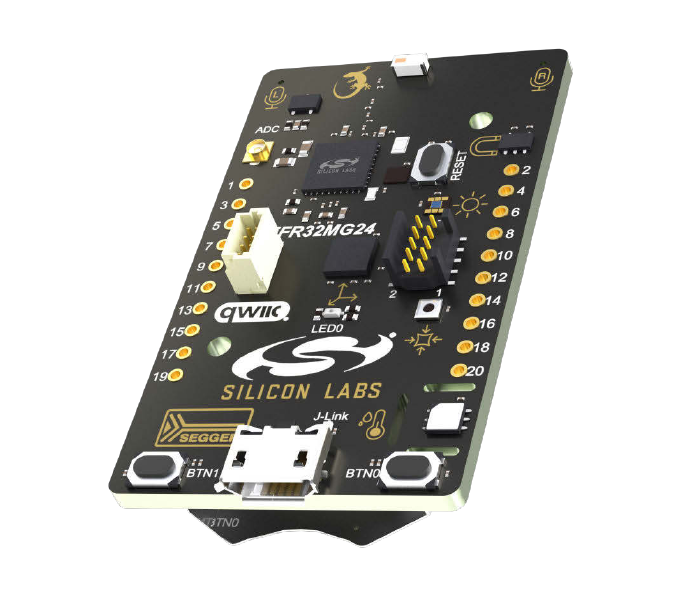
\includegraphics[width=\paperwidth, keepaspectratio]{cover-image-transparent.png}};

% Title
\newcommand{\titlelocationleft}{0.075\paperwidth}
\newcommand{\titlelocationbottom}{0.375\paperwidth}
\newcommand{\titlealign}{left}

\begin{scope}{%
\fontsize{38}{45.6}\selectfont
\node[anchor=north
west, align=left, rotate=0] (Title1) at ($(current page.south west)+(\titlelocationleft,\titlelocationbottom)$)  [text width = 0.9\paperwidth]  {{\nohyphens{Embedded
Systems Design}}};
}
\end{scope}

% Author
\newcommand{\authorlocationleft}{7in}
\newcommand{\authorlocationbottom}{0.15\paperwidth}
\newcommand{\authoralign}{right}

\begin{scope}
{%
\fontsize{20}{24.0}\selectfont
\node[anchor=north
east, align=right, rotate=0] (Author1) at ($(current page.south west)+(\authorlocationleft,\authorlocationbottom)$)  [text width = 6in]  {\coverauthorstyle{Masudul\\Imtiaz\\}};
}
\end{scope}

\end{tikzpicture}
\clearpage
\restoregeometry
%%% TITLE PAGE START

% Set up alignment commands
%Page
\newcommand{\titlepagepagealign}{
\ifthenelse{\equal{left}{right}}{\raggedleft}{}
\ifthenelse{\equal{left}{center}}{\centering}{}
\ifthenelse{\equal{left}{left}}{\raggedright}{}
}


\newcommand{\titleandsubtitle}{
% Title and subtitle
{{\huge{\bfseries{\nohyphens{Embedded Systems Design}}}}\par
}%

\vspace{\betweentitlesubtitle}
{
{\large{\textit{\nohyphens{Utilizing the Silicon Labs EFR32XG24 BLE
Microcontroller}}}}\par
}}
\newcommand{\titlepagetitleblock}{
\titleandsubtitle
}

\newcommand{\authorstyle}[1]{{\large{#1}}}

\newcommand{\affiliationstyle}[1]{{\large{#1}}}

\newcommand{\titlepageauthorblock}{
{\authorstyle{}}}

\newcommand{\titlepageaffiliationblock}{
\hangindent=1em
\hangafter=1
{\affiliationstyle{


\vspace{1\baselineskip} 
}}
}
\newcommand{\headerstyled}{%
{}
}
\newcommand{\footerstyled}{%
{\large{}}
}
\newcommand{\datestyled}{%
{January 23, 2025}
}


\newcommand{\titlepageheaderblock}{\headerstyled}

\newcommand{\titlepagefooterblock}{
\footerstyled
}

\newcommand{\titlepagedateblock}{
\datestyled
}

%set up blocks so user can specify order
\newcommand{\titleblock}{\newlength{\betweentitlesubtitle}
\setlength{\betweentitlesubtitle}{0.05\textheight}
{

{\titlepagetitleblock}
}

\vspace{4\baselineskip}
}

\newcommand{\authorblock}{}

\newcommand{\affiliationblock}{}

\newcommand{\logoblock}{}

\newcommand{\footerblock}{}

\newcommand{\dateblock}{{\titlepagedateblock}

\vspace{0pt}
}

\newcommand{\headerblock}{}

\thispagestyle{empty} % no page numbers on titlepages


\newcommand{\vrulecode}{\textcolor{black}{\rule{\vrulewidth}{\textheight}}}
\newlength{\vrulewidth}
\setlength{\vrulewidth}{2pt}
\newlength{\B}
\setlength{\B}{\ifdim\vrulewidth > 0pt 0.05\textwidth\else 0pt\fi}
\newlength{\minipagewidth}
\ifthenelse{\equal{left}{left} \OR \equal{left}{right} }
{% True case
\setlength{\minipagewidth}{\textwidth - \vrulewidth - \B - 0.1\textwidth}
}{
\setlength{\minipagewidth}{\textwidth - 2\vrulewidth - 2\B - 0.1\textwidth}
}
\ifthenelse{\equal{left}{left} \OR \equal{left}{leftright}}
{% True case
\raggedleft % needed for the minipage to work
\vrulecode
\hspace{\B}
}{%
\raggedright % else it is right only and width is not 0
}
% [position of box][box height][inner position]{width}
% [s] means stretch out vertically; assuming there is a vfill
\begin{minipage}[b][\textheight][s]{\minipagewidth}
\titlepagepagealign
\titleblock

Masudul Imtiaz, PhD

Sigmond Kukla

Aaron Storey, MSAI

\& TA's of EE260

\vspace{0.75cm}

Coulson School of Engineering and Applied Sciences

Clarkson University

\vfill
\par

\end{minipage}\ifthenelse{\equal{left}{right} \OR \equal{left}{leftright} }{
\hspace{\B}
\vrulecode}{}
\clearpage
%%% TITLE PAGE END
\end{titlepage}
\setcounter{page}{1}
\end{frontmatter}

%%%%% end titlepage extension code

\renewcommand*\contentsname{Table of contents}
{
\hypersetup{linkcolor=}
\setcounter{tocdepth}{2}
\tableofcontents
}

\mainmatter
\bookmarksetup{startatroot}

\chapter*{Preface}\label{preface}
\addcontentsline{toc}{chapter}{Preface}

\markboth{Preface}{Preface}

\section*{Welcome}\label{welcome}
\addcontentsline{toc}{section}{Welcome}

\markright{Welcome}

Welcome to the \textbf{``System Design with Silicon Lab EFR32XG24 BLE
Microcontroller''}. This book is designed to guide you through the
process of programming, building applications, and integrating machine
learning with the EFR32XG24 BLE Microcontroller. Whether you're an
engineering student or a seasoned professional, this book offers
hands-on examples to make advanced concepts accessible.

You'll learn how to: - Program the EFR32XG24 microcontroller using C. -
Design and implement embedded systems applications. - Apply machine
learning techniques to solve real-world problems. - Explore gesture
recognition, anomaly detection, and audio-based ML solutions.

The book balances theory with practice, empowering readers to develop
embedded systems that are robust, efficient, and intelligent.

If you're interested in broader programming concepts or other machine
learning platforms, we encourage you to explore additional resources and
apply your learning across domains.

\begin{tcolorbox}[enhanced jigsaw, opacityback=0, leftrule=.75mm, left=2mm, breakable, bottomrule=.15mm, colback=white, arc=.35mm, toprule=.15mm, rightrule=.15mm, colframe=quarto-callout-note-color-frame]
\begin{minipage}[t]{5.5mm}
\textcolor{quarto-callout-note-color}{\faInfo}
\end{minipage}%
\begin{minipage}[t]{\textwidth - 5.5mm}

This book was originally developed as part of the EE260 and EE513
courses at Clarkson University. The Quarto-based version serves as an
example of modern technical publishing and open access education.

\end{minipage}%
\end{tcolorbox}

\section*{License}\label{license}
\addcontentsline{toc}{section}{License}

\markright{License}

This book is \textbf{free to use} under the
\href{https://creativecommons.org/licenses/by-nc-sa/4.0/}{Creative
Commons Attribution-NonCommercial-ShareAlike 4.0 International} License.
You are welcome to share, adapt, and use the material for educational
purposes, as long as proper attribution is given and no commercial use
is made.

If you'd like to support the project or contribute, you can report
issues or submit pull requests at
\href{https://github.com/clarkson-edge/ee513_book}{github.com/clarkson-edge/ee513\_book}.
Thank you for helping improve this resource for the community.

\part{Embedded Systems Design}

\chapter{Introduction}\label{introduction}

This chapter introduces the essential concepts of embedded systems and
highlights the growing significance of BLE technology in modern designs.
It emphasizes the role of microcontrollers, particularly the Silicon
Labs EFR32XG24, in enabling efficient, low-power wireless communication
for IoT applications. Whether you are a student starting your embedded
systems journey or an engineer aiming to enhance your design skills,
this booklet will serve as a valuable resource to build innovative and
efficient BLE-enabled embedded solutions.

\section{Overview}\label{overview}

Embedded systems are specialized computing systems that are designed to
perform dedicated functions or tasks within a larger mechanical or
electrical system. Unlike general-purpose computers, embedded systems
are optimized for specific applications, balancing constraints such as
power consumption, real-time performance, and cost efficiency. They are
integral to a wide range of applications, including consumer
electronics, automotive systems, medical devices, industrial automation,
and smart home technologies.

At the core of most embedded systems lies a microcontroller, a compact
integrated circuit that combines a processor, memory, and input/output
peripherals on a single chip. Microcontrollers are the brain of embedded
systems, executing pre-programmed instructions to manage sensors,
actuators, and communication modules. Their efficiency, reliability, and
low power consumption make them ideal for embedded applications.

In recent years, the demand for wireless communication in embedded
systems has surged, driven by the growth of the Internet of Things
(IoT). Among the various wireless protocols, Bluetooth Low Energy (BLE)
has emerged as a key technology for low-power, short-range
communication. BLE enables devices to transmit small amounts of data
with minimal energy consumption, making it ideal for battery-operated
applications such as fitness trackers, smart home devices, and health
monitoring systems.

The Silicon Labs EFR32XG24 series is one of the most advanced BLE
microcontrollers available in Q4 of 2024. Built on the ARM Cortex-M33
core, it offers a powerful blend of performance, energy efficiency, and
wireless connectivity. It is equipped with a robust BLE stack, extensive
peripherals, and advanced security features, making it a preferred
choice for designing sophisticated embedded systems.

This textbook, \emph{System Design with Silicon Lab EFR32XG24 BLE
Microcontroller}, is intended to provide a guide for students and
engineers to understand and design embedded systems using the EFR32xG24
Dev Kit. The book covers both theoretical concepts and hands-on
practical implementations, ensuring readers gain a deep understanding of
embedded system design and BLE communication protocols.

Throughout this book, readers will learn:

\begin{itemize}
\item
  The fundamentals of embedded systems and microcontroller architecture.
\item
  Key features and capabilities of the EFR32XG24 BLE microcontroller.
\item
  Practical techniques for programming and debugging embedded systems.
\item
  BLE communication protocols and integration with IoT applications.
\item
  Real-world case studies and projects demonstrating system design
  principles.
\end{itemize}

\section{Real-World Applications of Embedded
Systems}\label{real-world-applications-of-embedded-systems}

Embedded systems are deeply integrated into modern life, serving as the
backbone for countless devices and technologies. They are designed to
execute dedicated functions efficiently while operating under
constraints such as power consumption, memory limitations, and cost.
Examples of embedded systems can be observed in both everyday objects
and complex industrial applications, showcasing their versatility and
importance in modern engineering.

One prominent example is the automotive industry, where embedded systems
play a critical role in ensuring safety, efficiency, and advanced
functionalities. Anti-lock Braking Systems (ABS) use embedded
controllers to regulate brake pressure, preventing skidding on slippery
roads and enhancing vehicle stability. Similarly, adaptive cruise
control systems utilize embedded microcontrollers to monitor vehicle
speed and distance through RADAR or LIDAR sensors, enabling intelligent
speed adjustments. Another safety-critical application is the airbag
control system, which relies on real-time sensor data to trigger airbag
deployment within milliseconds during a collision.

In industrial automation, embedded systems are central to the operation
of robotic arms, conveyor belts, and assembly lines. These systems
handle precise sequencing, closed-loop control, and real-time signal
processing to maintain efficiency and safety. For example, industrial
robots are programmed to carry out repetitive tasks such as welding,
painting, and packaging, each controlled by embedded microcontrollers to
ensure accuracy and reliability.

Consumer electronics also heavily rely on embedded systems. Devices such
as programmable engineering calculators, automated teller machines
(ATMs), and smart home appliances incorporate microcontrollers to
perform specific tasks seamlessly. Modern washing machines, for
instance, utilize embedded controllers to monitor water levels, manage
wash cycles, and adjust spin speeds dynamically. Similarly, ATMs use
embedded microcontrollers to process transactions securely while
managing input and output operations.

BLE microcontrollers have further extended the capabilities of embedded
systems by enabling low-power wireless communication. BLE technology is
particularly advantageous in battery-operated devices like fitness
trackers, smart home sensors, and medical monitoring equipment. These
microcontrollers facilitate energy-efficient data transmission, allowing
devices to remain functional for extended periods without frequent
battery replacements.

\section{Overview of EFR32MG24
Microcontroller}\label{overview-of-efr32mg24-microcontroller}

The EFR32MG24 microcontroller, part of Silicon Labs' Wireless Gecko
series, is specifically designed to address the growing demand for
energy-efficient and high-performance wireless communication in embedded
systems. Built on the ARM Cortex-\textbf{M33} core, it operates at a
maximum frequency of \textbf{78} MHz, delivering sufficient
computational power for real-time applications while maintaining energy
efficiency. The microcontroller integrates advanced hardware security
features, including a hardware cryptographic accelerator and Secure
Boot, ensuring robust protection against cyber threats. It supports
multiple wireless protocols, with a primary focus on BLE 5.3, enabling
reliable, low-power, short-range communication. The integrated radio
transceiver offers industry-leading sensitivity and output power,
ensuring stable connectivity even in challenging environments.

The EFR32MG24 is equipped with a range of analog and digital
peripherals, including ADCs, DACs, timers, UART, SPI, and I2C
interfaces, providing flexible options for sensor integration and
peripheral control. Its low-power modes, combined with energy-saving
peripherals and Sleep Timer capabilities, make it highly suitable for
battery-operated devices such as IoT sensor nodes, wearable electronics,
and smart home devices. This also features an on-chip AI/ML hardware
accelerator, enabling edge-computing capabilities for tasks like sensor
data analysis and anomaly detection. Hence, this microcontroller,
available in the xG24-DK2601B Development Kit, is chosen for this book.

\chapter{\texorpdfstring{\textbf{Programming Embedded Systems with
C}}{Programming Embedded Systems with C}}\label{programming-embedded-systems-with-c}

Embedded systems rely heavily on the C programming language due to its
efficiency, low-level hardware access, and portability across different
microcontroller architectures. This chapter explores the foundational
concepts of C programming in the context of embedded systems, with a
focus on optimizing performance, managing data types, and effectively
using hardware resources. By mastering these fundamental concepts,
readers will be better prepared to develop efficient and reliable
embedded systems using the Silicon Labs EFR32XG24 BLE microcontroller.

\section{Simplicity Studio IDE for Silicon Labs EFR32XG24
Microcontroller}\label{simplicity-studio-ide-for-silicon-labs-efr32xg24-microcontroller}

Simplicity Studio is the official Integrated Development Environment
(IDE) provided by Silicon Labs for embedded development with their
microcontrollers, including the EFR32XG24 BLE microcontroller to be
covered in this textbook. It is a feature-rich platform designed to
streamline the development process, offering a library of example
projects, application templates, and related tools for writing,
debugging, profiling, and deploying firmware applications efficiently.
It integrates multiple tools into one unified interface:

\begin{itemize}
\item
  \textbf{Project Management:} Create, organize, and manage embedded
  projects.
\item
  \textbf{Device Configuration:} Configure peripheral modules and
  optimize hardware settings.
\item
  \textbf{Debugging Tools:} Real-time debugging with SEGGER J-Link
  integration.
\item
  \textbf{Energy Profiler:} Monitor and optimize power consumption of
  embedded applications.
\item
  \textbf{Wireless Network Analyzer:} Analyze wireless traffic and
  optimize communication protocols.
\end{itemize}

Simplicity Studio supports a range of compilers tailored for embedded
systems:

\begin{itemize}
\item
  \textbf{GCC (GNU Compiler Collection):} Open-source compiler widely
  used in embedded systems.
\item
  \textbf{IAR Embedded Workbench Compiler:} Commercial compiler known
  for its optimization capabilities.
\item
  \textbf{Keil ARM Compiler (ARMCC):} Industry-standard compiler for ARM
  Cortex-M series microcontrollers.
\end{itemize}

For the EFR32XG24 microcontroller, \textbf{\emph{GCC}} is the default
compiler bundled with Simplicity Studio, offering robust optimization
and compatibility with ARM Cortex-M33 cores.

\subsection{Development Workflow in Simplicity
Studio}\label{development-workflow-in-simplicity-studio}

The typical workflow when using Simplicity Studio for EFR32XG24
development involves:

\begin{enumerate}
\def\labelenumi{\arabic{enumi}.}
\item
  \textbf{Device Selection:} Select the target microcontroller
  (EFR32XG24) from the device catalog.
\item
  \textbf{Project Creation:} Use templates or start from scratch to
  create firmware projects.
\item
  \textbf{Peripheral Configuration:} Use the graphical configuration
  tool to set up GPIO, timers, UART, SPI, etc.
\item
  \textbf{Code Generation:} Auto-generate initialization code based on
  configuration settings.
\item
  \textbf{Build and Compile:} Compile code using GCC or other selected
  compilers.
\item
  \textbf{Debug and Test:} Use SEGGER J-Link debugger for step-by-step
  debugging and breakpoint management.
\item
  \textbf{Energy Profiling:} Use the energy profiler to optimize power
  consumption.
\end{enumerate}

\subsection{Key Features of Simplicity Studio for
EFR32XG24}\label{key-features-of-simplicity-studio-for-efr32xg24}

The \textbf{Graphical Peripheral Configuration Tool} provides an
intuitive interface for configuring peripherals and pin assignments,
reducing setup errors. The \textbf{Real-Time Energy Profiler} enables
precise monitoring and analysis of energy consumption, helping
developers optimize power efficiency. The \textbf{Wireless Network
Analyzer} facilitates debugging and fine-tuning of Bluetooth
communication channels, ensuring reliable wireless connectivity.
Additionally, Simplicity Studio includes \textbf{SDK Integration} with
pre-built libraries and frameworks for BLE and IoT applications.
Developers can also leverage an \textbf{Extensive Example Codebase},
which contains numerous pre-written projects for rapid prototyping and
reduced development time.

To maximize productivity and ensure reliable outcomes, developers should
follow established best practices when using Simplicity Studio. It is
essential to keep the IDE updated to the latest version to benefit from
bug fixes and new features. The graphical configuration tools should be
used whenever possible to minimize errors during peripheral setup.
Compiler optimizations should be enabled to account for the
resource-constrained nature of embedded environments. Regular energy
profiling should be conducted throughout firmware development to
identify and address power inefficiencies. Lastly, developers should use
the \textbf{SEGGER J-Link Debugger} for precise, real-time debugging and
analysis of embedded applications.

\section{Structure of an Embedded C
Program}\label{structure-of-an-embedded-c-program}

A typical embedded C program follows a standardized structure to
maintain clarity, modularity, and efficient hardware interaction. A
common format that is found in Arduino IDE is as follows:

\begin{Shaded}
\begin{Highlighting}[]
\PreprocessorTok{\#include }\ImportTok{\textless{}stdint.h\textgreater{}}
\PreprocessorTok{\#define LED\_PIN }\DecValTok{13}

\DataTypeTok{void}\NormalTok{ init}\OperatorTok{();}
\DataTypeTok{void}\NormalTok{ loop}\OperatorTok{();}

\DataTypeTok{int}\NormalTok{ main}\OperatorTok{()} \OperatorTok{\{}
\NormalTok{    init}\OperatorTok{();}
    \ControlFlowTok{while} \OperatorTok{(}\DecValTok{1}\OperatorTok{)} \OperatorTok{\{}
\NormalTok{        loop}\OperatorTok{();}
    \OperatorTok{\}}
\OperatorTok{\}}

\DataTypeTok{void}\NormalTok{ init}\OperatorTok{()} \OperatorTok{\{}
    \CommentTok{// Initialization code}
\OperatorTok{\}}

\DataTypeTok{void}\NormalTok{ loop}\OperatorTok{()} \OperatorTok{\{}
    \CommentTok{// Main functionality code}
\OperatorTok{\}}
\end{Highlighting}
\end{Shaded}

At the core lies the \texttt{main()} function, which serves as the entry
point for program execution. The program begins with an \texttt{init()}
function, responsible for hardware and peripheral initialization, such
as configuring GPIO pins, timers, and communication interfaces.
Following initialization, the program enters an infinite
\texttt{while(1)} loop, where the \texttt{loop()} function is repeatedly
called to handle the system's primary tasks. This structure separates
setup and runtime logic, promoting code readability and easier
debugging. The use of
\texttt{\#include\ \textless{}stdint.h\textgreater{}} ensures access to
fixed-width integer types, while the \texttt{\#define\ LED\_PIN\ 13}
macro simplifies hardware pin configuration. This modular design allows
embedded systems to maintain deterministic behavior.

\section{Structure of an Embedded C Program in Simplicity
Studio}\label{structure-of-an-embedded-c-program-in-simplicity-studio}

In Simplicity Studio, an embedded C program adheres to a standardized
structure designed to ensure modularity, hardware abstraction, and
efficient execution on microcontrollers like the EFR32XG24. A typical
program format is shown below:

\begin{Shaded}
\begin{Highlighting}[]
\PreprocessorTok{\#include }\ImportTok{"em\_device.h"}
\PreprocessorTok{\#include }\ImportTok{"em\_chip.h"}
\PreprocessorTok{\#include }\ImportTok{"em\_gpio.h"}

\PreprocessorTok{\#define LED\_PIN }\DecValTok{13}

\DataTypeTok{void}\NormalTok{ init}\OperatorTok{();}
\DataTypeTok{void}\NormalTok{ loop}\OperatorTok{();}

\DataTypeTok{int}\NormalTok{ main}\OperatorTok{(}\DataTypeTok{void}\OperatorTok{)} \OperatorTok{\{}
\NormalTok{    CHIP\_Init}\OperatorTok{();} \CommentTok{// Initialize the microcontroller system}
\NormalTok{    init}\OperatorTok{();}
    \ControlFlowTok{while} \OperatorTok{(}\DecValTok{1}\OperatorTok{)} \OperatorTok{\{}
\NormalTok{        loop}\OperatorTok{();}
    \OperatorTok{\}}
\OperatorTok{\}}

\DataTypeTok{void}\NormalTok{ init}\OperatorTok{()} \OperatorTok{\{}
    \CommentTok{// GPIO and peripheral initialization code}
\OperatorTok{\}}

\DataTypeTok{void}\NormalTok{ loop}\OperatorTok{()} \OperatorTok{\{}
    \CommentTok{// Main functionality code}
\OperatorTok{\}}
\end{Highlighting}
\end{Shaded}

In Simplicity Studio, the \texttt{CHIP\_Init()} function is typically
called at the beginning of the \texttt{main()} function to configure
essential hardware components, including the clock management unit (CMU)
and device-specific registers. The \texttt{init()} function follows,
serving to initialize peripherals, configure GPIO pins, and set up
timers or communication interfaces. The program then enters an infinite
\texttt{while(1)} loop, where the \texttt{loop()} function repeatedly
executes core tasks. Header files such as \texttt{em\_device.h} provide
device-specific definitions, while \texttt{em\_chip.h} ensures
system-level configurations are applied. The use of predefined macros
like \texttt{\#define\ LED\_PIN\ 13} simplifies hardware abstraction,
improving code clarity and reducing errors. This structure leverages
Simplicity Studio's hardware abstraction layer (HAL) to provide a
consistent programming interface, ensuring scalability and portability
across Silicon Labs microcontroller families.

\section{Generic Data Types in Embedded
Systems}\label{generic-data-types-in-embedded-systems}

Data types in embedded systems are carefully chosen based on performance
requirements, memory constraints, and application-specific needs. Common
data types include:

\subsubsection{Integer Data Types (ISO C99
Standard)}\label{integer-data-types-iso-c99-standard}

\begin{itemize}
\item
  \textbf{int:} Standard integer type, typically 16 or 32 bits depending
  on the microcontroller.
\item
  \textbf{uint8\_t, uint16\_t, uint32\_t:} Unsigned integer types
  offering precise control over memory usage.
\item
  \textbf{int8\_t, int16\_t, int32\_t:} Signed integer types for
  representing both positive and negative values.
\end{itemize}

\subsubsection{Floating-Point Data Types (IEEE 754
Standard)}\label{floating-point-data-types-ieee-754-standard}

\begin{itemize}
\item
  \textbf{float:} 32-bit floating-point type for representing decimal
  values.
\item
  \textbf{double:} 64-bit floating-point type for higher precision.
\end{itemize}

A summary of these types is displayed in Table
\hyperref[tab:integersizes]{2.1}.

The EFR32XG24 microcontroller includes an FPU (Floating-Point Unit) to
handle floating-point calculations, but such operations can introduce
performance and power efficiency overhead. Therefore, floating-point
types should be used sparingly in embedded applications.

\phantomsection\label{tab:integersizes}
\begin{longtable}[]{@{}
  >{\raggedright\arraybackslash}p{(\linewidth - 6\tabcolsep) * \real{0.2500}}
  >{\raggedright\arraybackslash}p{(\linewidth - 6\tabcolsep) * \real{0.2500}}
  >{\raggedright\arraybackslash}p{(\linewidth - 6\tabcolsep) * \real{0.2500}}
  >{\raggedright\arraybackslash}p{(\linewidth - 6\tabcolsep) * \real{0.2500}}@{}}
\toprule\noalign{}
\begin{minipage}[b]{\linewidth}\raggedright
\textbf{Data type}
\end{minipage} & \begin{minipage}[b]{\linewidth}\raggedright
\textbf{Size}
\end{minipage} & \begin{minipage}[b]{\linewidth}\raggedright
\textbf{Range min}
\end{minipage} & \begin{minipage}[b]{\linewidth}\raggedright
\textbf{Range max}
\end{minipage} \\
\midrule\noalign{}
\endfirsthead
\toprule\noalign{}
\begin{minipage}[b]{\linewidth}\raggedright
\textbf{Data type}
\end{minipage} & \begin{minipage}[b]{\linewidth}\raggedright
\textbf{Size}
\end{minipage} & \begin{minipage}[b]{\linewidth}\raggedright
\textbf{Range min}
\end{minipage} & \begin{minipage}[b]{\linewidth}\raggedright
\textbf{Range max}
\end{minipage} \\
\midrule\noalign{}
\endhead
\bottomrule\noalign{}
\tabularnewline
\caption{Commonly used integer types when programming embedded
systems}\tabularnewline
\endlastfoot
\textbf{int8\_t} & 8 bits (1 byte) & -128 & 127 \\
\textbf{uint8\_t} & 8 bits (1 byte) & 0 & 255 \\
\textbf{int16\_t} & 16 bits (2 bytes) & -32768 & 32767 \\
\textbf{uint16\_t} & 16 bits (2 bytes) & 0 & 65535 \\
\textbf{int32\_t} & 32 bits (4 bytes) & -2,147,483,648 &
2,147,483,647 \\
\textbf{uint32\_t} & 32 bits (4 bytes) & 0 & 4,294,967,295 \\
\textbf{int64\_t} & 64 bits (8 bytes) & -9,223,372,036,854,775,808 &
9,223,372,036,854,775,807 \\
\textbf{uint64\_t} & 64 bits (8 bytes) & 0 &
18,446,744,073,709,551,615 \\
\end{longtable}

\section{Choosing the Right Data
Type}\label{choosing-the-right-data-type}

Selecting an appropriate data type in embedded systems programming is a
crucial step to ensure optimal memory usage, computational efficiency,
and prevention of data-related errors. The choice of data type must
balance several key factors, including:

\begin{itemize}
\item
  \textbf{Performance:} Larger data types consume more memory and
  require longer processing times.
\item
  \textbf{Overflow:} Variables must be chosen to prevent exceeding their
  maximum allowable value.
\item
  \textbf{Coercion and Truncation:} Automatic type conversion can lead
  to unintended behavior if not managed carefully.
\end{itemize}

In embedded systems, memory is a scarce resource, and improper data type
selection can lead to unnecessary overhead. For example:

\begin{itemize}
\item
  On an 8-bit microcontroller, using a 4-byte \texttt{int} instead of a
  1-byte \texttt{char} for a simple counter wastes memory and processing
  cycles. For example,

\begin{verbatim}
int counter = 0; // Uses 4 bytes unnecessarily on an 8-bit system
uint8_t counter = 0; // Optimized for an 8-bit system
\end{verbatim}
\item
  On a 32-bit microcontroller like the ARM Cortex-M, memory access is
  optimized for 4-byte alignment, and using smaller data types may not
  yield significant performance improvements.
\end{itemize}

\subsubsection{Handling Overflow}\label{handling-overflow}

Overflow occurs when a variable exceeds the maximum value that can be
stored in its data type. In embedded systems, overflow can lead to
unpredictable behavior or silent data corruption. For example:

\begin{Shaded}
\begin{Highlighting}[]
\DataTypeTok{uint8\_t}\NormalTok{ seconds }\OperatorTok{=} \DecValTok{255}\OperatorTok{;} 
\NormalTok{seconds }\OperatorTok{+=} \DecValTok{1}\OperatorTok{;} \CommentTok{// Overflow occurs, seconds resets to 0}
\end{Highlighting}
\end{Shaded}

To prevent overflow:

\begin{itemize}
\item
  Use larger data types if overflow is anticipated.
\item
  Implement overflow detection mechanisms.
\end{itemize}

\subsubsection{Data Coercion and
Truncation}\label{data-coercion-and-truncation}

In embedded C, implicit type conversions (coercion) and truncation can
lead to unintended results:

\begin{itemize}
\item
  When a smaller data type is promoted to a larger data type (e.g.,
  \texttt{uint8\_t} to \texttt{uint16\_t}), padding may occur. For
  example,

\begin{Shaded}
\begin{Highlighting}[]
\DataTypeTok{uint8\_t}\NormalTok{ smallValue }\OperatorTok{=} \DecValTok{200}\OperatorTok{;}
\DataTypeTok{uint16\_t}\NormalTok{ largeValue }\OperatorTok{=}\NormalTok{ smallValue}\OperatorTok{;} \CommentTok{// Coercion from 8{-}bit to 16{-}bit}
\end{Highlighting}
\end{Shaded}
\item
  When a larger data type is truncated to a smaller one (e.g.,
  \texttt{uint16\_t} to \texttt{uint8\_t}), significant data loss may
  occur. For example,

\begin{Shaded}
\begin{Highlighting}[]
\DataTypeTok{uint16\_t}\NormalTok{ largeValue }\OperatorTok{=} \DecValTok{1025}\OperatorTok{;}
\DataTypeTok{uint8\_t}\NormalTok{ smallValue }\OperatorTok{=}\NormalTok{ largeValue}\OperatorTok{;} \CommentTok{// Truncation, smallValue = 1}
\end{Highlighting}
\end{Shaded}
\end{itemize}

\subsubsection{Best Practices for Data Type
Selection}\label{best-practices-for-data-type-selection}

\begin{itemize}
\item
  Use fixed-width integer types from the \texttt{stdint.h} library
  (\texttt{int8\_t}, \texttt{uint16\_t}, etc.).
\item
  Avoid mixing signed and unsigned data types in arithmetic operations.
\item
  Be explicit in type casting and ensure expected results are validated.
\item
  Always check compiler warnings related to type conversions.
\end{itemize}

\section{Memory Alignment in Embedded
Systems}\label{memory-alignment-in-embedded-systems}

Efficient memory alignment is critical in embedded systems to optimize
performance, reduce access latency, and ensure compatibility with the
processor's architecture. In microcontrollers like the EFR32XG24,
unaligned memory access can lead to performance penalties or even cause
system faults on certain architectures.

\subsubsection{Understanding Memory
Alignment}\label{understanding-memory-alignment}

\begin{itemize}
\item
  \textbf{Aligned Access:} Data is stored in memory at addresses that
  are multiples of its size. For example:

  \begin{itemize}
  \tightlist
  \item
    A 2-byte \texttt{short\ int} should be stored at an address
    divisible by

    \begin{enumerate}
    \def\labelenumi{\arabic{enumi}.}
    \setcounter{enumi}{1}
    \tightlist
    \item
    \end{enumerate}
  \item
    A 4-byte \texttt{int} or \texttt{float} should be stored at an
    address divisible by 4.
  \end{itemize}
\item
  \textbf{Unaligned Access:} Data is stored at an address that does not
  adhere to its size requirements. For example:

  \begin{itemize}
  \tightlist
  \item
    Storing a 4-byte \texttt{int} at an address like \texttt{0x20000003}
    is considered unaligned.
  \end{itemize}
\end{itemize}

Aligned access is preferred because microcontrollers fetch data in
word-sized chunks (e.g., 4 bytes on ARM Cortex-M processors). Misaligned
data may require multiple memory accesses, increasing latency and power
consumption.

\subsubsection{Example of Memory
Alignment}\label{example-of-memory-alignment}

\textbf{Aligned Memory Example (Efficient Access):}

\begin{Shaded}
\begin{Highlighting}[]
\DataTypeTok{unsigned} \DataTypeTok{char}\NormalTok{ a}\OperatorTok{;}       \CommentTok{// 1{-}byte aligned at 0x20000000}
\DataTypeTok{unsigned} \DataTypeTok{short}\NormalTok{ b}\OperatorTok{;}      \CommentTok{// 2{-}byte aligned at 0x20000002}
\DataTypeTok{unsigned} \DataTypeTok{int}\NormalTok{ c}\OperatorTok{;}        \CommentTok{// 4{-}byte aligned at 0x20000004}
\end{Highlighting}
\end{Shaded}

\textbf{Unaligned Memory Example (Potential Performance Penalty):}

\begin{Shaded}
\begin{Highlighting}[]
\DataTypeTok{unsigned} \DataTypeTok{char}\NormalTok{ a}\OperatorTok{;}       \CommentTok{// Stored at 0x20000000}
\DataTypeTok{unsigned} \DataTypeTok{short}\NormalTok{ b}\OperatorTok{;}      \CommentTok{// Stored at 0x20000001 (misaligned)}
\DataTypeTok{unsigned} \DataTypeTok{int}\NormalTok{ c}\OperatorTok{;}        \CommentTok{// Stored at 0x20000003 (misaligned)}
\end{Highlighting}
\end{Shaded}

\textbf{Aligned Memory Example (Efficient Access with Padding):}

\begin{Shaded}
\begin{Highlighting}[]
\DataTypeTok{unsigned} \DataTypeTok{char}\NormalTok{ a}\OperatorTok{;}       \CommentTok{// Stored at 0x20000000}
\DataTypeTok{unsigned} \DataTypeTok{char}\NormalTok{ padding}\OperatorTok{;} \CommentTok{// Added for alignment}
\DataTypeTok{unsigned} \DataTypeTok{short}\NormalTok{ b}\OperatorTok{;}      \CommentTok{// Stored at 0x20000002}
\DataTypeTok{unsigned} \DataTypeTok{int}\NormalTok{ c}\OperatorTok{;}        \CommentTok{// Stored at 0x20000004}
\end{Highlighting}
\end{Shaded}

\subsubsection{Best Practices for Memory
Alignment}\label{best-practices-for-memory-alignment}

\begin{itemize}
\item
  Use compiler directives or attributes to enforce memory alignment.
\item
  Group variables by size (e.g., group all \texttt{char}, then
  \texttt{short}, then \texttt{int} variables).
\item
  Avoid unaligned data structures in performance-critical paths.
\end{itemize}

\textbf{Compiler Attribute Example (ARM GCC/Keil):}

\begin{Shaded}
\begin{Highlighting}[]
\KeywordTok{struct}\NormalTok{ \_\_attribute\_\_}\OperatorTok{((}\NormalTok{aligned}\OperatorTok{(}\DecValTok{4}\OperatorTok{)))}\NormalTok{ AlignedStruct }\OperatorTok{\{}
    \DataTypeTok{uint8\_t}\NormalTok{ a}\OperatorTok{;}
    \DataTypeTok{uint16\_t}\NormalTok{ b}\OperatorTok{;}
    \DataTypeTok{uint32\_t}\NormalTok{ c}\OperatorTok{;}
\OperatorTok{\};}
\end{Highlighting}
\end{Shaded}

Efficient memory alignment reduces CPU cycles for memory fetches and
avoids unnecessary overhead, making it a critical practice in embedded
systems programming.

\subsection{Bitwise Operations}\label{bitwise-operations}

Bitwise operators are essential in embedded systems for manipulating
hardware registers and performing efficient computations. These
operations are fundamental for efficiently interacting with GPIO
(General Purpose Input Output) registers in embedded systems. They allow
precise control over individual bits, enabling configuration, status
checking, and manipulation of GPIO pins without affecting other bits in
the register.

\begin{Shaded}
\begin{Highlighting}[]
\NormalTok{AND }\OperatorTok{(\&):}\NormalTok{ Used }\ControlFlowTok{for}\NormalTok{ masking bits}\OperatorTok{.}
\NormalTok{OR }\OperatorTok{(|):}\NormalTok{ Used }\ControlFlowTok{for}\NormalTok{ setting bits}\OperatorTok{.}
\NormalTok{XOR }\OperatorTok{(\^{}):}\NormalTok{ Used }\ControlFlowTok{for}\NormalTok{ toggling bits}\OperatorTok{.}
\NormalTok{NOT }\OperatorTok{(\textasciitilde{}):}\NormalTok{ Used }\ControlFlowTok{for}\NormalTok{ inverting bits}\OperatorTok{.}
\end{Highlighting}
\end{Shaded}

\textbf{Example:}

\begin{Shaded}
\begin{Highlighting}[]
\DataTypeTok{uint8\_t}\NormalTok{ reg }\OperatorTok{=} \BaseNTok{0b00001111}\OperatorTok{;}
\NormalTok{reg }\OperatorTok{|=} \OperatorTok{(}\DecValTok{1} \OperatorTok{\textless{}\textless{}} \DecValTok{4}\OperatorTok{);} \CommentTok{// Set the 5th bit}
\NormalTok{reg }\OperatorTok{\&=} \OperatorTok{\textasciitilde{}(}\DecValTok{1} \OperatorTok{\textless{}\textless{}} \DecValTok{2}\OperatorTok{);} \CommentTok{// Clear the 3rd bit}
\end{Highlighting}
\end{Shaded}

\subsection{Bitwise Shift Operations}\label{bitwise-shift-operations}

Shift operators move bits left (\texttt{\textless{}\textless{}}) or
right (\texttt{\textgreater{}\textgreater{}}) and are commonly used for:

\begin{itemize}
\item
  Multiplying or dividing numbers by powers of two.
\item
  Setting or clearing specific bits.
\end{itemize}

\textbf{Example:}

\begin{Shaded}
\begin{Highlighting}[]
\DataTypeTok{uint8\_t}\NormalTok{ value }\OperatorTok{=} \BaseNTok{0x01}\OperatorTok{;}
\NormalTok{value }\OperatorTok{\textless{}\textless{}=} \DecValTok{3}\OperatorTok{;} \CommentTok{// Shift left by 3 bits (Result: 0x08)}
\end{Highlighting}
\end{Shaded}

\subsection{Atomic Register Usage for GPIO
Control}\label{atomic-register-usage-for-gpio-control}

Atomic GPIO operations are critical in embedded systems where precise
and thread-safe pin manipulation is required. Unlike standard
\texttt{DOUT} register operations (data directly outputs to pin), atomic
registers (\texttt{SET}, \texttt{CLR}, and \texttt{TGL}) allow direct
modification of specific bits without requiring a read-modify-write
cycle.

\subsubsection{Advantages of Atomic GPIO
Operations}\label{advantages-of-atomic-gpio-operations}

\begin{itemize}
\item
  \textbf{Thread-Safe:} Prevents unintended side effects in concurrent
  operations.
\item
  \textbf{Efficient:} Eliminates the overhead of read-modify-write
  cycles.
\item
  \textbf{Precision:} Ensures only the target bit is modified.
\end{itemize}

\subsubsection{Key Atomic Registers}\label{key-atomic-registers}

\begin{itemize}
\item
  \textbf{SET Register:} Sets specific GPIO pins to a high state without
  affecting others.
\item
  \textbf{CLR Register:} Clears specific GPIO pins to a low state
  without affecting others.
\item
  \textbf{TGL Register:} Toggles specific GPIO pins without affecting
  others.
\end{itemize}

\subsubsection{Atomic Operations Examples (Explanation in Section
2.6)}\label{atomic-operations-examples-explanation-in-section-2.6}

\textbf{1. Setting Multiple Pins Atomically:}

\begin{Shaded}
\begin{Highlighting}[]
\NormalTok{GPIO}\OperatorTok{{-}\textgreater{}}\NormalTok{P\_SET}\OperatorTok{[}\NormalTok{gpioPortB}\OperatorTok{].}\NormalTok{DOUT }\OperatorTok{=} \OperatorTok{(}\DecValTok{1} \OperatorTok{\textless{}\textless{}} \DecValTok{2}\OperatorTok{)} \OperatorTok{|} \OperatorTok{(}\DecValTok{1} \OperatorTok{\textless{}\textless{}} \DecValTok{4}\OperatorTok{);} \CommentTok{// Set pins 2 and 4 on Port B}
\end{Highlighting}
\end{Shaded}

\textbf{2. Clearing Specific Pins Atomically:}

\begin{Shaded}
\begin{Highlighting}[]
\NormalTok{GPIO}\OperatorTok{{-}\textgreater{}}\NormalTok{P\_CLR}\OperatorTok{[}\NormalTok{gpioPortC}\OperatorTok{].}\NormalTok{DOUT }\OperatorTok{=} \OperatorTok{(}\DecValTok{1} \OperatorTok{\textless{}\textless{}} \DecValTok{5}\OperatorTok{);} \CommentTok{// Clear pin 5 on Port C}
\end{Highlighting}
\end{Shaded}

\textbf{3. Toggling Multiple Pins Atomically:}

\begin{Shaded}
\begin{Highlighting}[]
\NormalTok{GPIO}\OperatorTok{{-}\textgreater{}}\NormalTok{P\_TGL}\OperatorTok{[}\NormalTok{gpioPortD}\OperatorTok{].}\NormalTok{DOUT }\OperatorTok{=} \OperatorTok{(}\DecValTok{1} \OperatorTok{\textless{}\textless{}} \DecValTok{1}\OperatorTok{)} \OperatorTok{|} \OperatorTok{(}\DecValTok{1} \OperatorTok{\textless{}\textless{}} \DecValTok{3}\OperatorTok{);} \CommentTok{// Toggle pins 1 and 3 on Port D}
\end{Highlighting}
\end{Shaded}

\subsubsection{Avoiding Race Conditions in GPIO
Control}\label{avoiding-race-conditions-in-gpio-control}

In real-time systems, race conditions can occur when multiple threads or
interrupt routines attempt to modify GPIO pins simultaneously. Atomic
registers mitigate this risk by ensuring:

\begin{itemize}
\item
  Only the targeted pins are modified.
\item
  No unintended overwrites occur during concurrent access.
\end{itemize}

\textbf{Example of Thread-Safe Pin Toggle:}

\begin{Shaded}
\begin{Highlighting}[]
\DataTypeTok{void}\NormalTok{ toggleLedThreadSafe}\OperatorTok{(}\DataTypeTok{void}\OperatorTok{)} \OperatorTok{\{}
\NormalTok{    GPIO}\OperatorTok{{-}\textgreater{}}\NormalTok{P\_TGL}\OperatorTok{[}\NormalTok{gpioPortA}\OperatorTok{].}\NormalTok{DOUT }\OperatorTok{=} \OperatorTok{(}\DecValTok{1} \OperatorTok{\textless{}\textless{}} \DecValTok{6}\OperatorTok{);} \CommentTok{// Safely toggle pin 6}
\OperatorTok{\}}
\end{Highlighting}
\end{Shaded}

\subsubsection{Best Practices for Using Atomic
Registers}\label{best-practices-for-using-atomic-registers}

\begin{itemize}
\item
  Prefer atomic registers for time-critical pin operations.
\item
  Avoid mixing standard \texttt{DOUT} operations with atomic operations
  on the same pins.
\item
  Document atomic operations in shared resources clearly.
\item
  Test interrupt-driven routines for predictable behavior with atomic
  GPIO controls.
\end{itemize}

\subsubsection{Checking the State of a GPIO
Pin:}\label{checking-the-state-of-a-gpio-pin}

\begin{Shaded}
\begin{Highlighting}[]
\DataTypeTok{uint8\_t}\NormalTok{ pinState }\OperatorTok{=} \OperatorTok{(}\NormalTok{GPIO}\OperatorTok{{-}\textgreater{}}\NormalTok{P}\OperatorTok{[}\NormalTok{gpioPortA}\OperatorTok{].}\NormalTok{DIN }\OperatorTok{\textgreater{}\textgreater{}} \DecValTok{3}\OperatorTok{)} \OperatorTok{\&} \DecValTok{1}\OperatorTok{;} \CommentTok{// Read state of pin 3}
\end{Highlighting}
\end{Shaded}

\subsubsection{Using Shift Operators for Pin
Masking}\label{using-shift-operators-for-pin-masking}

Shift operators are commonly used to create masks for setting, clearing,
or toggling specific bits in GPIO registers.

\textbf{Example - Setting Multiple Pins:}

\begin{Shaded}
\begin{Highlighting}[]
\NormalTok{GPIO}\OperatorTok{{-}\textgreater{}}\NormalTok{P}\OperatorTok{[}\NormalTok{gpioPortA}\OperatorTok{].}\NormalTok{DOUT }\OperatorTok{|=} \OperatorTok{(}\DecValTok{1} \OperatorTok{\textless{}\textless{}} \DecValTok{3}\OperatorTok{)} \OperatorTok{|} \OperatorTok{(}\DecValTok{1} \OperatorTok{\textless{}\textless{}} \DecValTok{5}\OperatorTok{);} \CommentTok{// Set pins 3 and 5}
\end{Highlighting}
\end{Shaded}

\textbf{Example - Clearing Multiple Pins:}

\begin{Shaded}
\begin{Highlighting}[]
\NormalTok{GPIO}\OperatorTok{{-}\textgreater{}}\NormalTok{P}\OperatorTok{[}\NormalTok{gpioPortA}\OperatorTok{].}\NormalTok{DOUT }\OperatorTok{\&=} \OperatorTok{\textasciitilde{}((}\DecValTok{1} \OperatorTok{\textless{}\textless{}} \DecValTok{3}\OperatorTok{)} \OperatorTok{|} \OperatorTok{(}\DecValTok{1} \OperatorTok{\textless{}\textless{}} \DecValTok{5}\OperatorTok{));} \CommentTok{// Clear pins 3 and 5}
\end{Highlighting}
\end{Shaded}

\subsubsection{Practical Example: Blinking an LED Using Bitwise
Operations}\label{practical-example-blinking-an-led-using-bitwise-operations}

The following example demonstrates how to blink an LED connected to Port
D, Pin 2 using bitwise operations:

\begin{Shaded}
\begin{Highlighting}[]
\PreprocessorTok{\#define LED\_PIN }\DecValTok{2}

\CommentTok{// Configure pin as output}
\NormalTok{GPIO}\OperatorTok{{-}\textgreater{}}\NormalTok{P}\OperatorTok{[}\NormalTok{gpioPortD}\OperatorTok{].}\NormalTok{MODEL }\OperatorTok{|=} \OperatorTok{(}\DecValTok{1} \OperatorTok{\textless{}\textless{}} \OperatorTok{(}\DecValTok{4} \OperatorTok{*}\NormalTok{ LED\_PIN}\OperatorTok{));} \CommentTok{// MODEL is the MODE Low register}

\CommentTok{// Toggle the LED state in a loop}
\ControlFlowTok{while} \OperatorTok{(}\DecValTok{1}\OperatorTok{)} \OperatorTok{\{}
\NormalTok{    GPIO}\OperatorTok{{-}\textgreater{}}\NormalTok{P}\OperatorTok{[}\NormalTok{gpioPortD}\OperatorTok{].}\NormalTok{DOUT }\OperatorTok{\^{}=} \OperatorTok{(}\DecValTok{1} \OperatorTok{\textless{}\textless{}}\NormalTok{ LED\_PIN}\OperatorTok{);} \CommentTok{// Toggle LED pin}
\NormalTok{    delay}\OperatorTok{(}\DecValTok{1000}\OperatorTok{);} \CommentTok{// 1{-}second delay}
\OperatorTok{\}}
\end{Highlighting}
\end{Shaded}

\subsubsection{Best Practices for Bitwise GPIO
Operations}\label{best-practices-for-bitwise-gpio-operations}

\begin{itemize}
\item
  Always mask the specific bits you intend to modify.
\item
  Avoid direct assignments to GPIO registers; prefer bitwise operations.
\item
  Use clear and descriptive macros for pin numbers and masks.
\item
  Test configurations thoroughly to prevent accidental overwrites.
\end{itemize}

Bitwise operations provide low-level control over GPIO registers,
ensuring efficient and predictable manipulation of hardware pins.
Mastering these operations is essential for embedded systems
programming.

\section{\texorpdfstring{Understanding the \texttt{-\textgreater{}}
Operator in Atomic GPIO
Operations}{Understanding the -\textgreater{} Operator in Atomic GPIO Operations}}\label{understanding-the---operator-in-atomic-gpio-operations}

In embedded systems programming, especially when interfacing with
hardware peripherals such as GPIO registers, it is common to encounter
expressions utilizing the \texttt{-\textgreater{}} operator. This
operator is used to access members of a structure through a pointer. In
the context of atomic GPIO operations with the Silicon Labs EFR32XG24
microcontroller, the \texttt{-\textgreater{}} operator simplifies
hardware register access and enhance code clarity.

\subsection{\texorpdfstring{Pointer to Structure and the
\texttt{-\textgreater{}}
Operator}{Pointer to Structure and the -\textgreater{} Operator}}\label{pointer-to-structure-and-the---operator}

In C, the \texttt{-\textgreater{}} operator is used to access a member
of a structure when the structure is referred to by a pointer. The
syntax is:

\begin{Shaded}
\begin{Highlighting}[]
\NormalTok{pointer}\OperatorTok{{-}\textgreater{}}\NormalTok{member}
\end{Highlighting}
\end{Shaded}

This is equivalent to:

\begin{Shaded}
\begin{Highlighting}[]
\OperatorTok{(*}\NormalTok{pointer}\OperatorTok{).}\NormalTok{member}
\end{Highlighting}
\end{Shaded}

Here:

\begin{itemize}
\item
  \textbf{pointer}: Points to a structure (e.g., GPIO peripheral base
  address).
\item
  \textbf{member}: Represents a specific field in the structure (e.g.,
  registers like \texttt{P\_SET}, \texttt{P\_CLR}, \texttt{P\_TGL}).
\end{itemize}

\subsection{GPIO Structure and Enums in
EFR32XG24}\label{gpio-structure-and-enums-in-efr32xg24}

The GPIO peripheral on the EFR32XG24 microcontroller is represented as a
structure, typically defined in the hardware abstraction layer (HAL).
For example:

\begin{Shaded}
\begin{Highlighting}[]
\KeywordTok{typedef} \KeywordTok{struct} \OperatorTok{\{}
    \DataTypeTok{volatile} \DataTypeTok{uint32\_t}\NormalTok{ DOUT}\OperatorTok{;}
    \DataTypeTok{volatile} \DataTypeTok{uint32\_t}\NormalTok{ SET}\OperatorTok{;}
    \DataTypeTok{volatile} \DataTypeTok{uint32\_t}\NormalTok{ CLR}\OperatorTok{;}
    \DataTypeTok{volatile} \DataTypeTok{uint32\_t}\NormalTok{ TGL}\OperatorTok{;}
\OperatorTok{\}}\NormalTok{ GPIO\_Port\_TypeDef}\OperatorTok{;}
\end{Highlighting}
\end{Shaded}

Additionally, GPIO ports are often enumerated for easy reference:

\begin{Shaded}
\begin{Highlighting}[]
\KeywordTok{typedef} \KeywordTok{enum} \OperatorTok{\{}
\NormalTok{    gpioPortA}\OperatorTok{,}
\NormalTok{    gpioPortB}\OperatorTok{,}
\NormalTok{    gpioPortC}\OperatorTok{,}
\NormalTok{    gpioPortD}
\OperatorTok{\}}\NormalTok{ GPIO\_Port\_Type}\OperatorTok{;}
\end{Highlighting}
\end{Shaded}

\subsection{\texorpdfstring{Atomic GPIO Operations with
\texttt{-\textgreater{}}}{Atomic GPIO Operations with -\textgreater{}}}\label{atomic-gpio-operations-with--}

When performing atomic GPIO operations, the structure pointer enables
access to specific GPIO port registers. For example:

\begin{Shaded}
\begin{Highlighting}[]
\NormalTok{GPIO}\OperatorTok{{-}\textgreater{}}\NormalTok{P\_SET}\OperatorTok{[}\NormalTok{gpioPortB}\OperatorTok{].}\NormalTok{DOUT }\OperatorTok{=} \OperatorTok{(}\DecValTok{1} \OperatorTok{\textless{}\textless{}} \DecValTok{2}\OperatorTok{)} \OperatorTok{|} \OperatorTok{(}\DecValTok{1} \OperatorTok{\textless{}\textless{}} \DecValTok{4}\OperatorTok{);}
\end{Highlighting}
\end{Shaded}

Explanation:

\begin{itemize}
\item
  \textbf{GPIO}: Base pointer to the GPIO peripheral structure.
\item
  \textbf{P\_SET}: Array of registers representing SET operations for
  each port.
\item
  \textbf{gpioPortB}: Index to select Port B.
\item
  \textbf{DOUT}: Data Output register for atomic SET operation.
\end{itemize}

Similarly:

\begin{Shaded}
\begin{Highlighting}[]
\NormalTok{GPIO}\OperatorTok{{-}\textgreater{}}\NormalTok{P\_CLR}\OperatorTok{[}\NormalTok{gpioPortC}\OperatorTok{].}\NormalTok{DOUT }\OperatorTok{=} \OperatorTok{(}\DecValTok{1} \OperatorTok{\textless{}\textless{}} \DecValTok{5}\OperatorTok{);} \CommentTok{// Clear pin 5 on Port C}
\NormalTok{GPIO}\OperatorTok{{-}\textgreater{}}\NormalTok{P\_TGL}\OperatorTok{[}\NormalTok{gpioPortD}\OperatorTok{].}\NormalTok{DOUT }\OperatorTok{=} \OperatorTok{(}\DecValTok{1} \OperatorTok{\textless{}\textless{}} \DecValTok{1}\OperatorTok{)} \OperatorTok{|} \OperatorTok{(}\DecValTok{1} \OperatorTok{\textless{}\textless{}} \DecValTok{3}\OperatorTok{);} \CommentTok{// Toggle pins 1 and 3 on Port D}
\end{Highlighting}
\end{Shaded}

\subsection{\texorpdfstring{Advantages of Using Structures and the
\texttt{-\textgreater{}}
Operator}{Advantages of Using Structures and the -\textgreater{} Operator}}\label{advantages-of-using-structures-and-the---operator}

\begin{itemize}
\item
  \textbf{Code Clarity}: Clear and readable syntax for hardware register
  access.
\item
  \textbf{Portability}: Standardized structure definitions across
  different microcontrollers.
\item
  \textbf{Efficiency}: Direct register access through pointer
  dereferencing minimizes CPU cycles.
\end{itemize}

\section{Exercise: Multiple Choice
Questions}\label{exercise-multiple-choice-questions}

\begin{enumerate}
\def\labelenumi{\arabic{enumi}.}
\item
  \textbf{What is the primary reason C is preferred for embedded systems
  programming?}

  \begin{enumerate}
  \def\labelenumii{\arabic{enumii}.}
  \item
    User-friendly syntax
  \item
    High-level abstraction
  \item
    Low-level hardware access and efficiency
  \item
    Automatic memory management
  \end{enumerate}

  \textbf{Correct Answer: C}
\item
  \textbf{Which header file is commonly included in an embedded C
  program for fixed-width integer types?}

  \begin{enumerate}
  \def\labelenumii{\arabic{enumii}.}
  \item
    \texttt{stdio.h}
  \item
    \texttt{stdint.h}
  \item
    \texttt{string.h}
  \item
    \texttt{stdlib.h}
  \end{enumerate}

  \textbf{Correct Answer: B}
\item
  \textbf{What happens if a variable exceeds the maximum value of its
  data type?}

  \begin{enumerate}
  \def\labelenumii{\arabic{enumii}.}
  \item
    It goes back to zero
  \item
    It causes a system crash
  \item
    It triggers an interrupt
  \item
    It generates a compiler warning
  \end{enumerate}

  \textbf{Correct Answer: A}
\item
  \textbf{Which data type is best suited for a counter variable on an
  8-bit microcontroller?}

  \begin{enumerate}
  \def\labelenumii{\arabic{enumii}.}
  \item
    \texttt{int}
  \item
    \texttt{uint8\_t}
  \item
    \texttt{float}
  \item
    \texttt{double}
  \end{enumerate}

  \textbf{Correct Answer: B}
\item
  \textbf{What is the key advantage of using floating-point data types
  sparingly in embedded systems?}

  \begin{enumerate}
  \def\labelenumii{\arabic{enumii}.}
  \item
    Reduced memory usage
  \item
    Increased processing speed
  \item
    Better precision
  \item
    Simplified syntax
  \end{enumerate}

  \textbf{Correct Answer: A}
\item
  \textbf{Which of the following is an example of memory alignment in
  embedded systems?}

  \begin{enumerate}
  \def\labelenumii{\arabic{enumii}.}
  \item
    Address divisible by 2 for a short integer
  \item
    Randomly allocated memory address
  \item
    Using dynamic memory allocation
  \item
    Overwriting stack memory
  \end{enumerate}

  \textbf{Correct Answer: A}
\item
  \textbf{What does the bitwise `AND' operator do in GPIO manipulation?}

  \begin{enumerate}
  \def\labelenumii{\arabic{enumii}.}
  \item
    Sets specific bits
  \item
    Clears specific bits
  \item
    Masks specific bits
  \item
    Toggles specific bits
  \end{enumerate}

  \textbf{Correct Answer: C}
\item
  \textbf{What is the purpose of the `SET' register in GPIO control?}

  \begin{enumerate}
  \def\labelenumii{\arabic{enumii}.}
  \item
    Clear specific GPIO pins
  \item
    Toggle specific GPIO pins
  \item
    Set specific GPIO pins
  \item
    Read GPIO pin status
  \end{enumerate}

  \textbf{Correct Answer: C}
\item
  \textbf{Which best describes data coercion in embedded systems?}

  \begin{enumerate}
  \def\labelenumii{\arabic{enumii}.}
  \item
    Automatic type conversion
  \item
    Forced memory alignment
  \item
    Manual data truncation
  \item
    Dynamic memory reallocation
  \end{enumerate}

  \textbf{Correct Answer: A}
\item
  \textbf{What happens when a uint16\_t variable is assigned to a
  uint8\_t variable with a value greater than 255?}

  \begin{enumerate}
  \def\labelenumii{\arabic{enumii}.}
  \item
    Value remains unchanged
  \item
    Compiler error
  \item
    Value is truncated
  \item
    System crash
  \end{enumerate}

  \textbf{Correct Answer: C}
\item
  \textbf{Which of the following prevents race conditions in GPIO
  control?}

  \begin{enumerate}
  \def\labelenumii{\arabic{enumii}.}
  \item
    Using `DOUT' register
  \item
    Using `SET' and `CLR' registers atomically
  \item
    Disabling interrupts
  \item
    Using global variables
  \end{enumerate}

  \textbf{Correct Answer: B}
\item
  \textbf{Why is aligned memory access preferred in embedded systems?}

  \begin{enumerate}
  \def\labelenumii{\arabic{enumii}.}
  \item
    Better energy efficiency
  \item
    Increased memory usage
  \item
    Reduced CPU latency
  \item
    Dynamic memory allocation
  \end{enumerate}

  \textbf{Correct Answer: C}
\item
  \textbf{What is the main function of bitwise shift operators
  (`\textless\textless{}' and `\textgreater\textgreater{}') in embedded
  C?}

  \begin{enumerate}
  \def\labelenumii{\arabic{enumii}.}
  \item
    Inverting bits
  \item
    Multiplying or dividing by powers of two
  \item
    Clearing specific bits
  \item
    Reading GPIO pin status
  \end{enumerate}

  \textbf{Correct Answer: B}
\item
  \textbf{What should you avoid when working with GPIO atomic
  operations?}

  \begin{enumerate}
  \def\labelenumii{\arabic{enumii}.}
  \item
    Mixing standard `DOUT' and atomic operations
  \item
    Using specific masks
  \item
    Documenting shared resources
  \item
    Testing configurations
  \end{enumerate}

  \textbf{Correct Answer: A}
\item
  \textbf{Which fixed-width integer type ensures consistent size across
  platforms?}

  \begin{enumerate}
  \def\labelenumii{\arabic{enumii}.}
  \item
    \texttt{int}
  \item
    \texttt{long}
  \item
    \texttt{uint16\_t}
  \item
    \texttt{short}
  \end{enumerate}

  \textbf{Correct Answer: C}
\end{enumerate}

\chapter{\texorpdfstring{\textbf{EFR32xG24 Development Kit
Overview}}{EFR32xG24 Development Kit Overview}}\label{efr32xg24-development-kit-overview}

The EFR32xG24 Development Kit provides a robust platform for developing
energy-efficient IoT applications. With built-in debugging tools,
versatile sensors, and a flexible power supply system, it is well-suited
for both prototyping and production-grade development. Mastery of the
development tools and peripherals ensures efficient and scalable
application design.

\section{Key Features of the EFR32xG24 Development
Kit}\label{key-features-of-the-efr32xg24-development-kit}

The EFR32xG24 Development Kit (xG24-DK2601B) is a versatile platform
designed for prototyping and evaluating applications using the EFR32MG24
Wireless Gecko System-on-Chip (SoC), EFR32MG24B310F1536IM48-B. It serves
as an ideal platform for developing energy-efficient IoT devices,
offering advanced hardware features, debugging capabilities, and
seamless integration with development tools such as Simplicity Studio.
It also contains a built-in AI/ML Hardware Accelerator.

The key components and features of this kit include:

\begin{itemize}
\item
  \textbf{EFR32MG24 Wireless Gecko SoC:} ARM Cortex-M33 processor
  operating at 78 MHz, with 1536 KB Flash and 256 KB RAM.
\item
  \textbf{Connectivity:} High-performance 2.4 GHz radio for Bluetooth
  and other wireless protocols.
\item
  \textbf{On-Board Sensors:}

  \begin{itemize}
  \item
    Si7021 Relative Humidity and Temperature Sensor.
  \item
    Si7210 Hall Effect Sensor.
  \item
    ICS-43434 MEMS Stereo Microphones.
  \item
    ICM-20689 6-Axis Inertial Sensor.
  \item
    VEML6035 Ambient Light Sensor.
  \item
    BMP384 Barometric Pressure Sensor.
  \end{itemize}
\item
  \textbf{Memory:} 32 Mbit external SPI flash for Over-The-Air (OTA)
  firmware updates and data logging.
\item
  \textbf{Power Options:} USB, coin cell battery (CR2032), or external
  battery.
\item
  \textbf{Debugging Tools:}

  \begin{itemize}
  \item
    SEGGER J-Link On-Board Debugger.
  \item
    Packet Trace Interface (PTI).
  \item
    Mini Simplicity Connector for advanced debugging.
  \end{itemize}
\item
  \textbf{User Interface:} Two push buttons, an RGB LED, and a virtual
  COM port.
\item
  \textbf{Connectivity Interfaces:} I2C, SPI, UART, and Qwiic Connector.
\end{itemize}

\subsection{Development Environment and
Tools}\label{development-environment-and-tools}

The development kit is fully supported by Silicon Labs' Simplicity
Studio, an integrated development environment (IDE) offering:

\begin{itemize}
\item
  Project creation and device configuration.
\item
  Real-time energy profiling and debugging tools.
\item
  Wireless network analysis with Packet Trace Interface (PTI).
\item
  Pre-built example projects and libraries for rapid prototyping.
\end{itemize}

\subsection{Power Management}\label{power-management}

The kit offers flexible power options, including:

\begin{itemize}
\item
  USB power supply through a Micro-B connector.
\item
  Coin cell battery (CR2032) for portable applications.
\item
  External battery via a dedicated header.
\item
  Automatic power source switchover for seamless transitions.
\end{itemize}

\textbf{Example Configuration for USB Power Supply:}

\begin{verbatim}
Power supplied via USB Micro-B connector:
- VBUS regulated to 3.3V for SoC and peripherals.
- Automatic switchover when USB is connected.
\end{verbatim}

\subsection{Debugging and Virtual COM
Port}\label{debugging-and-virtual-com-port}

The built-in SEGGER J-Link debugger allows:

\begin{itemize}
\item
  On-chip debugging via Serial Wire Debug (SWD) interface.
\item
  Real-time packet trace using Packet Trace Interface (PTI).
\item
  Serial communication using Virtual COM Port (VCOM).
\end{itemize}

\textbf{Example UART Configuration for VCOM:}

\begin{verbatim}
Baud rate: 115200 bps
Data bits: 8
Parity: None
Stop bits: 1
\end{verbatim}

\subsection{GPIO and Peripheral
Access}\label{gpio-and-peripheral-access}

The development kit provides 20 breakout pads, exposing GPIO pins, I2C,
UART, and SPI interfaces. These pads follow the EXP header pinout
standard, ensuring compatibility with expansion boards. Each sensor is
optimized for low power consumption.

\subsection{Best Practices for Overall Project
Development}\label{best-practices-for-overall-project-development}

\begin{itemize}
\item
  Use Simplicity Studio for project management and debugging.
\item
  Enable only necessary peripherals to conserve power.
\item
  Use GPIO atomic operations for time-critical applications.
\item
  Validate sensor connections using test scripts.
\end{itemize}

\section{Sensors and Interfaces}\label{sensors-and-interfaces}

The EFR32xG24 Development Kit integrates multiple onboard sensors
interfaced through GPIO, I2C, or SPI connections, ensuring precise
communication and control.

\subsubsection{Si7021 Relative Humidity and Temperature
Sensor}\label{si7021-relative-humidity-and-temperature-sensor}

The Si7021 is a high-precision digital humidity and temperature sensor
featuring a factory-calibrated output and low power consumption, making
it suitable for IoT and embedded applications.

\textbf{Key Features:}

\begin{itemize}
\item
  Relative humidity accuracy: ±3\%
\item
  Temperature accuracy: ±0.4°C
\item
  Operating voltage: 1.9V to 3.6V
\item
  Ultra-low standby current: 60 nA
\end{itemize}

\textbf{Applications:}

\begin{itemize}
\item
  Environmental monitoring systems
\item
  HVAC control
\item
  Smart home automation
\end{itemize}

The sensor is connected through I2C, and its thermal isolation reduces
self-heating effects, ensuring more accurate temperature readings.

\subsubsection{Si7210 Hall Effect
Sensor}\label{si7210-hall-effect-sensor}

The Si7210 is a highly sensitive Hall effect sensor capable of detecting
magnetic field changes with excellent precision. It is often used in
applications requiring contactless position sensing.

\textbf{Key Features:}

\begin{itemize}
\item
  Magnetic sensitivity: ±2.5 mT
\item
  I2C communication interface
\item
  Programmable magnetic thresholds
\item
  Factory-calibrated accuracy
\end{itemize}

\textbf{Applications:}

\begin{itemize}
\item
  Proximity sensing
\item
  Position detection
\item
  Reed switch replacement
\end{itemize}

The Si7210 offers real-time magnetic field measurements and is
configured via the I2C bus.

\subsubsection{ICS-43434 MEMS Stereo
Microphones}\label{ics-43434-mems-stereo-microphones}

The ICS-43434 microphones are omnidirectional MEMS microphones with I2S
digital output. They are suitable for audio signal processing and voice
recognition systems.

\textbf{Key Features:}

\begin{itemize}
\item
  Frequency response: 50 Hz -- 20 kHz
\item
  Digital I2S output
\item
  Low power consumption
\item
  High Signal-to-Noise Ratio (SNR)
\end{itemize}

\textbf{Applications:}

\begin{itemize}
\item
  Voice recognition systems
\item
  Acoustic event detection
\item
  Environmental noise monitoring
\end{itemize}

The microphones are mounted on the bottom side of the development board,
with sound pathways designed for optimal acoustic performance.

\subsubsection{ICM-20689 6-Axis Inertial
Sensor}\label{icm-20689-6-axis-inertial-sensor}

The ICM-20689 integrates a 3-axis gyroscope and a 3-axis accelerometer
for precise motion and orientation tracking.

\textbf{Key Features:}

\begin{itemize}
\item
  3-axis gyroscope and 3-axis accelerometer
\item
  Programmable digital filters
\item
  Integrated 16-bit ADC
\item
  SPI interface for high-speed communication
\end{itemize}

\textbf{Applications:}

\begin{itemize}
\item
  Motion detection systems
\item
  Gesture-based controls
\item
  Orientation tracking
\end{itemize}

The sensor is positioned near the geometrical center of the board,
minimizing measurement bias caused by physical placement.

\subsubsection{VEML6035 Ambient Light
Sensor}\label{veml6035-ambient-light-sensor}

The VEML6035 is a high-precision ambient light sensor that supports a
digital I2C interface. It is designed for automatic brightness control
and energy-saving applications.

\textbf{Key Features:}

\begin{itemize}
\item
  Wide dynamic range
\item
  Low power consumption
\item
  High accuracy
\item
  I2C communication
\end{itemize}

\textbf{Applications:}

\begin{itemize}
\item
  Display backlight adjustment
\item
  Smart lighting systems
\item
  Proximity detection
\end{itemize}

The sensor is factory-calibrated for optimal accuracy and sensitivity
across a wide range of light intensities.

\subsubsection{BMP384 Barometric Pressure
Sensor}\label{bmp384-barometric-pressure-sensor}

The BMP384 is a high-precision absolute barometric pressure sensor with
an integrated temperature sensor suitable for environmental monitoring
and altitude estimation.

\textbf{Key Features:}

\begin{itemize}
\item
  Pressure accuracy: ±0.5 hPa
\item
  Temperature accuracy: ±0.5°C
\item
  I2C/SPI communication interface
\item
  Integrated noise reduction filter
\end{itemize}

\textbf{Applications:}

\begin{itemize}
\item
  Weather station systems
\item
  Altitude estimation
\item
  Drone stabilization systems
\end{itemize}

The BMP384 sensor uses an internal noise-reduction filter to improve
data accuracy during high-resolution measurements.

\subsubsection{Best Practices for Sensor
Integration}\label{best-practices-for-sensor-integration}

To ensure optimal performance when working with the onboard sensors:

\begin{itemize}
\item
  Always enable sensor power through the appropriate GPIO pins before
  initialization.
\item
  Avoid floating GPIO lines connected to sensors.
\item
  Validate sensor connections and configurations using test scripts.
\item
  Minimize concurrent access to shared I2C or SPI lines.
\end{itemize}

\chapter{\texorpdfstring{\textbf{EFR32 I/O
Programming}}{EFR32 I/O Programming}}\label{efr32-io-programming}

Embedded systems rely heavily on input/output (I/O) operations to
interact with external devices such as sensors, actuators, and
communication modules. The EFR32XG24 microcontroller provides versatile
I/O functionalities through its General Purpose Input/Output (GPIO)
pins, enabling efficient communication with hardware peripherals.
Understanding GPIO configuration and control is crucial for efficient
interaction with hardware peripherals. This chapter equips readers with
the knowledge to configure, control, and monitor GPIO pins effectively
using both register-level programming and emlib functions.

\section{EFR32XG24 GPIO Overview}\label{efr32xg24-gpio-overview}

As displayed in Figure \hyperref[fig:efr32mg24pinout]{4.1}, the
EFR32XG24 microcontroller series includes multiple GPIO ports (A, B, C,
and D), with each port supporting up to 16 pins. The key GPIO ports and
pins that are available on the specific chip used in the EFR32XG24 Dev
Kit are:

\begin{itemize}
\item
  PA00-PA09
\item
  PB00-PB05
\item
  PC00-PC09
\item
  PD00-PD05
\end{itemize}

Each GPIO pin can be individually configured for various modes,
including input, output, and alternate functions.

Note that on the EFR32XG24 Dev Kit, only some pins are \emph{broken
out}, that is, available for use via the expansion headers on the left
and right sides of the board. These pins on the expansion header, which
may be found in the EFR32XG24 Dev Kit User Guide on page 19 are
displayed in Figure \hyperref[fig:efr32xg24devkitpinout]{4.2}.

\subsection{Clock Management Unit
(CMU)}\label{clock-management-unit-cmu}

The Clock Management Unit (CMU) controls the clock signals for various
peripherals, including GPIO. Before using GPIO, its corresponding clock
must be enabled by setting the appropriate bit in the
\texttt{CMU\_CLKEN0} register:

\begin{Shaded}
\begin{Highlighting}[]
\NormalTok{CMU}\OperatorTok{{-}\textgreater{}}\NormalTok{CLKEN0 }\OperatorTok{|=} \DecValTok{1} \OperatorTok{\textless{}\textless{}} \DecValTok{26}\OperatorTok{;}
\end{Highlighting}
\end{Shaded}

This ensures that the GPIO module is both powered up and ready for use
with a clock connected.

The \texttt{CMU\_CLKEN0} register also allows activating the clock to
other peripherals through the use of the same code as above. The only
required change is the bit to modify, by changing the number of bits to
shift the \texttt{1} left to one of the options shown in Figure
\hyperref[fig:cmu_clken0]{4.3}.

\begin{figure}[H]

{\centering \pandocbounded{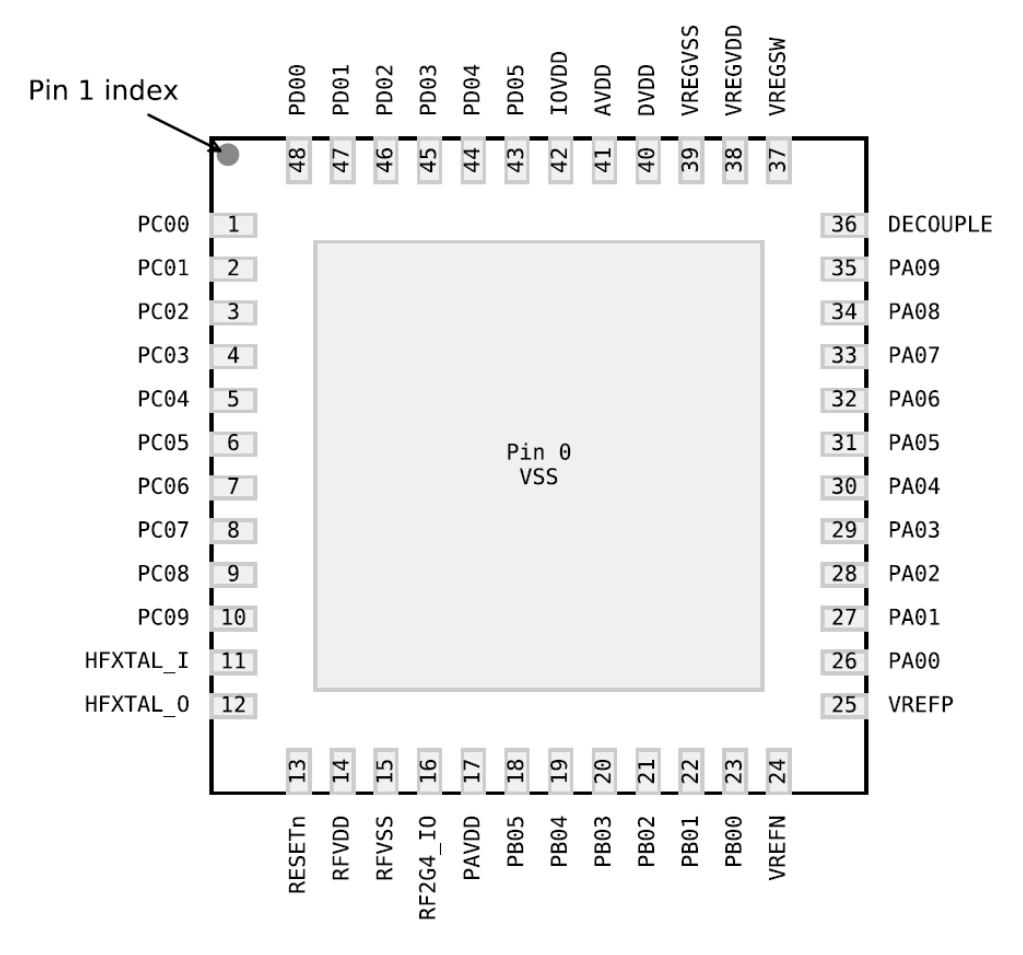
\includegraphics[keepaspectratio]{contents/core/img/chapter4-efr32-pinout.png}}

}

\caption{Figure 4.1: Pinout of QFN-48 packaged EFR32MG24 microcontroller
(EFR32MG24 Datasheet page 107)}

\end{figure}%%
\begin{figure}[H]

{\centering \pandocbounded{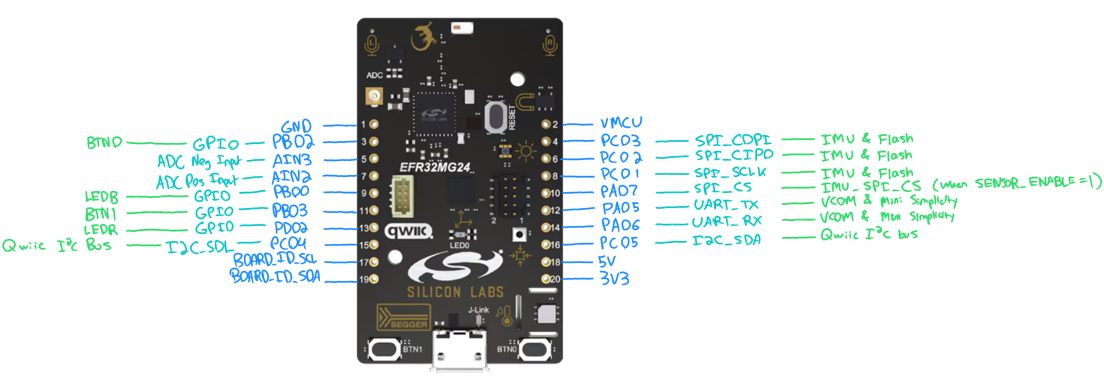
\includegraphics[keepaspectratio]{contents/core/img/chapter4-devkit-pinout.png}}

}

\caption{Figure 4.2: EFR32XG24 Dev Kit Expansion Header Pinout (UG524
page 19)}

\end{figure}%%
\begin{figure}[H]

{\centering \pandocbounded{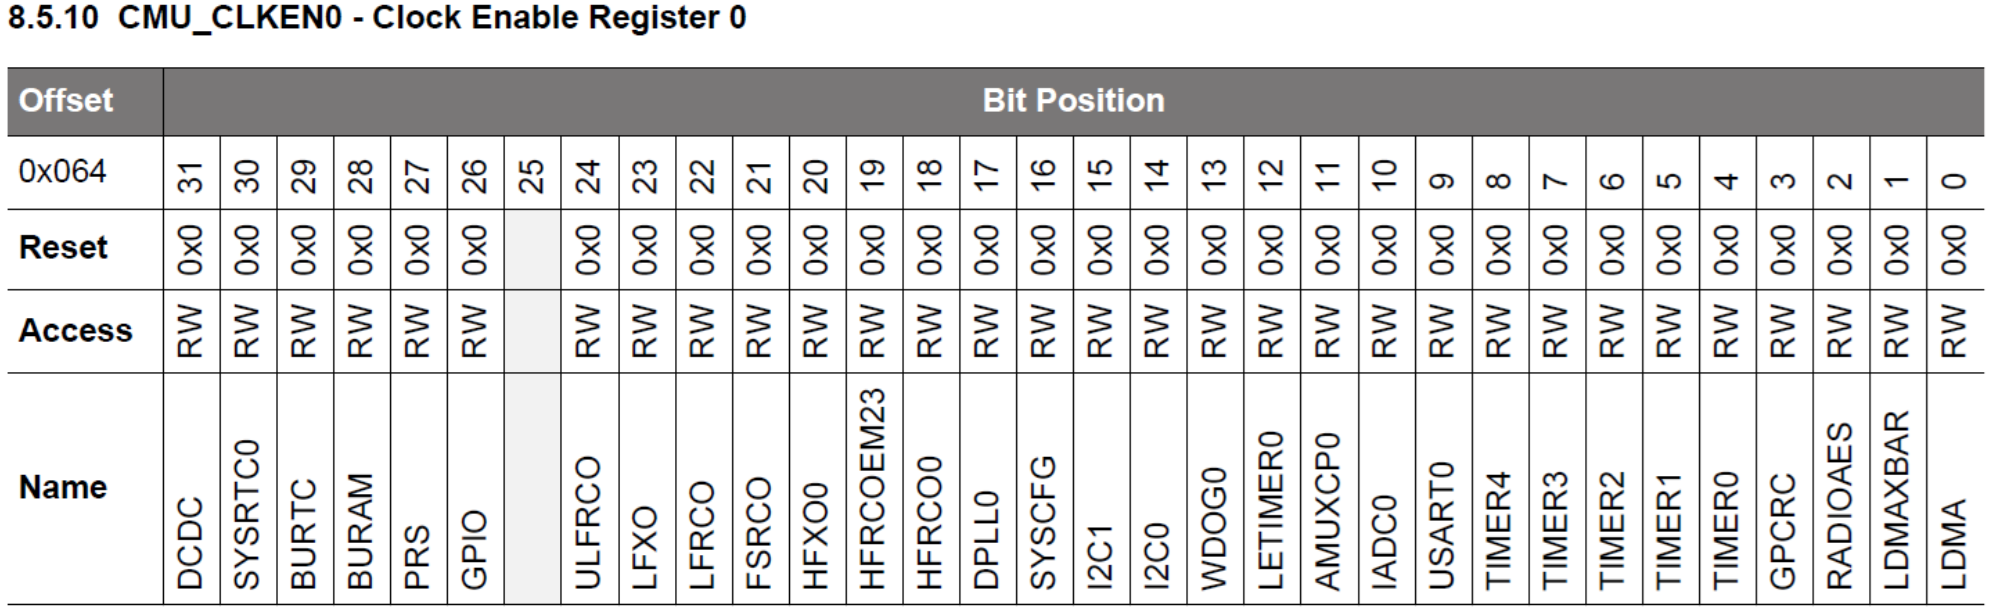
\includegraphics[keepaspectratio]{contents/core/img/chapter4-cmu-clken0.png}}

}

\caption{Figure 4.3: Peripherals available to enable in the CMU\_CLKEN0
register (Reference manual page 173)}

\end{figure}%%
\begin{figure}[H]

{\centering \pandocbounded{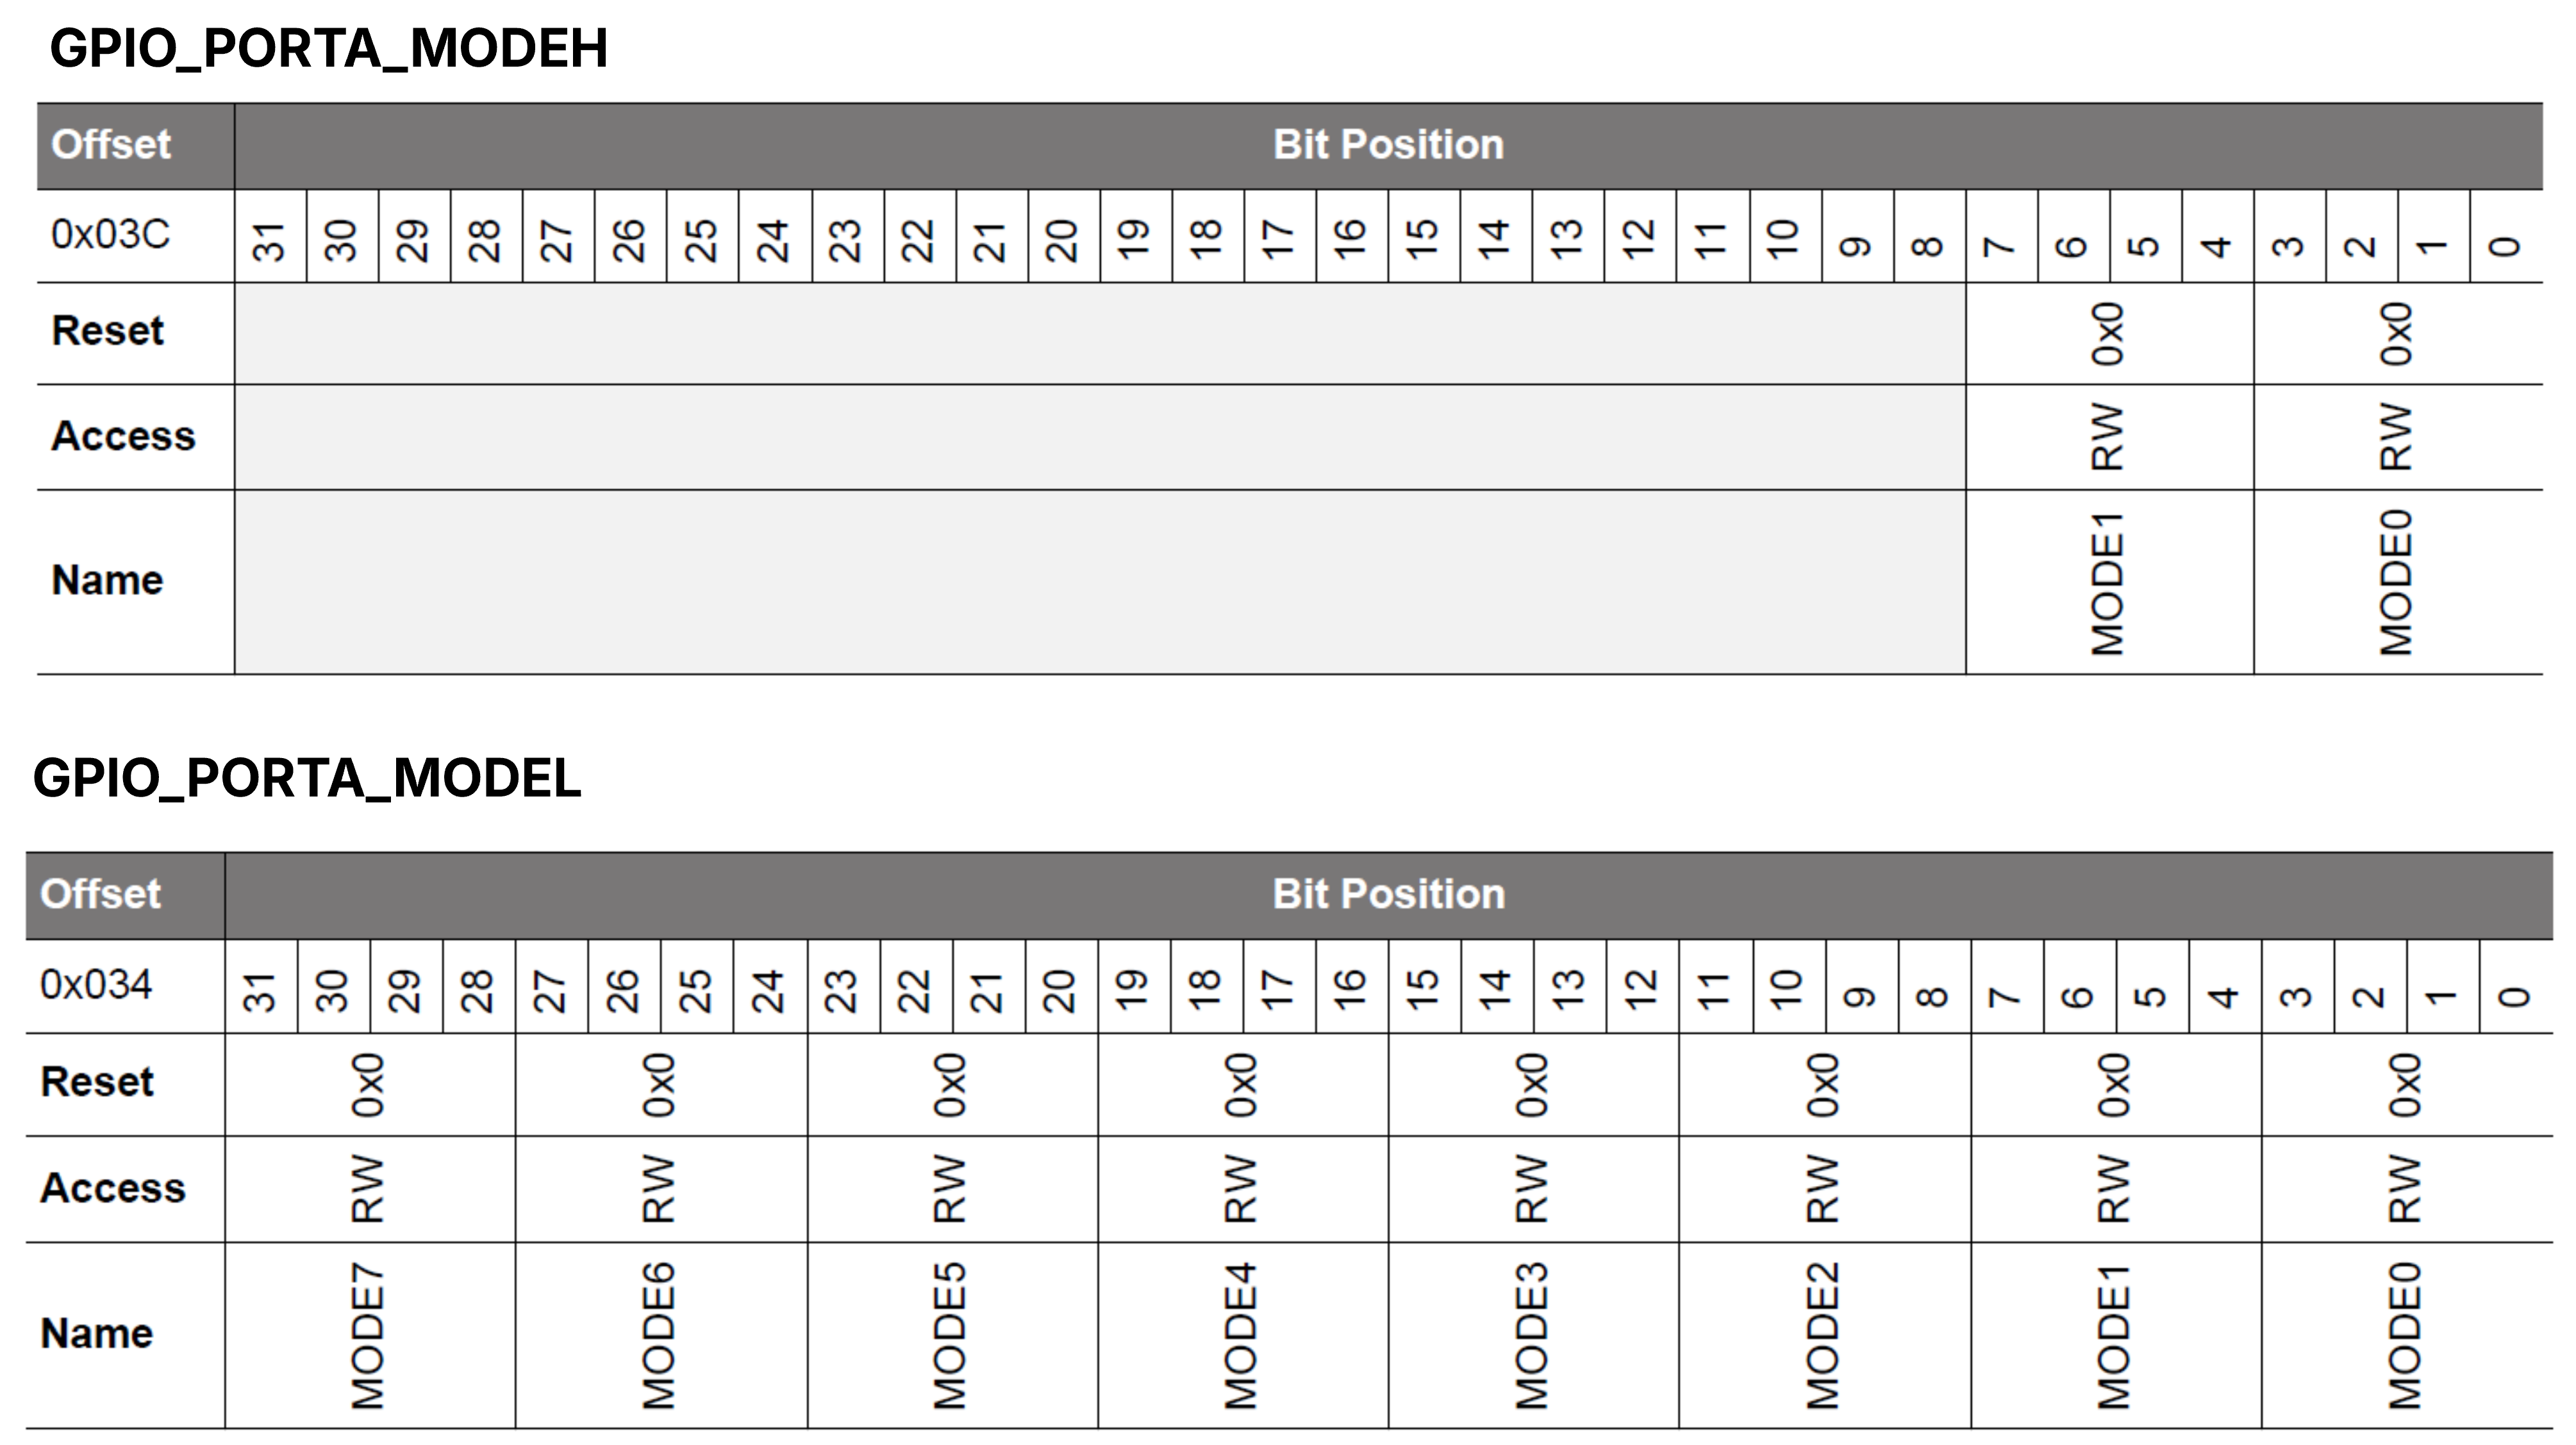
\includegraphics[keepaspectratio]{contents/core/img/chapter4-model-modeh.png}}

}

\caption{Figure 4.4: The MODEL and MODEH registers for EFR32MG24 GPIO
Port A (Reference manual page 851)}

\end{figure}%

\subsection{GPIO Configuration}\label{gpio-configuration}

Each GPIO pin can serve multiple functions controlled by the MODEL and
MODEH registers:

\begin{itemize}
\item
  \textbf{MODEL:} Configures pins 0-7 of the port.
\item
  \textbf{MODEH:} Configures pins 8-15 of the port.
\end{itemize}

Each pin mode is represented by 4 bits, supporting modes such as:

\begin{itemize}
\item
  0: Disabled
\item
  1: Input
\item
  2: Input pull-up/down
\item
  4: Push-pull (Output)
\end{itemize}

In pull-up/pull-down mode, the value of the \texttt{DOUT} register
(covered later) determines the pull direction, with a \texttt{1} being
pull-up and \texttt{0} being pull-down.

To set a pin mode programmatically:

\begin{Shaded}
\begin{Highlighting}[]
\NormalTok{GPIO}\OperatorTok{{-}\textgreater{}}\NormalTok{P}\OperatorTok{[}\NormalTok{gpioPortX}\OperatorTok{].}\NormalTok{MODEL }\OperatorTok{|=}\NormalTok{ mode }\OperatorTok{\textless{}\textless{}} \OperatorTok{(}\DecValTok{4} \OperatorTok{*}\NormalTok{ n}\OperatorTok{);}
\end{Highlighting}
\end{Shaded}

For pin numbers 8-15:

\begin{Shaded}
\begin{Highlighting}[]
\NormalTok{GPIO}\OperatorTok{{-}\textgreater{}}\NormalTok{P}\OperatorTok{[}\NormalTok{gpioPortX}\OperatorTok{].}\NormalTok{MODEH }\OperatorTok{|=}\NormalTok{ mode }\OperatorTok{\textless{}\textless{}} \OperatorTok{(}\DecValTok{4} \OperatorTok{*} \OperatorTok{(}\NormalTok{n }\OperatorTok{{-}} \DecValTok{8}\OperatorTok{));}
\end{Highlighting}
\end{Shaded}

A total of 16 pin modes are available for each GPIO pin. While many of
these modes are not used in basic applications, Figure
\hyperref[fig:moden]{4.5} displays all of the available options.

\begin{figure}

{\centering \pandocbounded{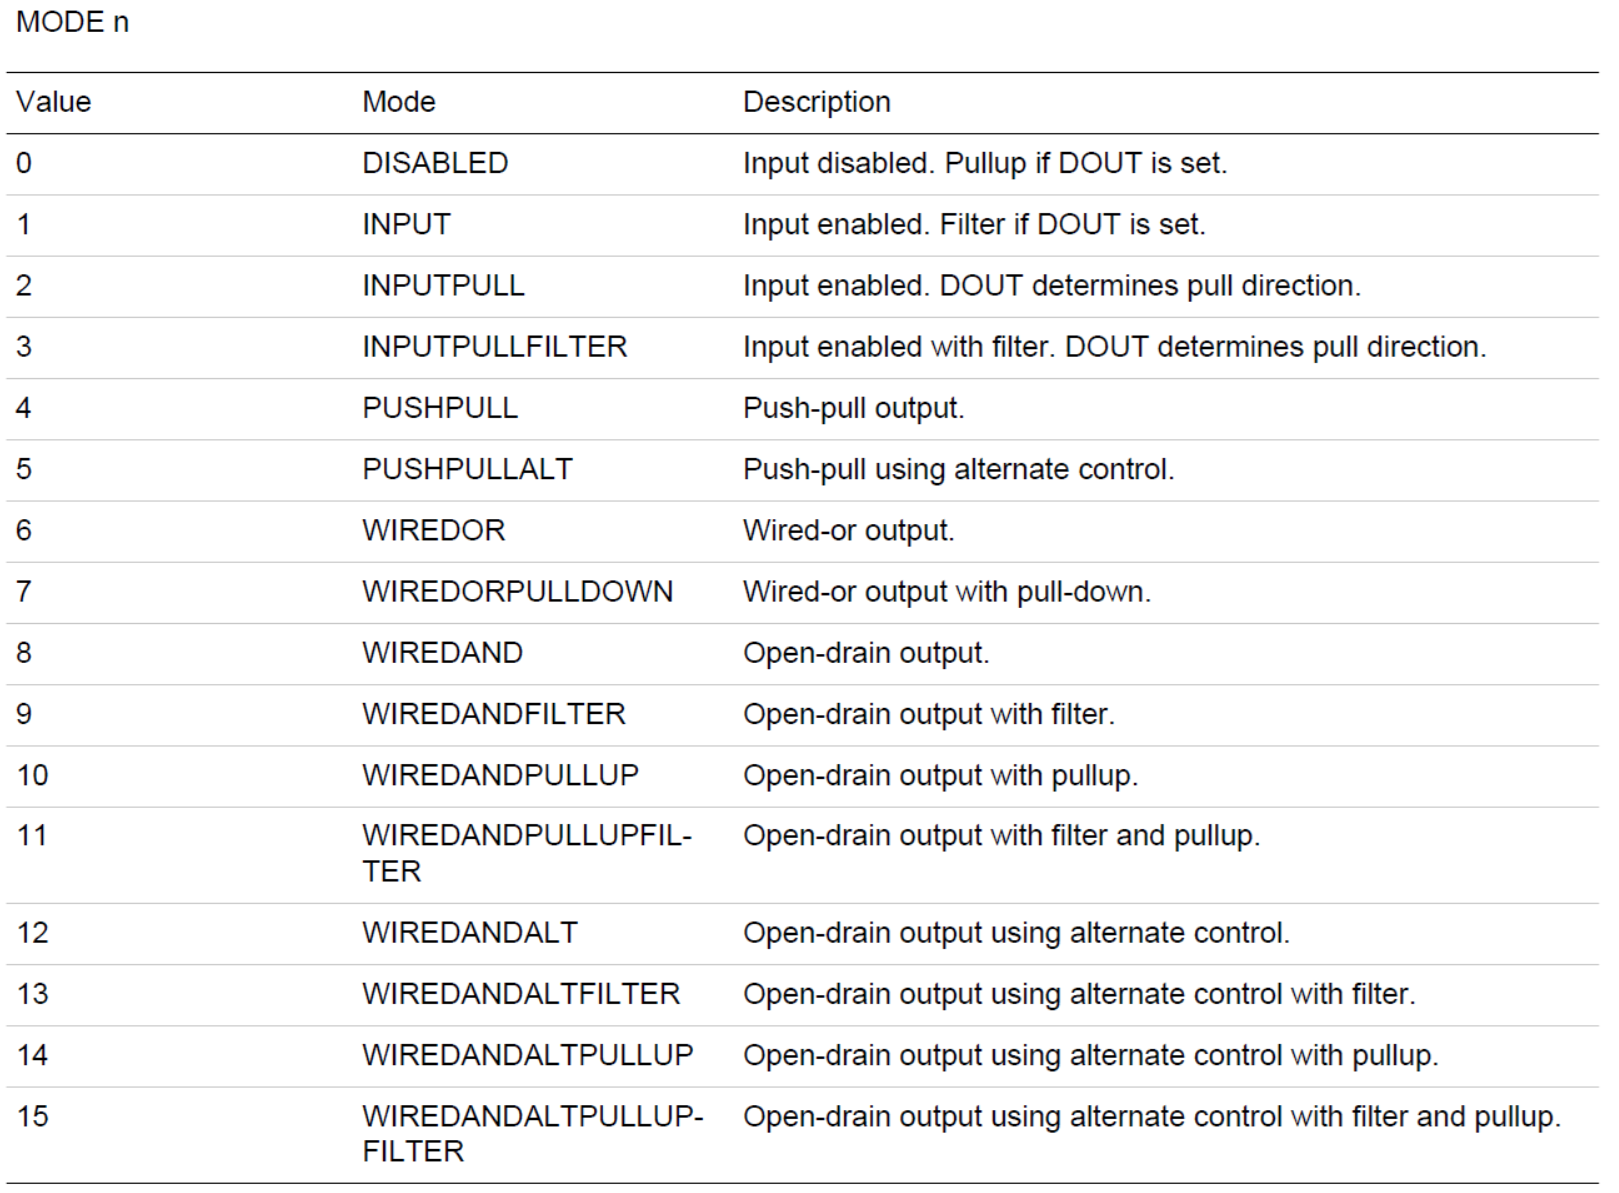
\includegraphics[keepaspectratio]{contents/core/img/chapter4-mode-n.png}}

}

\caption{Figure 4.5: Mode register value options for each GPIO pin
(Reference manual page 851)}

\end{figure}%

\subsection{GPIO Output Control}\label{gpio-output-control}

GPIO output can be managed using the following registers:

\begin{itemize}
\item
  \textbf{DOUT:} Directly outputs data to pins.
\item
  \textbf{SET:} Atomically sets specified bits.
\item
  \textbf{CLR:} Atomically clears specified bits.
\item
  \textbf{TGL:} Atomically toggles specified bits.
\end{itemize}

Example of setting and clearing pins:

\begin{Shaded}
\begin{Highlighting}[]
\NormalTok{GPIO}\OperatorTok{{-}\textgreater{}}\NormalTok{P}\OperatorTok{[}\NormalTok{gpioPortD}\OperatorTok{].}\NormalTok{DOUT }\OperatorTok{|=} \DecValTok{1} \OperatorTok{\textless{}\textless{}} \DecValTok{2}\OperatorTok{;} \CommentTok{// Set pin 2 of Port D}
\NormalTok{GPIO}\OperatorTok{{-}\textgreater{}}\NormalTok{P}\OperatorTok{[}\NormalTok{gpioPortD}\OperatorTok{].}\NormalTok{DOUT }\OperatorTok{\&=} \OperatorTok{\textasciitilde{}(}\DecValTok{1} \OperatorTok{\textless{}\textless{}} \DecValTok{2}\OperatorTok{);} \CommentTok{// Clear pin 2 of Port D}
\end{Highlighting}
\end{Shaded}

\subsection{GPIO Input Control}\label{gpio-input-control}

GPIO pins configured as inputs can be read using the DIN register:

\begin{Shaded}
\begin{Highlighting}[]
\DataTypeTok{uint8\_t}\NormalTok{ pinState }\OperatorTok{=} \OperatorTok{(}\NormalTok{GPIO}\OperatorTok{{-}\textgreater{}}\NormalTok{P}\OperatorTok{[}\NormalTok{gpioPortX}\OperatorTok{].}\NormalTok{DIN }\OperatorTok{\textgreater{}\textgreater{}}\NormalTok{ n}\OperatorTok{)} \OperatorTok{\&} \DecValTok{1}\OperatorTok{;}
\end{Highlighting}
\end{Shaded}

This reads the state of pin \texttt{n} and returns either 0 or 1.

\subsection{Using emlib for GPIO}\label{using-emlib-for-gpio}

EFR32 provides the \textbf{emlib} hardware abstraction layer (HAL) for
GPIO configuration:

\begin{itemize}
\item
  GPIO\_PinModeSet(port, pin, mode)
\item
  GPIO\_PinOutSet(port, pin)
\item
  GPIO\_PinOutClear(port, pin)
\item
  GPIO\_PinOutToggle(port, pin)
\item
  GPIO\_PinInGet(port, pin)
\end{itemize}

Example of setting a pin as output using emlib:

\begin{Shaded}
\begin{Highlighting}[]
\NormalTok{GPIO\_PinModeSet}\OperatorTok{(}\NormalTok{gpioPortD}\OperatorTok{,} \DecValTok{2}\OperatorTok{,}\NormalTok{ gpioModePushPull}\OperatorTok{);} \CommentTok{// Set the Push Pull Mode of Pin 2 of Port D}
\NormalTok{GPIO\_PinOutSet}\OperatorTok{(}\NormalTok{gpioPortD}\OperatorTok{,} \DecValTok{2}\OperatorTok{);} \CommentTok{// Set pin 2 of Port D}
\end{Highlighting}
\end{Shaded}

\subsection{Practical Example: Blinking an
LED}\label{practical-example-blinking-an-led}

A simple example of GPIO programming is blinking an LED connected to a
GPIO pin:

\begin{Shaded}
\begin{Highlighting}[]
\NormalTok{GPIO\_PinModeSet}\OperatorTok{(}\NormalTok{gpioPortD}\OperatorTok{,} \DecValTok{2}\OperatorTok{,}\NormalTok{ gpioModePushPull}\OperatorTok{);}
\ControlFlowTok{while} \OperatorTok{(}\DecValTok{1}\OperatorTok{)} \OperatorTok{\{}
\NormalTok{    GPIO\_PinOutToggle}\OperatorTok{(}\NormalTok{gpioPortD}\OperatorTok{,} \DecValTok{2}\OperatorTok{);}
\NormalTok{    delay}\OperatorTok{(}\DecValTok{1000}\OperatorTok{);}
\OperatorTok{\}}
\end{Highlighting}
\end{Shaded}

This toggles the LED state every second.

\chapter{\texorpdfstring{\textbf{Applications of EFR32
I/O}}{Applications of EFR32 I/O}}\label{applications-of-efr32-io}

Now that the basics of EFR32XG24 microcontroller input/output (I/O) are
understood, the next step is learning how to add additional
functionality to embedded systems using more complex hardware. This
chapter will prepare readers to interact with more complex off-chip
hardware using the microcontroller's GPIO pins, and is an important step
towards building user-friendly and effective embedded systems.

\section{7-Segment Displays}\label{segment-displays}

7-segment displays are commonly found in user-facing embedded systems,
such as clock radios, household appliances, vehicles, and industrial
equipment. While LED status indicators are often used for simple
devices, they cannot communicate detailed information such as sensor
readings or error codes. Gaining traction in the 1970s with the advent
of LED technology, 7-segment displays bridge the gap between basic
indicator lights and more complex graphic screens, commonly offering one
or multiple digits composed of seven LED digit segments plus a decimal
point or colon.

\subsection{Segments}\label{segments}

7-segment displays are composed of a group of LED segments arranged in
an ``8'' pattern, allowing every digit from 0-9 plus a limited selection
of letters to be readable.

These segments are commonly labeled A-G in a clockwise manner, with A
being the top segment and G being the middle segment. Depending on the
display, the segments may be wired in a common anode (LED positive
terminal) or common cathode (LED negative terminal) configuration.
Depending on the configuration, a slightly different circuit with
inverted code logic may be necessary.

Additionally, as each segment is a simple LED, current-limiting
resistors are a necessary inclusion in the circuit. In some cases, it
may be acceptable to place a single resistor between in series with the
common pin, especially if the resistor is of a high value to
significantly limit the segment's brightness. However, in most cases, it
is ideal to adhere to the best practice of placing a current-limiting
resistor in series with each \emph{segment} so that manufacturing
discrepancies between segments do not allow any individual segment to
endanger itself with a high current.

\subsection{Wiring}\label{wiring}

A 7-segment display will allocate a significant number of pins on a
microcontroller, often using up nearly an entire GPIO port. If the
decimal point is not used, one pin may be saved, but in many cases, it
is beneficial to use a BCD to 7-segment decoder IC, such as the 74LS147,
or even an 8-bit serial-in, parallel-out shift register such as the
74HC595 for greater GPIO pin efficiency. However, for the purposes of
this guide, the 7-segment display will be directly connected to the
microcontroller, using 8 GPIO pins.

In an ideal design, such as when building a PCB carrier board for the
EFR32MG24 chip, a bank of pins such as PC00-PC07 may be used, allowing
the GPIO port C MODEL register to be written in its entirety and full
bytes written to the pin set and clear ports.

However, the EFR32XG24 Dev Kit board does not break out a single port in
its entirety, therefore requiring the display to share pins between Port
A and Port C. Segments A-E will use PC01-PC05, while F, G, and the
decimal point (DP) will be connected to PA05-PA07, as displayed in
Figure \hyperref[fig:7-segment-wiring]{5.1}. This requires in code an
array of GPIO ports and pins to look up the right one for a given
segment:

\begin{Shaded}
\begin{Highlighting}[]
\CommentTok{// use gpioPortC (2) pins 1{-}5 for A{-}E, and gpioPortA (0) pins 5{-}7 for F, G, and DP}
\CommentTok{//                               A  B  C  D  E  F  G  .}
\DataTypeTok{const} \DataTypeTok{uint8\_t}\NormalTok{ segment\_ports}\OperatorTok{[]} \OperatorTok{=} \OperatorTok{\{}\DecValTok{2}\OperatorTok{,} \DecValTok{2}\OperatorTok{,} \DecValTok{2}\OperatorTok{,} \DecValTok{2}\OperatorTok{,} \DecValTok{2}\OperatorTok{,} \DecValTok{0}\OperatorTok{,} \DecValTok{0}\OperatorTok{,} \DecValTok{0}\OperatorTok{\};}
\DataTypeTok{const} \DataTypeTok{uint8\_t}\NormalTok{ segment\_pins}\OperatorTok{[]} \OperatorTok{=}  \OperatorTok{\{}\DecValTok{1}\OperatorTok{,} \DecValTok{2}\OperatorTok{,} \DecValTok{3}\OperatorTok{,} \DecValTok{4}\OperatorTok{,} \DecValTok{5}\OperatorTok{,} \DecValTok{5}\OperatorTok{,} \DecValTok{6}\OperatorTok{,} \DecValTok{7}\OperatorTok{\};}
\end{Highlighting}
\end{Shaded}

\begin{figure}

{\centering \pandocbounded{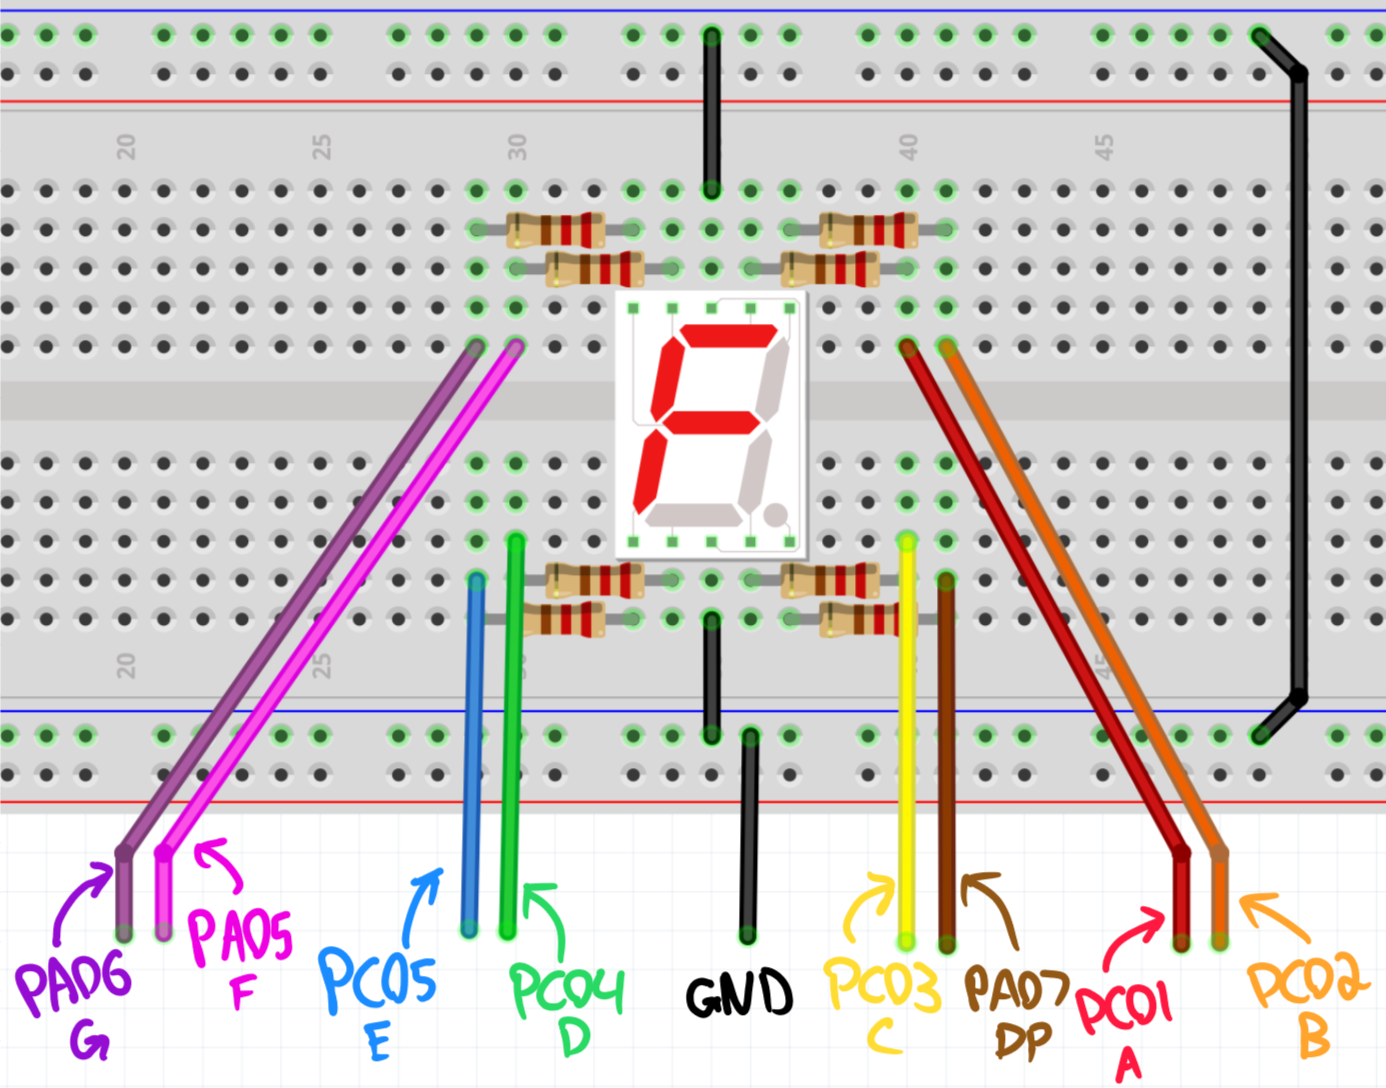
\includegraphics[keepaspectratio]{contents/core/img/chapter5-segment-wiring.png}}

}

\caption{Figure 5.1: Wiring diagram for a single common cathode
7-segment display}

\end{figure}%

\subsection{Digit display logic}\label{digit-display-logic}

With these arrays created, the pattern of segments to enable for any
character can now be defined. As there are eight segments in total, it
makes sense to represent these patterns as bits in a byte, allowing for
straightforward storage and lookup. To construct this byte, one may
represent segment A as bit 0, B as bit 1, and so on until DP is bit 7.
This results in Table \hyperref[table:7segmentlookuptable]{5.1},
displaying the construction of hexadecimal codes for digits 0-9.

\phantomsection\label{table:7segmentlookuptable}
\begin{longtable}[]{@{}
  >{\centering\arraybackslash}p{(\linewidth - 18\tabcolsep) * \real{0.1000}}
  >{\centering\arraybackslash}p{(\linewidth - 18\tabcolsep) * \real{0.1000}}
  >{\centering\arraybackslash}p{(\linewidth - 18\tabcolsep) * \real{0.1000}}
  >{\centering\arraybackslash}p{(\linewidth - 18\tabcolsep) * \real{0.1000}}
  >{\centering\arraybackslash}p{(\linewidth - 18\tabcolsep) * \real{0.1000}}
  >{\centering\arraybackslash}p{(\linewidth - 18\tabcolsep) * \real{0.1000}}
  >{\centering\arraybackslash}p{(\linewidth - 18\tabcolsep) * \real{0.1000}}
  >{\centering\arraybackslash}p{(\linewidth - 18\tabcolsep) * \real{0.1000}}
  >{\centering\arraybackslash}p{(\linewidth - 18\tabcolsep) * \real{0.1000}}
  >{\centering\arraybackslash}p{(\linewidth - 18\tabcolsep) * \real{0.1000}}@{}}
\toprule\noalign{}
\endfirsthead
\endhead
\bottomrule\noalign{}
\tabularnewline
\caption{Lookup table for 7-segment display digit codes}\tabularnewline
\endlastfoot
\textbf{Digit} & \textbf{bit 7} & \textbf{bit 6} & \textbf{bit 5} &
\textbf{bit 4} & \textbf{bit 3} & \textbf{bit 2} & \textbf{bit 1} &
\textbf{bit 0} & \textbf{Hexadecimal} \\
& \textbf{.} & \textbf{G} & \textbf{F} & \textbf{E} & \textbf{D} &
\textbf{C} & \textbf{B} & \textbf{A} & \\
\textbf{0} & 0 & 0 & 1 & 1 & 1 & 1 & 1 & 1 & \textbf{0x3F} \\
\textbf{1} & 0 & 0 & 0 & 0 & 0 & 1 & 1 & 0 & \textbf{0x06} \\
\textbf{2} & 0 & 1 & 0 & 1 & 1 & 0 & 1 & 1 & \textbf{0x5B} \\
\textbf{3} & 0 & 1 & 0 & 0 & 1 & 1 & 1 & 1 & \textbf{0x4F} \\
\textbf{4} & 0 & 1 & 1 & 0 & 0 & 1 & 1 & 0 & \textbf{0x66} \\
\textbf{5} & 0 & 1 & 1 & 0 & 1 & 1 & 0 & 1 & \textbf{0x6D} \\
\textbf{6} & 0 & 1 & 1 & 1 & 1 & 1 & 0 & 1 & \textbf{0x7D} \\
\textbf{7} & 0 & 0 & 0 & 0 & 0 & 1 & 1 & 1 & \textbf{0x07} \\
\textbf{8} & 0 & 1 & 1 & 1 & 1 & 1 & 1 & 1 & \textbf{0x7F} \\
\textbf{9} & 0 & 1 & 1 & 0 & 1 & 1 & 1 & 1 & \textbf{0x6F} \\
\end{longtable}

These hexadecimal codes for each digit can then be inserted into another
array, with the array index mapping a desired digit to its segment code.
In a later exercise, you will be required to expand this array to
support hexadecimal digits as well.

\subsection{Display driver code}\label{display-driver-code}

Now that this look-up array for digits is implemented, driving the
7-segment display is trivial. Each GPIO pin in use must be set up as an
output. Each pin may then be looped through, and set or cleared
depending on if its corresponding bit in the hexadecimal code is set.
This can be achieved by shifting the hexadecimal code right by the loop
iterator variable, then evaluating based on the bitwise AND of the
shifted code and 1.

\begin{Shaded}
\begin{Highlighting}[]
\ControlFlowTok{for} \OperatorTok{(}\DataTypeTok{int}\NormalTok{ i }\OperatorTok{=} \DecValTok{0}\OperatorTok{;}\NormalTok{ i }\OperatorTok{\textless{}} \DecValTok{8}\OperatorTok{;}\NormalTok{ i}\OperatorTok{++)} \CommentTok{// loop through all segments}
\OperatorTok{\{} 
    \ControlFlowTok{if} \OperatorTok{((}\NormalTok{segments}\OperatorTok{[}\NormalTok{arbitrary\_digit}\OperatorTok{]} \OperatorTok{\textgreater{}\textgreater{}}\NormalTok{ i}\OperatorTok{)} \OperatorTok{\&} \DecValTok{1}\OperatorTok{)} \CommentTok{// look up hex code, shift right, AND}
    \OperatorTok{\{}
\NormalTok{        GPIO}\OperatorTok{{-}\textgreater{}}\NormalTok{P\_SET}\OperatorTok{[}\NormalTok{segment\_ports}\OperatorTok{[}\NormalTok{i}\OperatorTok{]].}\NormalTok{DOUT }\OperatorTok{=} \DecValTok{1} \OperatorTok{\textless{}\textless{}}\NormalTok{ segment\_pins}\OperatorTok{[}\NormalTok{i}\OperatorTok{];} \CommentTok{// turn on segment}
    \OperatorTok{\}}
    \ControlFlowTok{else}
    \OperatorTok{\{}
\NormalTok{        GPIO}\OperatorTok{{-}\textgreater{}}\NormalTok{P\_CLR}\OperatorTok{[}\NormalTok{segment\_ports}\OperatorTok{[}\NormalTok{i}\OperatorTok{]].}\NormalTok{DOUT }\OperatorTok{=} \DecValTok{1} \OperatorTok{\textless{}\textless{}}\NormalTok{ segment\_pins}\OperatorTok{[}\NormalTok{i}\OperatorTok{];} \CommentTok{// turn off segment}
    \OperatorTok{\}}
\OperatorTok{\}}
\end{Highlighting}
\end{Shaded}

In this example, we use the \texttt{segments} array to loop up the hex
code for a given \texttt{arbitrary\_digit}, which could be an integer
literal or a variable. The looked up code is shifted right based on the
index of the current digit to be illuminated or turned off. With the bit
of interest now moved to bit 0, it is compared with 1 to determine the
appropriate state for the segment.

\subsection{Multiple digits}\label{multiple-digits}

In many applications, multiple 7-segment digits are necessary to display
a larger number or other more detailed information. Even displaying time
in a 12- or 24-hour format requires four digits. Therefore, it is often
beneficial to combine multiple 7-segment displays into a single module,
and these are commonly available in 2, 4, 6, or 8 digit configurations.
However, using 8 GPIO pins per segment can quickly waste all available
microcontroller pins. Instead, all digits in a module \emph{multiplex},
or share, segment pins, which means that all segments, if illuminated at
the same time, would show the same character. To facilitate this
multiplexing, each digit has its own separate common cathode or common
anode pin, which can be connected or disconnected to power. Each digit
may then be lit one after another, with only one on at a given time, and
this process is constantly repeated to create the effect that all digits
are constantly on.

This does necessitate the use of an NPN transistor for each digit to
switch the common pin load of the digit on and off, as the
microcontroller cannot sink this significant current into a single GPIO.
An example circuit is included in Figure
\hyperref[fig:multi-digit-7-segment-schematic]{5.2}, demonstrating the
connections of a two-digit module with a common cathode configuration to
an MCU.

\subsection{Multiple digits logic}\label{multiple-digits-logic}

The same code may be used for driving multiple digits as a single digit;
after all, the only difference is that the lit digit must be changed
repeatedly. It is therefore ideal to move the single digit driver code
to its own function so that it may be reused. The infinite loop must be
adjusted to drive each digit's transistor base pin high, then display a
given digit, and finally switch the transistor back off before repeating
the process for the next digit. This must be done quickly to avoid
flicker at a frequency that is visible to the human eye, but not so
quickly that the LEDs in each segment do not have time to reach their
full brightness. Therefore, a few milliseconds of delay may be necessary
while each digit is on before quickly switching to the next digit.

\begin{figure}

{\centering \pandocbounded{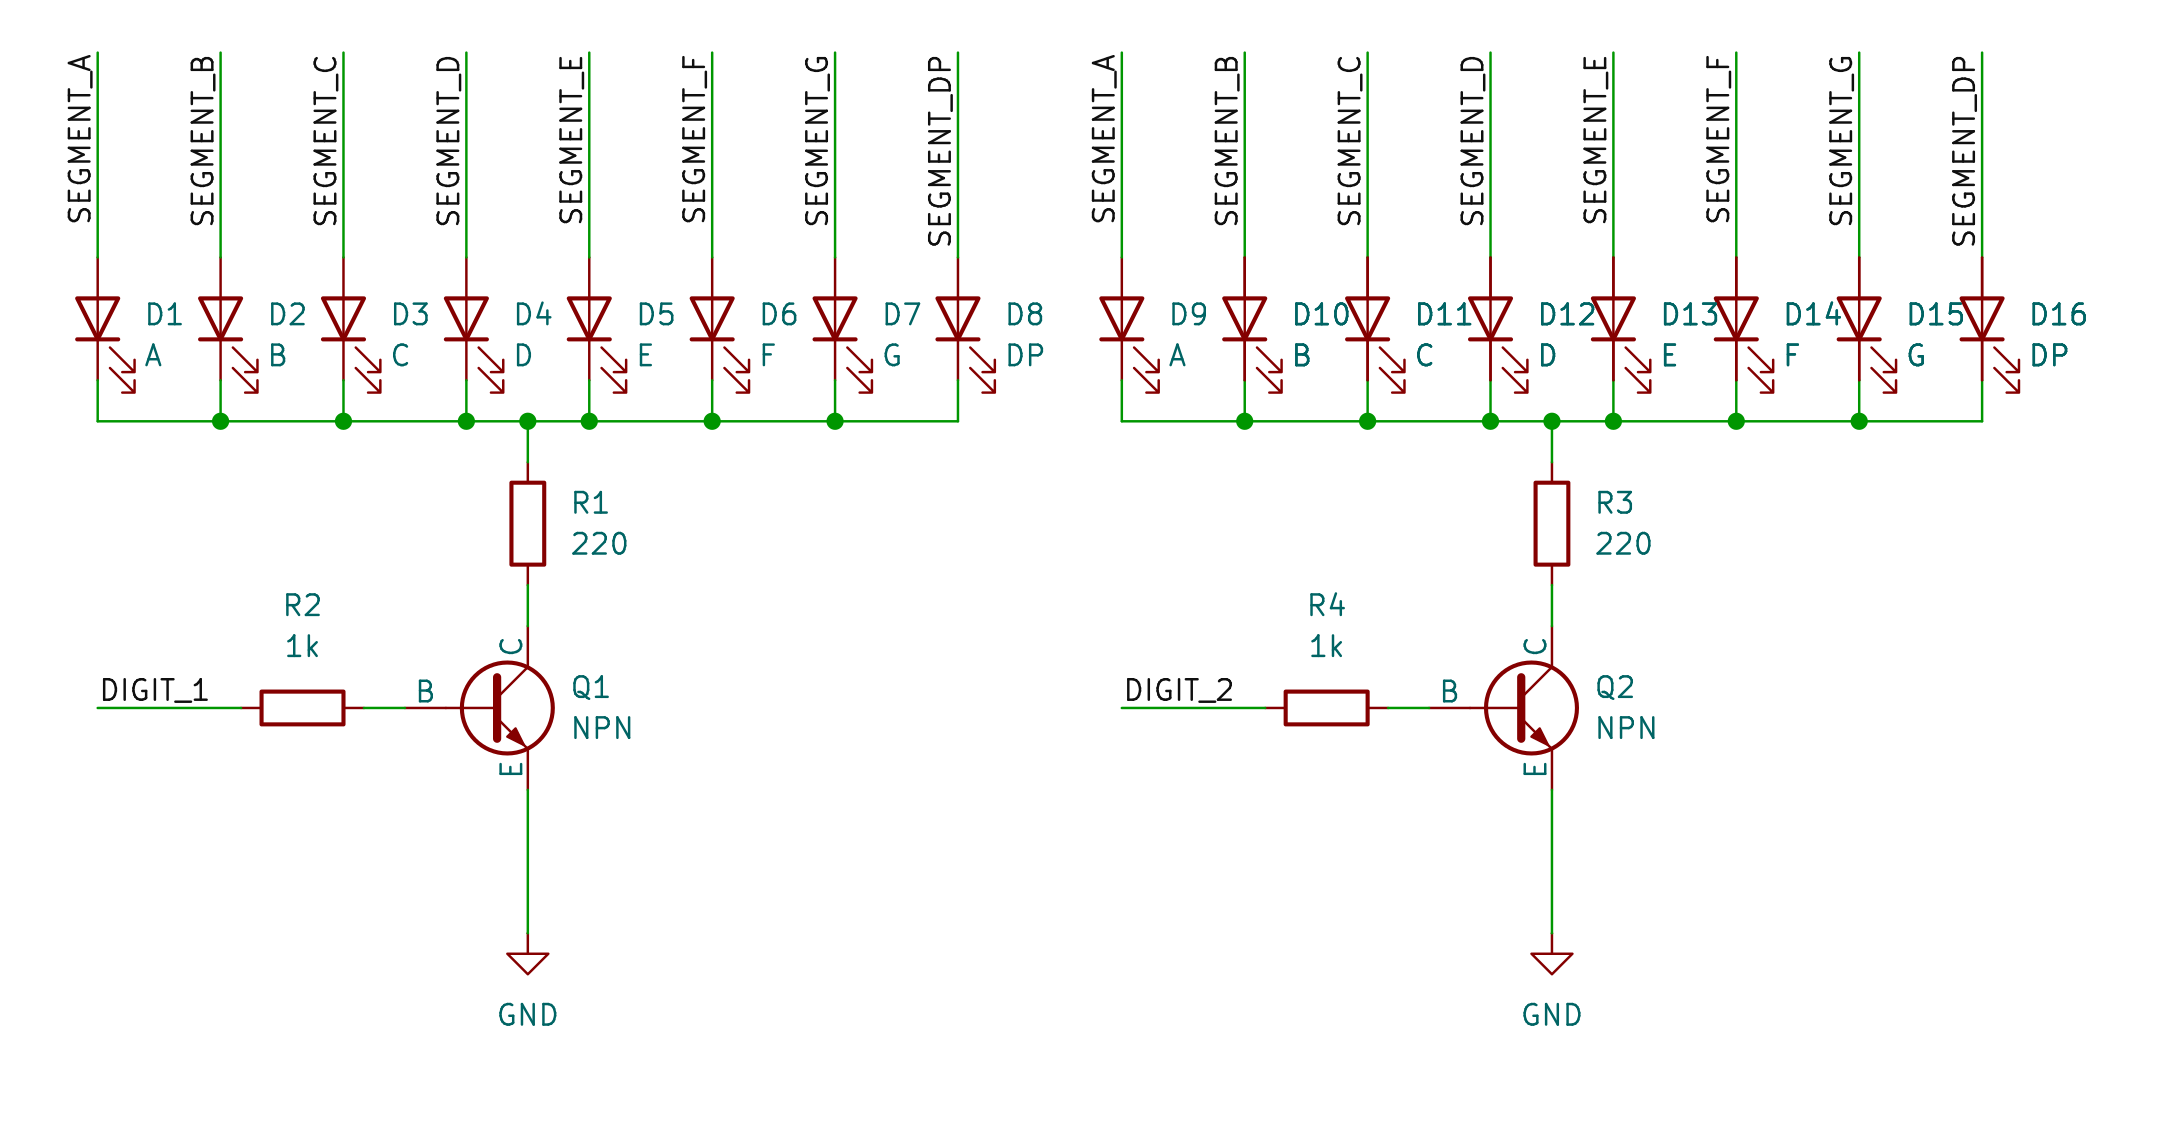
\includegraphics[keepaspectratio]{contents/core/img/chapter5-segment-multi-schematic.png}}

}

\caption{Figure 5.2: Two common-cathode 7-segment display digits
switches by transistors}

\end{figure}%

\subsection{Exercise: Displaying hexadecimal
numbers}\label{exercise-displaying-hexadecimal-numbers}

Complete Table \hyperref[table:7segmentlookuptable]{5.1} with the
additional hexadecimal digits A-F, and expand the array. Then, try
displaying 8-bit numbers in hexadecimal format with a two-digit
7-segment display module.

\section{Parallel LCD displays}\label{parallel-lcd-displays}

When more letters or symbols must be displayed to a user than is
practical with a simple 7-segment display, or a graphical user interface
is it is common to use a screen. Early computers generated signals to
drive CRT screens, with a limited number of display lines and colors.
Now, while full-color, high resolution monitors and other displays are
widespread, it is still common to find smaller, often monochrome screens
used in embedded systems due to their simplicity and minimal power
consumption. In this section, we will learn about interfacing with a
liquid crystal display (LCD) screen that can display two lines of 5x8
pixel characters. These low-cost displays are commonly found on budget
3D printers, control units for machinery, or in vehicle entertainment
systems.

\subsection{16x2 Character LCD}\label{x2-character-lcd}

An inexpensive character-based LCD module often contains 2-4 rows of
8-20 characters. In this case, the common LCD1602 module with 2 rows of
16 characters will be used. At the top of the display is a row of pins
for powering and controlling the display. Table
\hyperref[table:16x2lcdpins]{5.2} displays details for each pin, but
most commonly found on these displays are power and ground for the
display, a separate anode and cathode for the backlight LED, a contrast
adjustment, and a number of data and control signals. To understand how
to interface with the LCD, we must examine the display's built in
controller.

\subsection{LCD Controller}\label{lcd-controller}

The LCD module has an on-board Hitachi HD44780U controller that
generates signals for the individual pixels of the display. The HD44780U
is based on an original 1980s design, retaining command and feature
parity while supporting modern microcontroller interfaces. It has two
host-facing I/O registers as well as internal memory, meaning that data
written to the display remains until it is next updated, reducing host
MCU processor load. A 4- and 8-bit interface allows writing to, or
reading from, both the instruction register or data register, which are
used for configuration and character output, respectively. Therefore,
these displays are known as using a parallel interface, as multiple bits
of data are transferred at the same instant. More advanced displays may
also offer additional interfaces that we will learn about later, such as
I\textsuperscript{2}C or SPI. It is important to read and understand the
datasheet for the LCD controller to learn how to interface with it. The
datasheet is linked here, but excerpts will be taken from it in this
section: \url{https://www.sparkfun.com/datasheets/LCD/HD44780.pdf}

\begin{figure}[H]

{\centering \pandocbounded{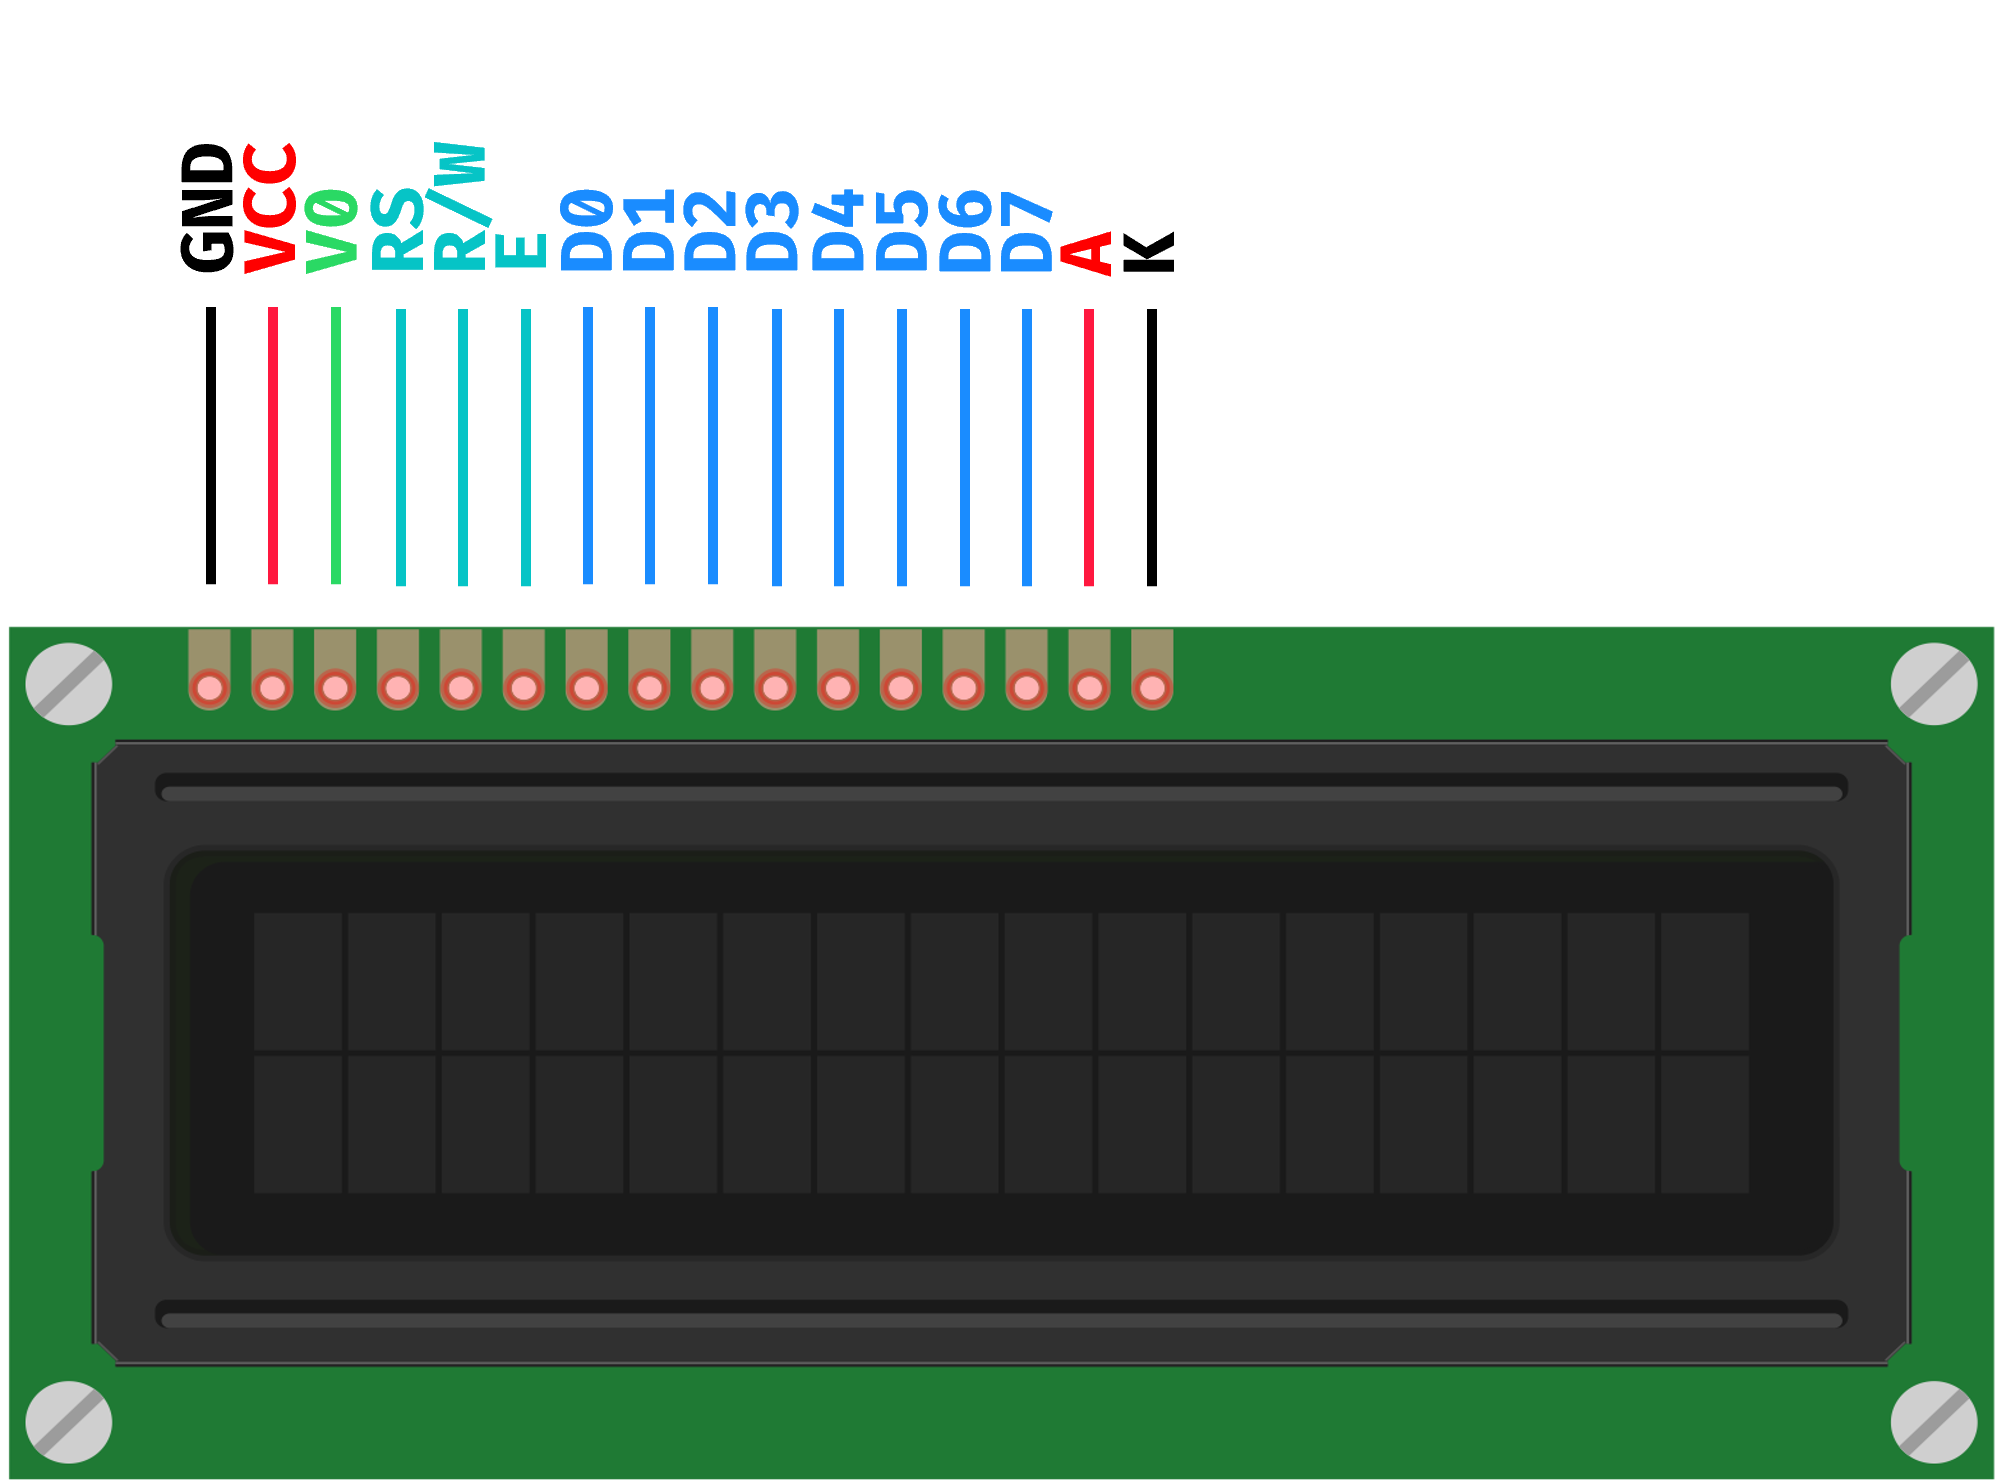
\includegraphics[keepaspectratio]{contents/core/img/chapter5-lcd-pins.png}}

}

\caption{Figure 5.3: Pinout for commonly available 16x2 LCD modules}

\end{figure}%

\phantomsection\label{table:16x2lcdpins}
\begin{longtable}[]{@{}
  >{\raggedright\arraybackslash}p{(\linewidth - 4\tabcolsep) * \real{0.1268}}
  >{\raggedright\arraybackslash}p{(\linewidth - 4\tabcolsep) * \real{0.1690}}
  >{\raggedright\arraybackslash}p{(\linewidth - 4\tabcolsep) * \real{0.7042}}@{}}
\toprule\noalign{}
\begin{minipage}[b]{\linewidth}\raggedright
\textbf{Pin}
\end{minipage} & \begin{minipage}[b]{\linewidth}\raggedright
\textbf{Symbol}
\end{minipage} & \begin{minipage}[b]{\linewidth}\raggedright
\textbf{Description}
\end{minipage} \\
\midrule\noalign{}
\endfirsthead
\toprule\noalign{}
\begin{minipage}[b]{\linewidth}\raggedright
\textbf{Pin}
\end{minipage} & \begin{minipage}[b]{\linewidth}\raggedright
\textbf{Symbol}
\end{minipage} & \begin{minipage}[b]{\linewidth}\raggedright
\textbf{Description}
\end{minipage} \\
\midrule\noalign{}
\endhead
\bottomrule\noalign{}
\tabularnewline
\caption{Table 5.2: Pin designations and descriptions for the 16x2 LCD
display}\tabularnewline
\endlastfoot
\textbf{1} & \textbf{GND} & Display ground. \\
\textbf{2} & \textbf{VCC} & Display power. Connect to 5V. \\
\textbf{3} & \textbf{V0} & Display contrast adjustment. 0-5V range. \\
\textbf{4} & \textbf{RS} & Register select. 0 for instructions, 1 for
data. \\
\textbf{5} & \textbf{R/W} & Read/write. 0 for write, 1 for read. \\
\textbf{6} & \textbf{E} & Enable. Starts data read/write operation. \\
\textbf{7} & \textbf{D0} & Data bit 0, used in 8-bit mode. \\
\textbf{8} & \textbf{D1} & Data bit 1, used in 8-bit mode. \\
\textbf{9} & \textbf{D2} & Data bit 2, used in 8-bit mode. \\
\textbf{10} & \textbf{D3} & Data bit 3, used in 8-bit mode. \\
\textbf{11} & \textbf{D4} & Data bit 4, used in 4-bit and 8-bit mode. \\
\textbf{12} & \textbf{D5} & Data bit 4, used in 4-bit and 8-bit mode. \\
\textbf{13} & \textbf{D6} & Data bit 4, used in 4-bit and 8-bit mode. \\
\textbf{14} & \textbf{D7} & Data bit 4, used in 4-bit and 8-bit mode. \\
\textbf{15} & \textbf{A} & Backlight LED anode. Connect to 5V. \\
\textbf{16} & \textbf{K} & Backlight LED cathode. Connect to GND. \\
\end{longtable}

\subsection{LCD Wiring}\label{lcd-wiring}

As referenced above, these displays support both a 4-bit and an 8-bit
data transfer mode, with the 8-bit data length allowing for faster and
simpler transmissions while the 4-bit data length increases software
complexity but requires fewer GPIO pins to be allocated.

In both cases, the display also requires three additional control
signals, \texttt{RS}, \texttt{RW}, and \texttt{E}. The \texttt{RS} line
selects between the instruction register (if set to 0), and the data
register (if set to 1) of the HD44780 controller, allowing data sent to
be interpreted as a command or a character to display. The \texttt{RW}
line configures the data pins for read or write mode, from the
perspective of the host MCU. Because the display will receive commands
and data from the MCU most of the time, the \texttt{RW} line will often
be 0, however, in some cases such as reading the address of the display
cursor or the display's busy signal, this line should be brought high.
Finally, the \texttt{E}---or enable---signal causes a data transfer to
occur. When writing to the display, the data and control lines should
first be set up, and then the enable line quickly toggled on then back
off, causing the HD44780U to accept the command or data.

In total, the 4-bit data mode will use a minimum of 7 GPIOs, and the
8-bit mode a minimum of 11 GPIOs. While they are not prohibitive, these
are significant pin allocations for a single peripheral, and care must
be taken when designing an embedded system to make good use of available
pins.

Therefore, this section will take into account the additional complexity
of the 4-bit data mode, making the 8-bit mode comparatively trivial to
implement. To begin, the LCD should be connected to the EFR32XG24 Dev
Kit as shown in the schematic in Figure \hyperref[fig:lcdschematic]{5.4}
and the wiring diagram in Figure \hyperref[fig:lcdwiring]{5.5}.

\begin{figure}[H]

{\centering \pandocbounded{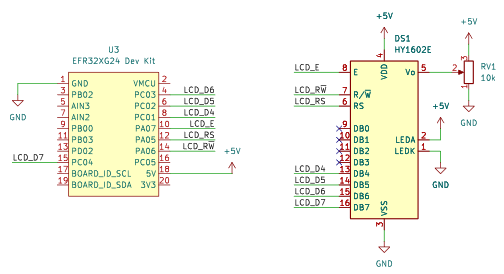
\includegraphics[keepaspectratio]{contents/core/img/chapter5-lcd-schematic.png}}

}

\caption{Figure 5.4: Schematic diagram of LCD connections to EFR32XG24
Dev Kit}

\end{figure}%%
\begin{figure}[H]

{\centering \pandocbounded{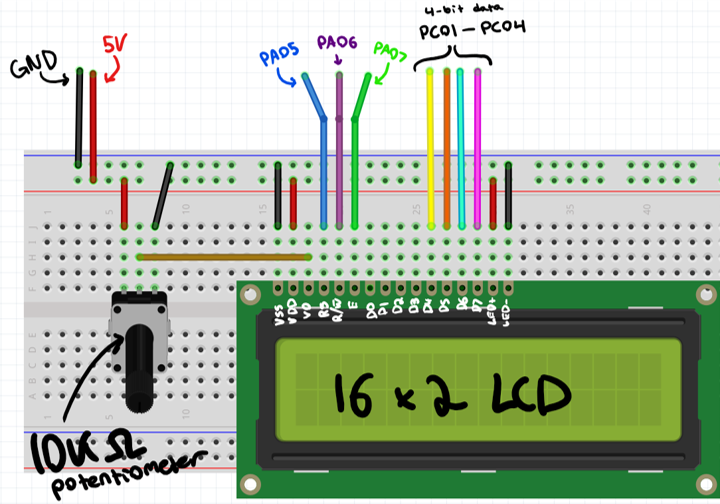
\includegraphics[keepaspectratio]{contents/core/img/chapter5-lcd-wiring.png}}

}

\caption{Figure 5.5: Wiring diagram for LCD connections to EFR32XG24 Dev
Kit}

\end{figure}%

\subsection{LCD Data Transfer}\label{lcd-data-transfer}

The LCD accepts command and data bytes on the four or eight connected
data lines, on the falling edge of a single pulse of the enable line.
The three control lines and all of the data lines must first be written
to, so that the data on them is valid at the time of the enable line
pulse. In 8-bit mode, each pulse of the enable line corresponds with a
single instruction or data. However, in 4-bit mode, two consecutive
writes or reads are necessary to transmit a full command. The command's
byte must be split into two nibbles---groups of four bits--- and then
transmitted with the most significant bits (MSBs) \texttt{7:4} first,
followed by the least significant bits (LSBs) \texttt{3:0}. At the
completion of the second data transfer, the LCD will execute the command
and, after a brief period, be ready to accept more. The following code
implements the protocol described above to send instructions or data to
the LCD. Note that this code assumes that the control and data pins have
already been configured as outputs.

\begin{Shaded}
\begin{Highlighting}[]
\DataTypeTok{void}\NormalTok{ lcd\_nibble\_write}\OperatorTok{(}\DataTypeTok{uint8\_t}\NormalTok{ data}\OperatorTok{,} \DataTypeTok{uint8\_t}\NormalTok{ register\_select}\OperatorTok{)}
\OperatorTok{\{}
\NormalTok{    lcd\_wait}\OperatorTok{();} \CommentTok{// wait until busy flag is not set (covered later in chapter)}

\NormalTok{    GPIO}\OperatorTok{{-}\textgreater{}}\NormalTok{P\_CLR}\OperatorTok{[}\NormalTok{DATA\_port}\OperatorTok{]} \OperatorTok{=}\NormalTok{ DATA\_mask}\OperatorTok{;}               \CommentTok{// clear data bits PC04{-}PC01}
\NormalTok{    GPIO}\OperatorTok{{-}\textgreater{}}\NormalTok{P\_SET}\OperatorTok{[}\NormalTok{DATA\_port}\OperatorTok{]} \OperatorTok{=} \OperatorTok{(}\NormalTok{data }\OperatorTok{\textless{}\textless{}} \DecValTok{1}\OperatorTok{)} \OperatorTok{\&}\NormalTok{ DATA\_mask}\OperatorTok{;} \CommentTok{// set data bits shifted onto the correct pins}

    \ControlFlowTok{if} \OperatorTok{(}\NormalTok{register\_select}\OperatorTok{)} \CommentTok{// data}
\NormalTok{        GPIO}\OperatorTok{{-}\textgreater{}}\NormalTok{P\_SET}\OperatorTok{[}\NormalTok{CTRL\_port}\OperatorTok{]} \OperatorTok{=} \DecValTok{1} \OperatorTok{\textless{}\textless{}}\NormalTok{ RS\_pin}\OperatorTok{;}
    \ControlFlowTok{else} \CommentTok{// command}
\NormalTok{        GPIO}\OperatorTok{{-}\textgreater{}}\NormalTok{P\_CLR}\OperatorTok{[}\NormalTok{CTRL\_port}\OperatorTok{]} \OperatorTok{=} \DecValTok{1} \OperatorTok{\textless{}\textless{}}\NormalTok{ RS\_pin}\OperatorTok{;}

\NormalTok{    GPIO}\OperatorTok{{-}\textgreater{}}\NormalTok{P\_SET}\OperatorTok{[}\NormalTok{CTRL\_port}\OperatorTok{]} \OperatorTok{=} \DecValTok{1} \OperatorTok{\textless{}\textless{}}\NormalTok{ EN\_pin}\OperatorTok{;} \CommentTok{// set enable}
\NormalTok{    sl\_sleeptimer\_delay\_millisecond}\OperatorTok{(}\DecValTok{1}\OperatorTok{);}
\NormalTok{    GPIO}\OperatorTok{{-}\textgreater{}}\NormalTok{P\_CLR}\OperatorTok{[}\NormalTok{CTRL\_port}\OperatorTok{]} \OperatorTok{=} \DecValTok{1} \OperatorTok{\textless{}\textless{}}\NormalTok{ EN\_pin}\OperatorTok{;} \CommentTok{// unset enable}
\OperatorTok{\}}
\end{Highlighting}
\end{Shaded}

The \texttt{lcd\_nibble\_write} function takes two arguments, the first
being the data (whether it be an instruction or character) to transmit,
and the second being a boolean for the register select line. First, the
function checks the LCD busy flag to determine if the LCD controller is
ready to accept new data. This function will be discussed later, and may
be implemented or replaced with a delay. The data lines are then cleared
so that any previously sent data does not interfere with the new data to
be written. As the data is expected in the lower four bits of the data
byte, it is shifted into the correct position on the port based on the
wiring diagram. Depending on the wrapper code for this function, an
additional masking of the data may be wise to avoid tampering with other
GPIO pins. The register select pin is also written to match the
\texttt{register\_select} argument, and finally the enable line toggled
to complete the transmission.

\subsection{LCD Instructions}\label{lcd-instructions}

Sending a full command or character to the LCD just requires two calls
to the already-implemented \texttt{lcd\_nibble\_write} function, one for
each nibble that must be transmitted. It may be beneficial to write a
wrapper function that does this automatically, requiring only the full
byte of data, and potentially a register select argument to complete the
entire process. This would involve shifting the data argument right four
bits, calling \texttt{lcd\_nibble\_write} to transmit these MSBs, then
masking out the upper four bits of the data argument and again calling
\texttt{lcd\_nibble\_write}.

With the understanding of sending full commands to the LCD, it can now
be properly initialized. To do so, it is necessary to consult the
HD44780U datasheet to properly form the LCD commands. An excerpt from
the datasheet is included in Figure \hyperref[fig:lcdinstructions]{5.6}.

\begin{figure}[H]

{\centering \pandocbounded{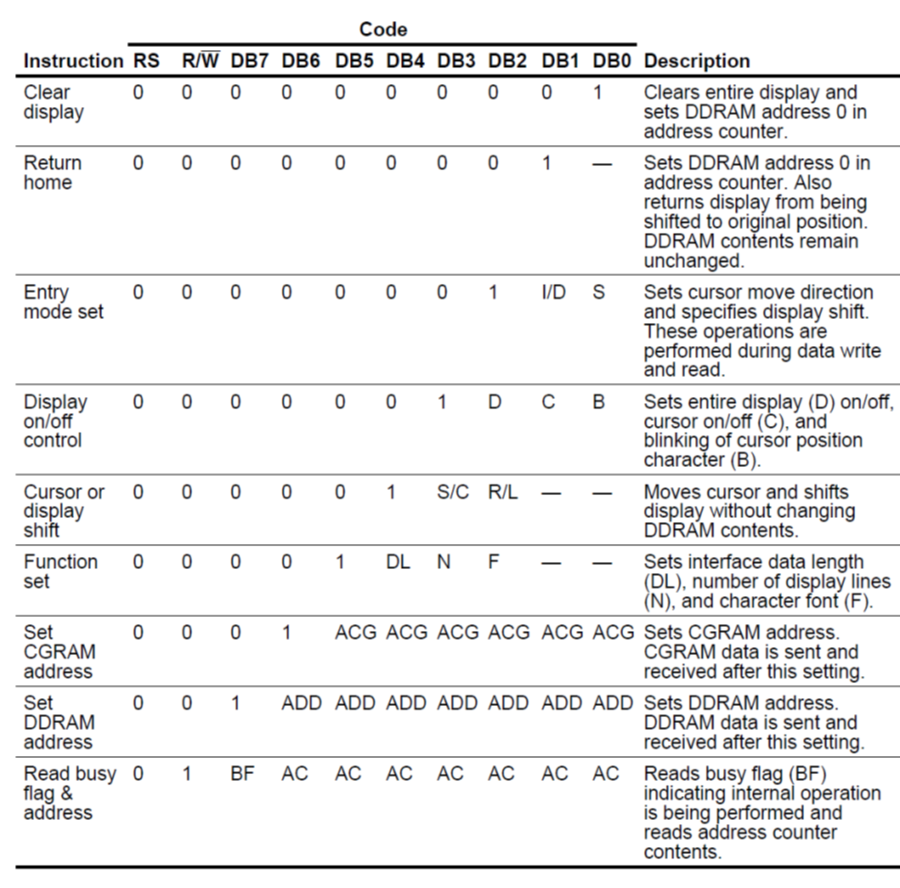
\includegraphics[keepaspectratio]{contents/core/img/chapter5-lcd-instructions.png}}

}

\caption{Figure 5.6: Instruction table for HD44780 (HD44780U Datasheet
page 25)}

\end{figure}%

Going through these instructions, it is clear that the command itself is
determined by the place of the leftmost set bit.

The first couple of instructions at the top, Clear display and Return
home, do not require arguments, and therefore require no bits lower than
the leftmost set bit to change their behavior.

The next command, eEtry mode set, determines if the LCD's internal DDRAM
address counter is increased or decreased after a character is sent. The
DDRAM address corresponds with the cursor position, so it is most common
for bit 1 to be set for this command. Bit 0 in the entry mode set
command controls if the display should be shifted, as in, the cursor
remains in the same position on the display and all other letters scroll
around it when a character is sent. This mode is sometimes useful for
displaying a wide line of scrolling text.

The Display on/off control command allows the display itself, the
cursor, and the cursor blinking to be turned on or off. Setting any of
the argument bits for this command turns them on. For text entry, it is
common for all three bits (\texttt{2:0}) to be set, giving a blinking
cursor for the next character. For status or sensor reading displays,
only bit 2 (entire display) should be set, as the cursor would be
visually distracting in this case.

The Cursor or display shift command manually increments or decrements
the cursor position, or shifts the entire display right or left. This
may be used for a backspace action or for scrolling text.

The Function set command is important for initialization of the display.
The data length bit (4) selects between 4- and 8-bit modes, with 0
representing 4 bits and 1 representing 8 bits. The value for this bit
will depend on the wiring for the LCD chosen previously. The number of
lines bit (3) configures the display controller for 1 or 2 lines of
text, with 0 representing 1 line, and 1 representing 2 lines. The value
for this bit should be chosen based on the LCD hardware in use. Finally,
the character font bit (2) chooses between a 5x8 or 5x10 character font,
and should also be chosen depending on the LCD's capabilities.

The Set CGRAM address and Set DDRAM address are nearly identical,
differing only in the number of bits available for the address and the
RAM to write to. The CGRAM may be reconfigured while in operation with
custom characters, and using the Set CGRAM address command is useful to
select the custom character to overwrite. The DDRAM, which stores
characters themselves that have been sent to the display, is more
commonly used. Because the LCD DDRAM stores 80 character bytes, and the
display is split into two lines, the second line begins at byte 40 of
the DDRAM. This means that writing more than 16 characters on the first
line will not automatically wrap to the second for many more characters;
instead, the DDRAM address must be set to decimal 40 to begin the second
line. For both commands, the address is specified in the bits lower than
the leftmost set bit, and should be a valid address within the memory
limits of the display controller.

The last command in the Figure \hyperref[fig:lcdinstructions]{5.6}
instruction table requires the \texttt{R/W} bit to be set and the data
lines used as inputs to the host MCU. This command allows the LCD busy
flag to be read using bit 6 of the LCD controller's response. It also
allows for the host MCU to read the LCD controller's address counter in
the lower bits \texttt{5:0}.

When using the 4-bit data length, each of these commands must be
constructed by the MCU, then split into the high-order and low-order
nibbles to send sequentially to the LCD.

\subsection{LCD Initialization}\label{lcd-initialization}

With all LCD commands accounted for, the LCD may now be initialized
before use. Included in Figure \hyperref[fig:lcdinitialization]{5.7} is
the steps necessary to initialize the LCD in 4-bit mode.

At power-up, every LCD character will be fully filled in, initialized,
and cleared before characters can be written to it. Based on Figure
\hyperref[fig:lcdinitialization]{5.7}, despite the LCD being
automatically reset at power on, a manual reset sequence is necessary to
synchronize the nibble transmissions. This reset sequence uses only
\texttt{lcd\_nibble\_write}, as it is not yet ready to receive full
commands. After this reset sequence is completed, the 4-bit mode, number
of lines, and character size are then set in a single function set
command, and further configuration commands may be used to clear the
display, move the cursor, or adjust scrolling before characters are
written to the LCD for the first time.

\subsection{LCD Usage}\label{lcd-usage}

Now that the LCD is initialized, characters may be written to the LCD by
sending their ASCII codes, split up into 4-bit nibbles, to the LCD with
the \texttt{RS} control line now set high. This will cause the LCD to
write these characters into the DDRAM, where they are directly
displayed.

Many effects may be created by combining the Set DDRAM address and
cursor/display shift commands, including left, center, and right-aligned
text, scrolling text, or even a small table of sensor readings.

\begin{figure}[H]

{\centering \pandocbounded{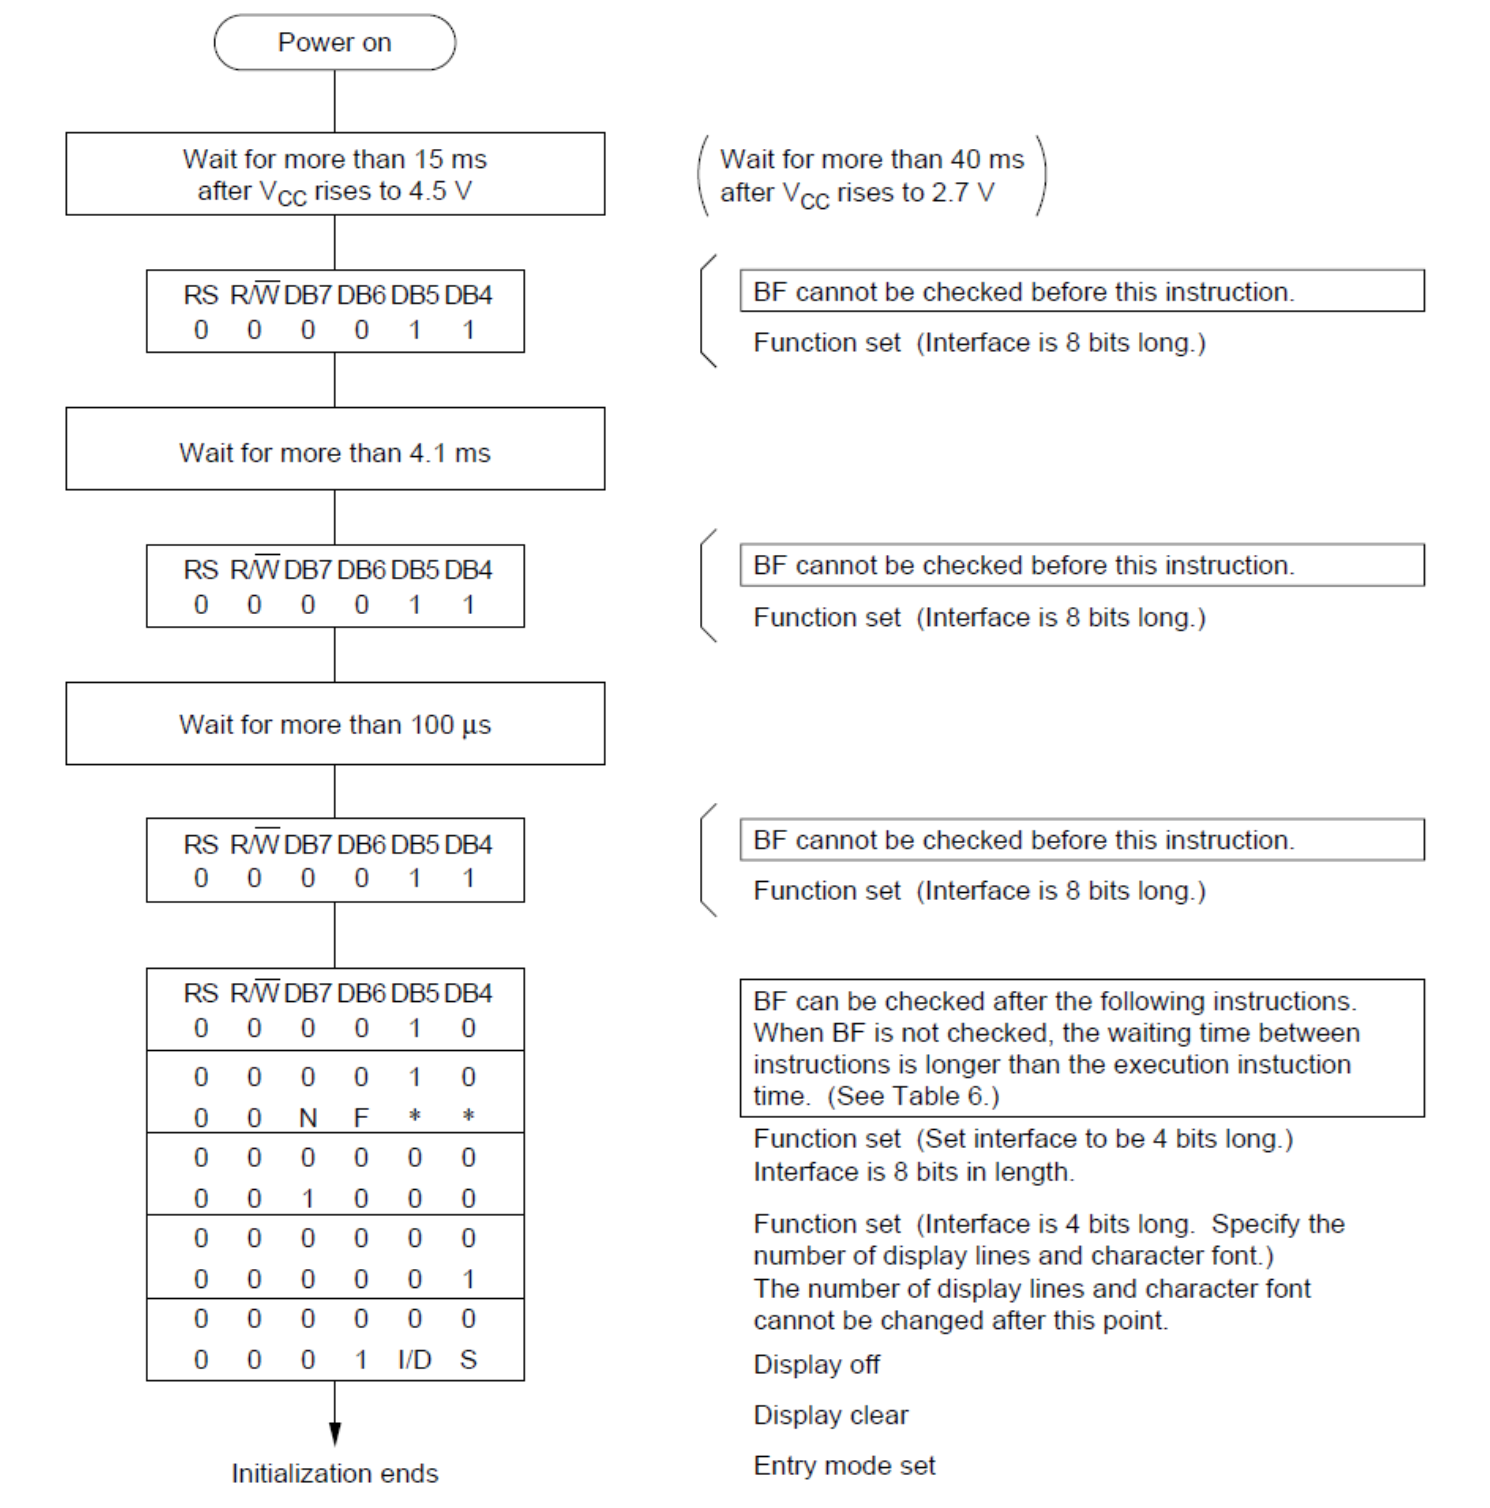
\includegraphics[keepaspectratio]{contents/core/img/chapter5-lcd-init.png}}

}

\caption{Figure 5.7: Block diagram of initialization sequence for
HD44780U in 4-bit mode (HD44780U Datasheet page 46)}

\end{figure}%

\subsection{LCD Wait}\label{lcd-wait}

The LCD's busy flag can be read while it processes commands internally.
To handle this, you can implement the \texttt{lcd\_wait} function, which
repeatedly reads the busy flag by setting R/W to 0 and configuring the
data lines as input. When the function should wait in a while loop
reading the busy flag until the LCD is again ready to accept commands.
Calling \texttt{lcd\_wait} should be done before sending any
instructions or data to the LCD, to ensure that it is ready to receive
data. Alternatively, you can use the \texttt{sl\_sleeptimer\_delay\_ms}
function to wait for a duration longer than any command processing
requires. While this latter approach is simpler, it is less effective
for high-frequency display updates due to the inherent required delay.
For this technique, waiting for 2 milliseconds following any command is
practical and easy to implement.

\subsection{Exercise: Displaying a centered
string}\label{exercise-displaying-a-centered-string}

For this exercise, write a function that writes a c-string argument
centered on the first line of the display. Check that the string passed
to the function is no longer than 16 characters. With this condition
met, calculate based on the length of the string the DDRAM address
offset necessary to center the string.

For example, the string \texttt{EE260} is \(5\) characters long. The
number of characters that should be blank on the line is \(16-5=11\). To
left align the text, the necessary offset is obviously \(0\). To right
align the text, the offset should be \(11\), so that the \(5\)
additional characters are placed directly touching the right side of the
display. To center align the text, the remaining blank characters must
be divided by 2. An integer division of \(11/2=5\) as the decimal is
truncated, meaning that the necessary DDRAM offset is \(5\), which will
leave \(6\) characters to the right of the text.

The necessary DDRAM offset may then be set using the appropriate LCD
command, then the characters of the string transferred to the display.

As an extension to this exercise, you may write a function that takes an
additional argument to select the type of alignment and display line to
place an arbitrary string of text on.

\section{Keypad}\label{keypad}

Many embedded systems with user interfaces are controlled by simple
inputs, such as a joystick, multifunctional knobs, or often, a group of
buttons. In cases where many buttons are required, such as for numerical
or even text input, connecting a single button to its own GPIO pin is
inefficient. With a 4x4 grid of buttons requiring 16 pins, an I/O
expander or separate microcontroller dedicated to I/O would likely be
necessary. However, a clever arrangement of switches in a grid such as
this allows for pins to be multiplexed, requiring a minimum of
\(\sqrt{\text{\# of buttons}}\) pins to read each button. This works by
connecting one side of each switch to a common row, and the other side
of the switch to a common column. For a 4x4 grid, only 8 pins are
necessary to read the entire matrix layout.

\subsection{Keypad Matrix Wiring}\label{keypad-matrix-wiring}

Commonly available matrix keypads simply implement the row and column
switch connections to pushbuttons integrated in the module. Their pinout
is often just a connection for each row and column, allowing them to
easily be connected to GPIO pins on an MCU, as shown in Figure
\hyperref[fig:keypadwiring]{5.8}.

The internal connections of the keypad may be displayed differently
depending on preferences for the schematic. However, it is common to see
the switches aligned on a 45angle, bridging between their respective row
and column common lines, as illustrated in Figure
\hyperref[fig:keypadschematic]{5.9}.

\begin{figure}[H]

{\centering \pandocbounded{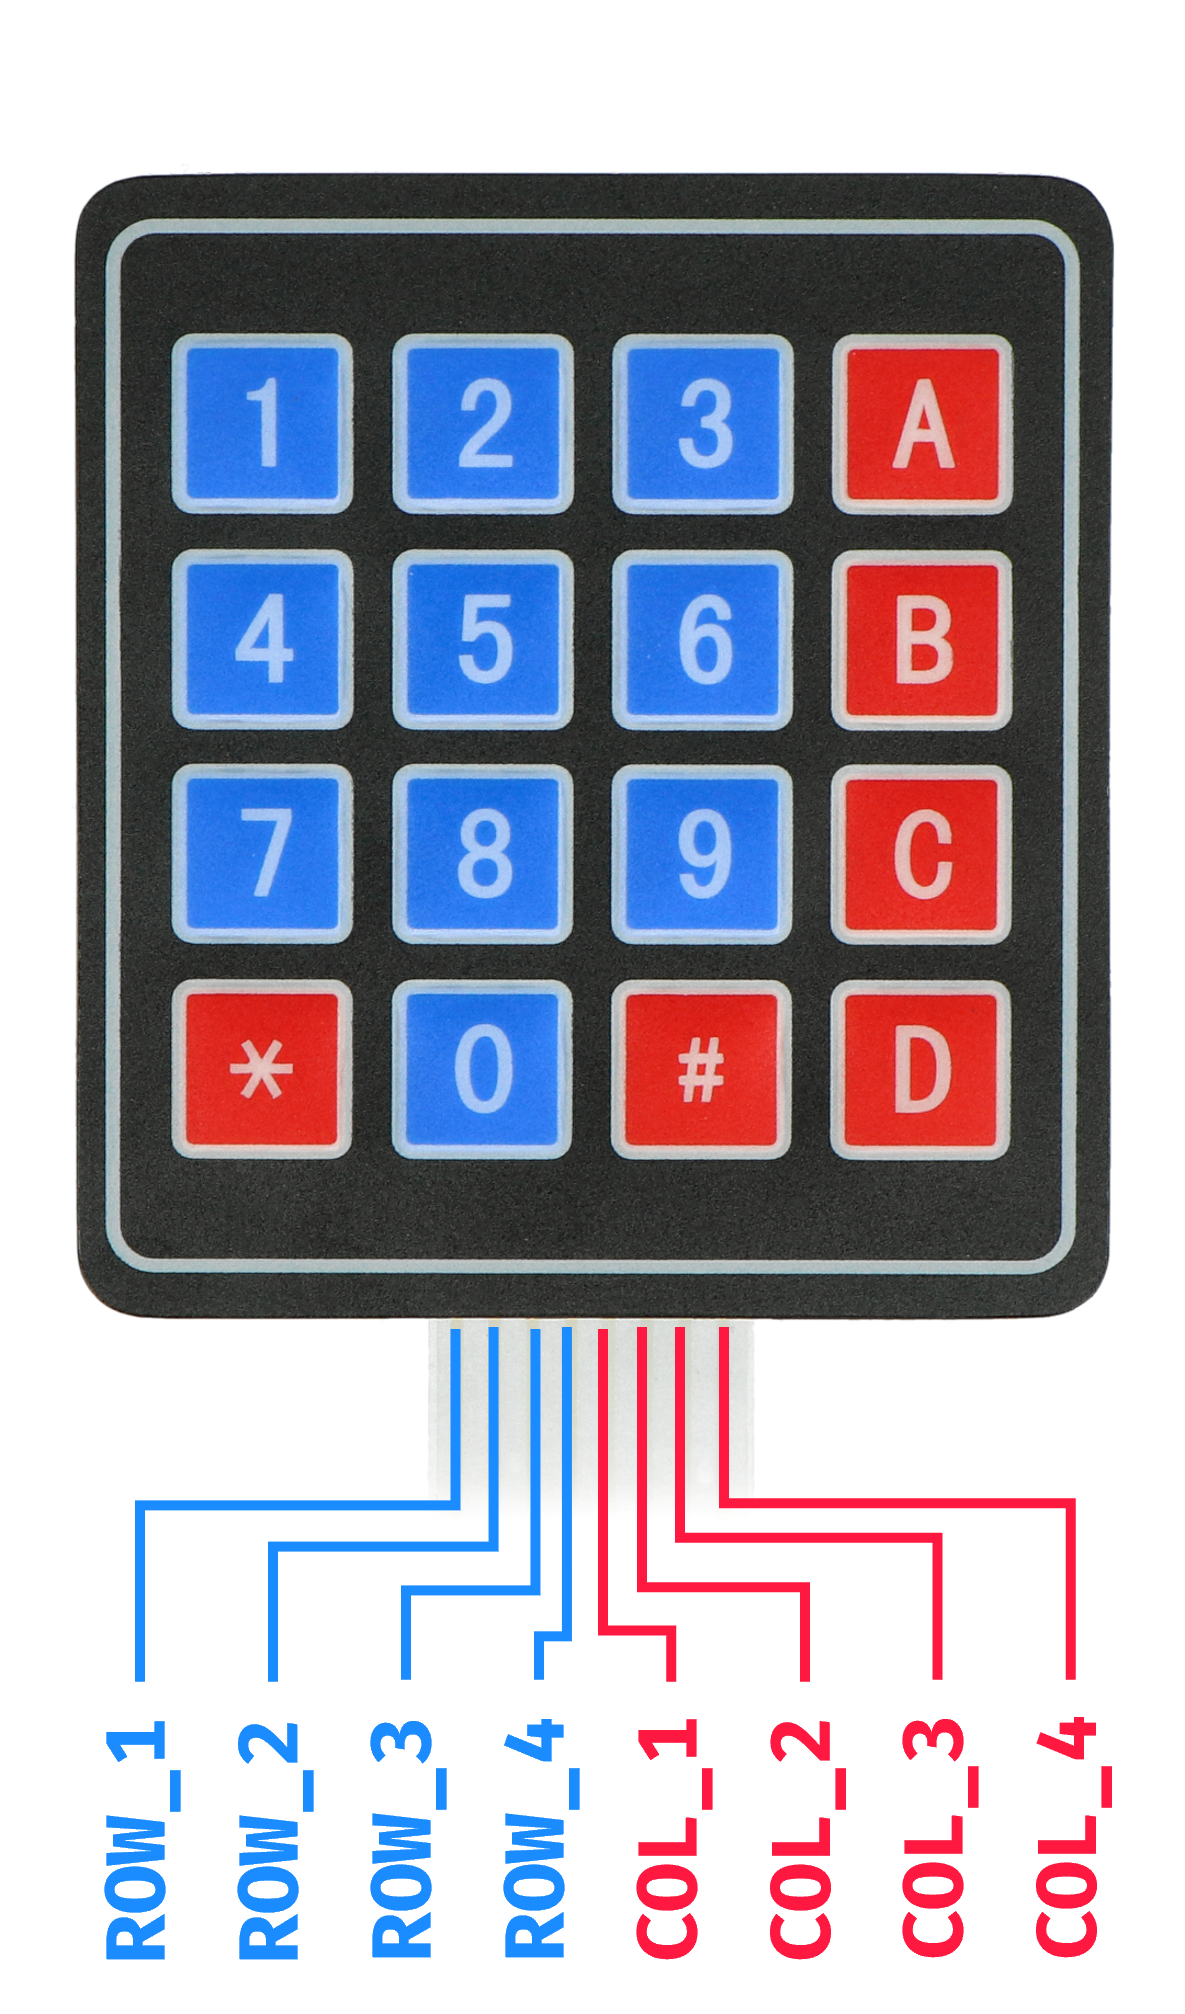
\includegraphics[keepaspectratio]{contents/core/img/chapter5-keypad-wiring.png}}

}

\caption{Figure 5.8: Pinout for an off-the-shelf keypad}

\end{figure}%%
\begin{figure}[H]

{\centering \pandocbounded{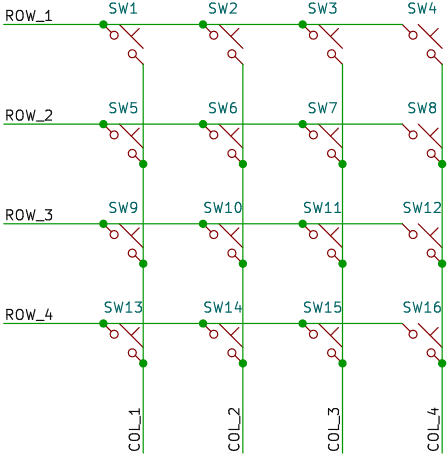
\includegraphics[keepaspectratio]{contents/core/img/chapter5-keypad-schematic.png}}

}

\caption{Figure 5.9: Schematic diagram of a 4x4 pushbutton switch
matrix}

\end{figure}%

\subsection{Reading Keypad Matrix}\label{reading-keypad-matrix}

To read a matrix of switches, one axis should be connected to GPIO
outputs. For example, we will connect the rows to output pins, writing
all pins high to begin with. The other axis should be connected to
internally pulled-down inputs, meaning that when any key is pressed, one
of the high rows will be connected to the input, bringing it high. When
this is detected, either with polling or an interrupt-based system, the
microcontroller may now identify which key has been pressed.

\subsection{Identifying Pressed Key}\label{identifying-pressed-key}

Once the MCU has been alerted that any key has been pressed, it may now
scan the switch matrix to determine the specific key. To do this, all
rows should be written low, except for the first row. This may be
achieved in practice by writing all rows low first, then immediately
writing the first row high. The MCU may then check if any key in the
first row has been pressed by again reading all of the column inputs. If
any of the column inputs are high, the currently checked row and column
that is high correspond with the pressed key. Otherwise, the MCU must
repeat the process, writing the next row low. In this way, the pressed
key can quickly be determined, and other actions can be taken based on
it. This process is outlined in Figure
\hyperref[fig:keypaddetectionflowchart]{5.10}, a flowchart showing the
logic necessary for efficient detection of keypresses.

\begin{figure}[H]

{\centering \pandocbounded{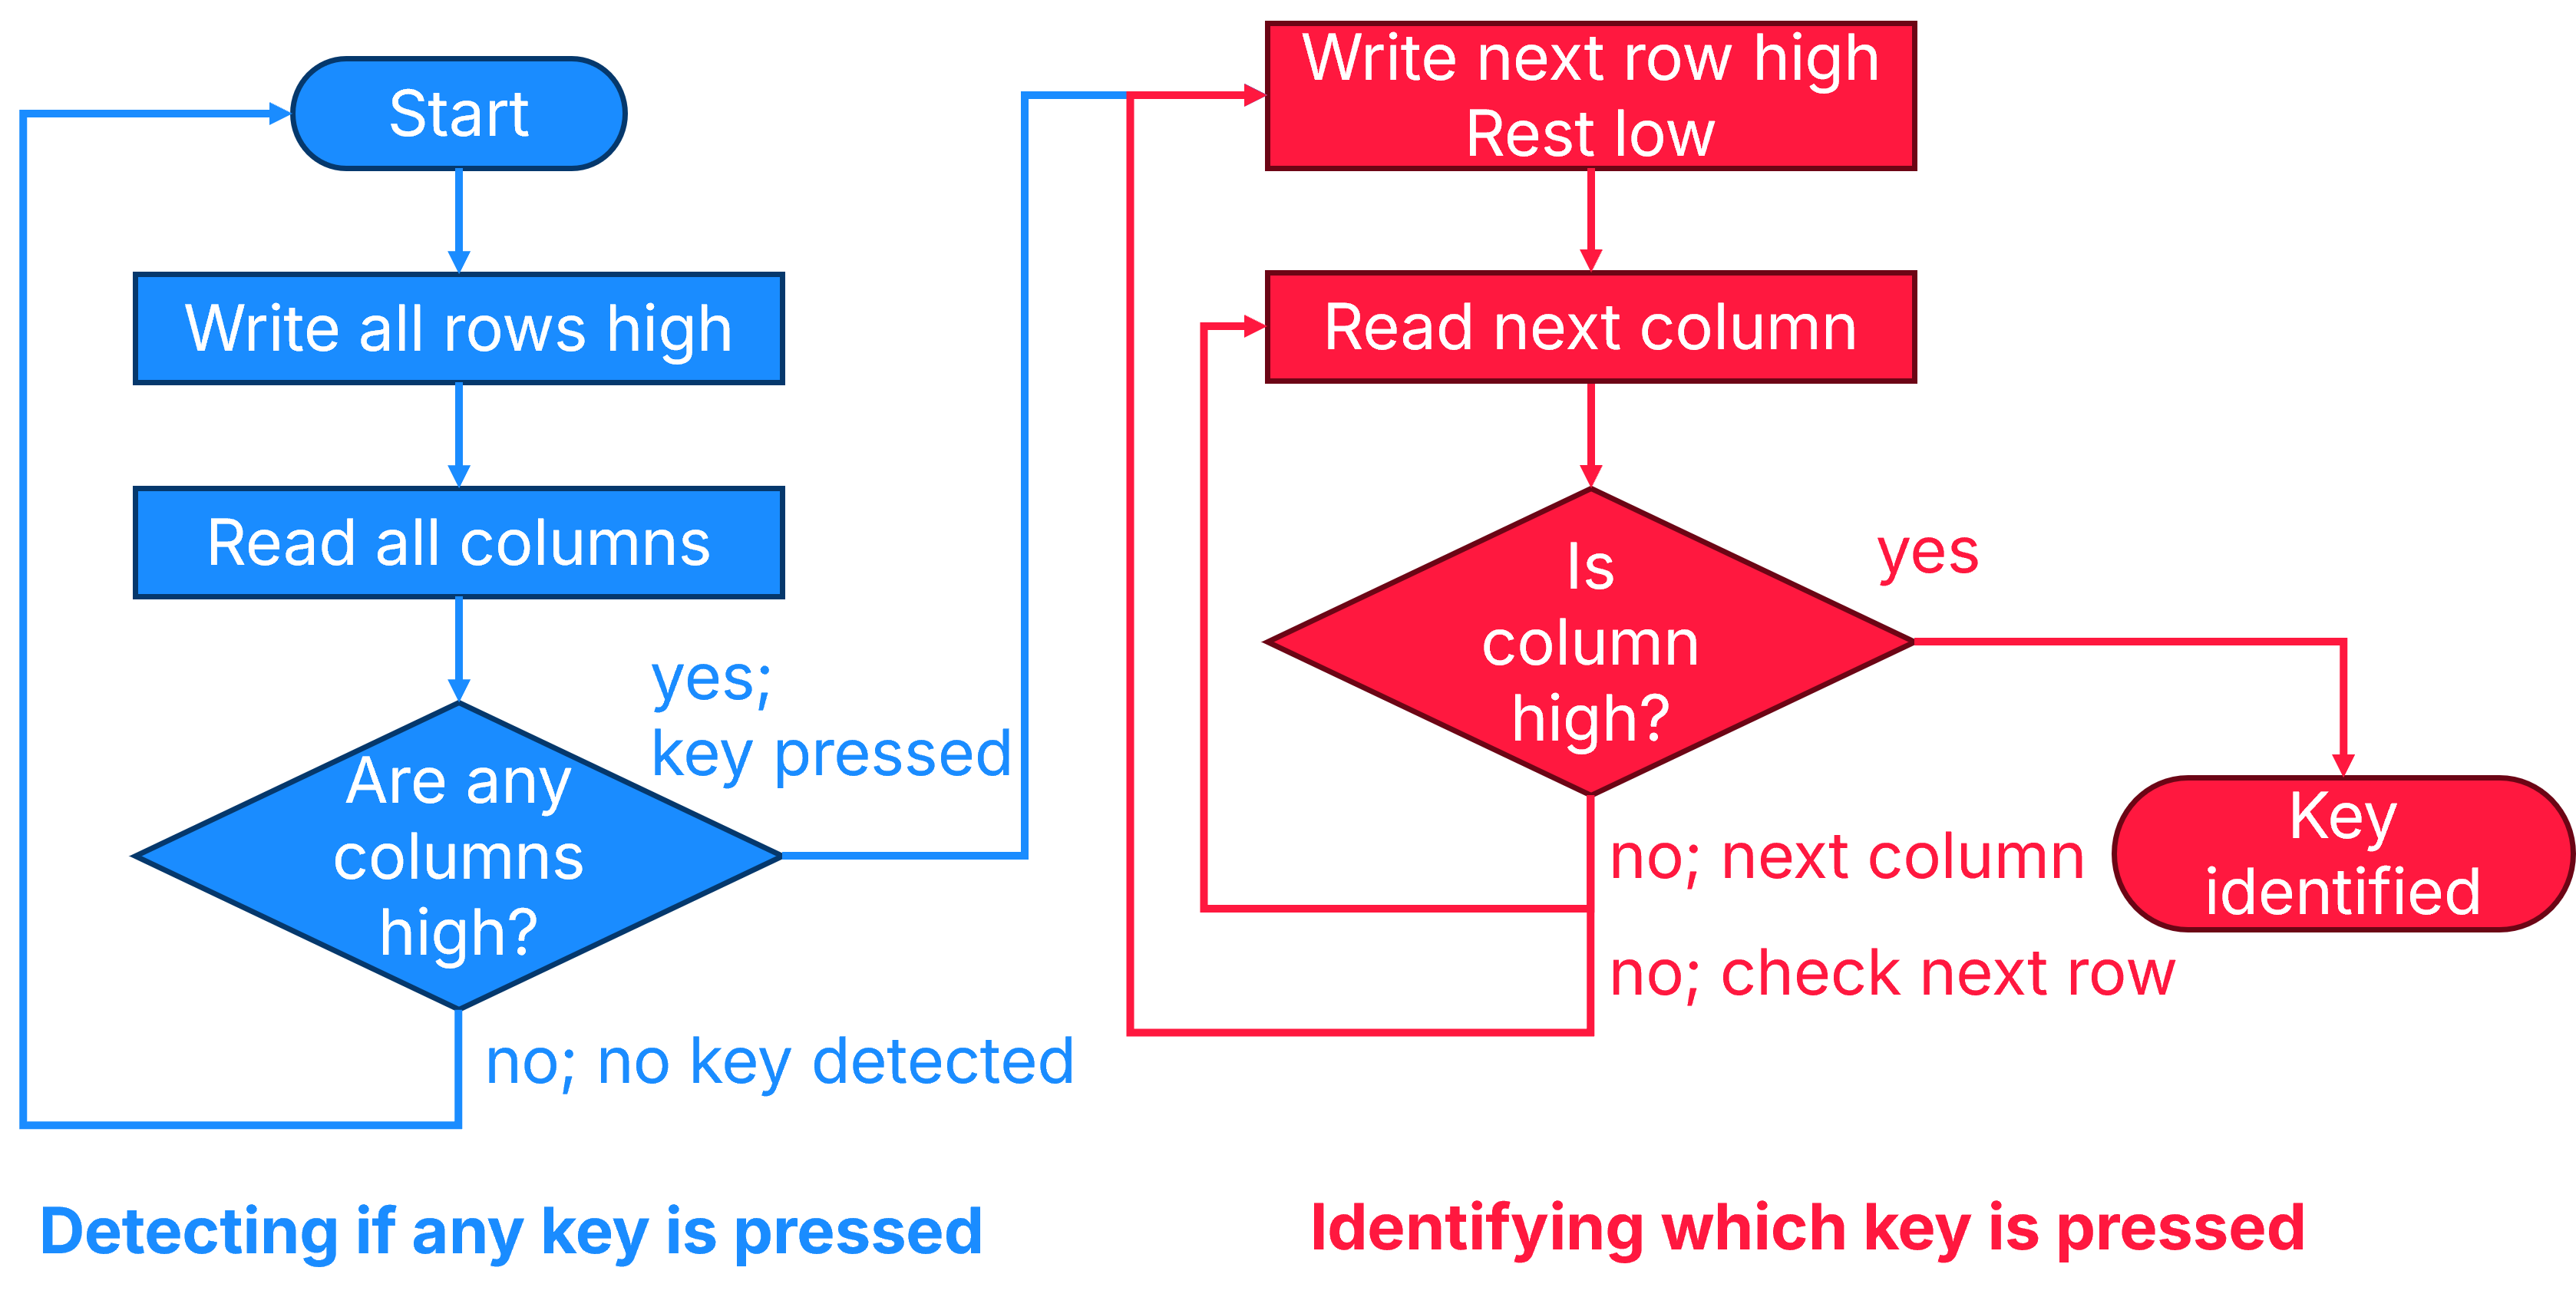
\includegraphics[keepaspectratio]{contents/core/img/chapter5-keypad-flowchart.png}}

}

\caption{Figure 5.10: Flowchart for detecting any keypress, then
identifying the speci ic key}

\end{figure}%

A simplified sample implementation of this process is included below.
The code implements nested-loop logic to scan a 4x4 matrix keypad using
EFR32XG24 Dev Kit GPIO pins. First, the GPIO pins are initialized, with
the column input pins (PC04--PC01) are configured as inputs, and the row
output pins (PC05, PA07--PA05) are set to push-pull (output) mode. In
the main loop, all the row pins are activated by setting them high.
Then, if any of the column pins detects a high signal, representing a
key press, the program iterates through each row to isolate the pressed
key. During this process, all rows are brought low save for the current
row of interest, and the program checks each column pin to identify the
specific key pressed.

\begin{Shaded}
\begin{Highlighting}[]
\CommentTok{// column inputs are on PC04{-}PC01}
\DataTypeTok{const} \DataTypeTok{uint8\_t}\NormalTok{ row\_ports}\OperatorTok{[]} \OperatorTok{=} \OperatorTok{\{}\DecValTok{2}\OperatorTok{,} \DecValTok{0}\OperatorTok{,} \DecValTok{0}\OperatorTok{,} \DecValTok{0}\OperatorTok{\};} \CommentTok{// PC05, PA07{-}PA05 are row outputs}
\DataTypeTok{const} \DataTypeTok{uint8\_t}\NormalTok{ row\_pins}\OperatorTok{[]} \OperatorTok{=} \OperatorTok{\{}\DecValTok{5}\OperatorTok{,} \DecValTok{7}\OperatorTok{,} \DecValTok{6}\OperatorTok{,} \DecValTok{5}\OperatorTok{\};}  \CommentTok{// PC05, PA07{-}PA05 are row outputs}

\DataTypeTok{int}\NormalTok{ main}\OperatorTok{(}\DataTypeTok{void}\OperatorTok{)}
\OperatorTok{\{}
\NormalTok{    GPIO}\OperatorTok{{-}\textgreater{}}\NormalTok{P}\OperatorTok{[}\NormalTok{gpioPortC}\OperatorTok{].}\NormalTok{MODEL }\OperatorTok{|=} \BaseNTok{0x1111} \OperatorTok{\textless{}\textless{}} \OperatorTok{(}\DecValTok{1} \OperatorTok{*} \DecValTok{4}\OperatorTok{);} \CommentTok{// input mode}

    \ControlFlowTok{for} \OperatorTok{(}\DataTypeTok{int}\NormalTok{ i }\OperatorTok{=} \DecValTok{0}\OperatorTok{;}\NormalTok{ i }\OperatorTok{\textless{}} \DecValTok{4}\OperatorTok{;}\NormalTok{ i}\OperatorTok{++)}
\NormalTok{        GPIO}\OperatorTok{{-}\textgreater{}}\NormalTok{P}\OperatorTok{[}\NormalTok{row\_ports}\OperatorTok{[}\NormalTok{i}\OperatorTok{]].}\NormalTok{MODEL }\OperatorTok{|=} \BaseNTok{0x4} \OperatorTok{\textless{}\textless{}} \OperatorTok{(}\NormalTok{row\_pins}\OperatorTok{[}\NormalTok{i}\OperatorTok{]} \OperatorTok{*} \DecValTok{4}\OperatorTok{);} \CommentTok{// output mode}

    \ControlFlowTok{while} \OperatorTok{(}\DecValTok{1}\OperatorTok{)}
    \OperatorTok{\{}
        \ControlFlowTok{for} \OperatorTok{(}\DataTypeTok{int}\NormalTok{ i }\OperatorTok{=} \DecValTok{0}\OperatorTok{;}\NormalTok{ i }\OperatorTok{\textless{}} \DecValTok{4}\OperatorTok{;}\NormalTok{ i}\OperatorTok{++)}
\NormalTok{            GPIO}\OperatorTok{{-}\textgreater{}}\NormalTok{P\_SET}\OperatorTok{[}\NormalTok{row\_ports}\OperatorTok{[}\NormalTok{i}\OperatorTok{]]} \OperatorTok{=} \DecValTok{1} \OperatorTok{\textless{}\textless{}}\NormalTok{ row\_pins}\OperatorTok{[}\NormalTok{i}\OperatorTok{];} \CommentTok{// set row pins}

        \ControlFlowTok{if} \OperatorTok{(}\NormalTok{GPIO}\OperatorTok{{-}\textgreater{}}\NormalTok{P}\OperatorTok{[}\NormalTok{gpioPortC}\OperatorTok{].}\NormalTok{DIN }\OperatorTok{\&} \BaseNTok{0xF} \OperatorTok{\textless{}\textless{}} \DecValTok{1}\OperatorTok{)} \CommentTok{// check if any key is pressed}
        \OperatorTok{\{}
            \ControlFlowTok{for} \OperatorTok{(}\DataTypeTok{int}\NormalTok{ i }\OperatorTok{=} \DecValTok{0}\OperatorTok{;}\NormalTok{ i }\OperatorTok{\textless{}} \DecValTok{4}\OperatorTok{;}\NormalTok{ i}\OperatorTok{++)} \CommentTok{// loop through all columns}
            \OperatorTok{\{}
                \ControlFlowTok{for} \OperatorTok{(}\DataTypeTok{int}\NormalTok{ j }\OperatorTok{=} \DecValTok{0}\OperatorTok{;}\NormalTok{ j }\OperatorTok{\textless{}} \DecValTok{4}\OperatorTok{;}\NormalTok{ j}\OperatorTok{++)}
\NormalTok{                    GPIO}\OperatorTok{{-}\textgreater{}}\NormalTok{P\_CLR}\OperatorTok{[}\NormalTok{row\_ports}\OperatorTok{[}\NormalTok{j}\OperatorTok{]]} \OperatorTok{=} \DecValTok{1} \OperatorTok{\textless{}\textless{}}\NormalTok{ row\_pins}\OperatorTok{[}\NormalTok{j}\OperatorTok{];} \CommentTok{// clear all row pins}
\NormalTok{                GPIO}\OperatorTok{{-}\textgreater{}}\NormalTok{P\_SET}\OperatorTok{[}\NormalTok{row\_ports}\OperatorTok{[}\NormalTok{i}\OperatorTok{]]} \OperatorTok{=} \DecValTok{1} \OperatorTok{\textless{}\textless{}}\NormalTok{ row\_pins}\OperatorTok{[}\NormalTok{i}\OperatorTok{];}     \CommentTok{// set current row pin}

                \ControlFlowTok{for} \OperatorTok{(}\DataTypeTok{int}\NormalTok{ i }\OperatorTok{=} \DecValTok{0}\OperatorTok{;}\NormalTok{ i }\OperatorTok{\textless{}} \DecValTok{4}\OperatorTok{;}\NormalTok{ i}\OperatorTok{++)}
                \OperatorTok{\{}
                    \ControlFlowTok{if} \OperatorTok{(}\NormalTok{GPIO}\OperatorTok{{-}\textgreater{}}\NormalTok{P}\OperatorTok{[}\NormalTok{gpioPortC}\OperatorTok{].}\NormalTok{DIN }\OperatorTok{\textless{}\textless{}} \DecValTok{1} \OperatorTok{\&} \DecValTok{1} \OperatorTok{\textless{}\textless{}}\NormalTok{ i}\OperatorTok{)} \CommentTok{// check if column pin is high}
                    \OperatorTok{\{}
                        \CommentTok{// this is the key pressed}
                    \OperatorTok{\}}
                \OperatorTok{\}}
            \OperatorTok{\}}
        \OperatorTok{\}}
    \OperatorTok{\}}
\OperatorTok{\}}
\end{Highlighting}
\end{Shaded}

\subsection{Power Efficiency}\label{power-efficiency}

A key benefit of reading a switch matrix using this technique,
especially with the EFR32MG24, which supports GPIO interrupts from all
Energy Management levels. This means that the processor may go into its
deepest sleep state while still waiting for keypresses from the matrix.
This requires interrupt logic, which will be discussed later, but the
general implementation is as follows:

The GPIO pins for the rows may be set high, and configured to retain
their values while in sleep mode. An interrupt to wake the processor
from sleep may be enabled on all input pins, meaning that any keypresses
will now trigger the interrupt, waking the MCU from sleep. It can now
progress directly into the key identification phase, finding the pressed
key and performing an action before returning to low-power sleep.

\subsection{Limitations of Switch
Matrix}\label{limitations-of-switch-matrix}

There exist a few limitations with this naive technique of reducing GPIO
pin usage for a switch matrix, the most significant being the lack of
\emph{key rollover}. This means that the MCU cannot identify multiple
keys being pressed, at least not with certainty.

Finally, if the keypress time is very short, a key pressed and caught by
the detection routine may already be released and missed by the
identification routine. This can be compounded by switch bouncing
because many keyboard matrices lack hardware debouncing, while software
debouncing requires keys to be pressed for a longer period of time
before the press is registered.

\subsection{Exercise: Propose a solution to the key rollover
problem}\label{exercise-propose-a-solution-to-the-key-rollover-problem}

Modern computer keyboards can detect any of their keys being pressed, as
well as any combination of keys being pressed. To do this, they do not
even require multiple I/O expanders or additional microcontrollers.
Instead, there is electronic hardware integrated into the matrix circuit
in series with every switch that ensures the proper key is detected.

What could this hardware be? Explain how it may be used to support
multiple simultaneous keypresses.

\part{Embedded Machine Learning}

\chapter{Real-Time Gesture
Recognition}\label{real-time-gesture-recognition}

Edge AI combines the power of artificial intelligence and edge computing
to enable real-time decision-making directly on embedded devices. This
chapter explores the implementation of Edge AI for gesture recognition
using the EFR32XG24 microcontroller. By leveraging AI models optimized
for resource-constrained environments, embedded systems can interpret
gesture inputs with low latency and high accuracy, enhancing
applications in fields such as human-computer interaction,
rehabilitation, and IoT-based control systems.

\section{Introduction to Edge AI in Embedded
Systems}\label{introduction-to-edge-ai-in-embedded-systems}

Edge AI refers to deploying AI models on edge devices, such as
microcontrollers, where data is processed locally instead of being sent
to a centralized cloud server. This paradigm reduces latency, enhances
data privacy, and ensures uninterrupted operation even in environments
with limited connectivity.

As embedded systems become more advanced, the need for efficient
on-device data processing grows. Traditional systems rely heavily on
cloud infrastructure, which can introduce latency, data privacy
concerns, and increased operational costs. Edge AI addresses these
issues by allowing computations to occur on the microcontroller itself,
ensuring responsiveness and independence from network stability. With
microcontrollers like the EFR32XG24, AI algorithms are executed
efficiently despite hardware and memory constraints.

\begin{Shaded}
\begin{Highlighting}[]
\CommentTok{// Example: Initialize Edge AI on EFR32XG24}
\DataTypeTok{void}\NormalTok{ initEdgeAI}\OperatorTok{()} \OperatorTok{\{}
\NormalTok{    configureClock}\OperatorTok{();}
\NormalTok{    enableAIAccelerator}\OperatorTok{();}
\NormalTok{    loadAIModel}\OperatorTok{();}
\NormalTok{    initializeSensors}\OperatorTok{();}
\OperatorTok{\}}

\NormalTok{initEdgeAI}\OperatorTok{();}
\end{Highlighting}
\end{Shaded}

\subsection{Advantages of Edge AI}\label{advantages-of-edge-ai}

Edge AI offers several critical advantages that make it an essential
technology for embedded systems:

\begin{itemize}
\item
  \textbf{Low Latency:} Immediate processing without reliance on cloud
  servers.
\item
  \textbf{Improved Privacy:} Sensitive data remains on the device.
\item
  \textbf{Reduced Bandwidth Usage:} No need for constant data
  transmission.
\item
  \textbf{Energy Efficiency:} Optimized AI models reduce power
  consumption.
\item
  \textbf{Scalability:} Multiple devices can operate independently.
\item
  \textbf{Offline Operation:} Systems continue functioning without an
  active internet connection.
\end{itemize}

These benefits are especially important in applications like gesture
recognition, where real-time response is crucial for effective
interaction. Devices deployed in remote or resource-limited environments
can operate reliably without relying on continuous cloud access.

\begin{Shaded}
\begin{Highlighting}[]
\CommentTok{// Example: Optimizing AI Model}
\DataTypeTok{void}\NormalTok{ optimizeAIModel}\OperatorTok{()} \OperatorTok{\{}
\NormalTok{    reducePrecision}\OperatorTok{();}
\NormalTok{    quantizeWeights}\OperatorTok{();}
\NormalTok{    minimizeMemoryFootprint}\OperatorTok{();}
\OperatorTok{\}}

\NormalTok{optimizeAIModel}\OperatorTok{();}
\end{Highlighting}
\end{Shaded}

\subsection{Why EFR32XG24 for Edge AI?}\label{why-efr32xg24-for-edge-ai}

The EFR32XG24 microcontroller, equipped with an ARM Cortex-M33 core and
integrated BLE capabilities, provides an ideal platform for Edge AI
applications. Its features include:

\begin{itemize}
\item
  Support for TinyML frameworks.
\item
  Dedicated hardware accelerators for AI computations.
\item
  Energy-efficient architecture for battery-operated devices.
\item
  Advanced security features for data integrity.
\item
  High-speed BLE communication for real-time data transfer.
\item
  Integrated peripherals for sensor interfacing.
\end{itemize}

\begin{Shaded}
\begin{Highlighting}[]
\CommentTok{// Example: BLE Initialization for Edge AI}
\DataTypeTok{void}\NormalTok{ initBLE}\OperatorTok{()} \OperatorTok{\{}
\NormalTok{    BLE\_init}\OperatorTok{();}
\NormalTok{    BLE\_enable}\OperatorTok{();}
\NormalTok{    BLE\_setMode}\OperatorTok{(}\NormalTok{BLE\_LOW\_POWER}\OperatorTok{);}
\OperatorTok{\}}

\NormalTok{initBLE}\OperatorTok{();}
\end{Highlighting}
\end{Shaded}

Furthermore, the microcontroller's native support for TensorFlow Lite
for Microcontrollers (TFLM) allows seamless deployment of lightweight AI
models. Its power efficiency ensures prolonged operational life.

\section{Gesture Recognition System
Overview}\label{gesture-recognition-system-overview}

Gesture recognition systems are a subset of human-computer interaction
technologies that allow users to control and interact with devices using
physical gestures. In an embedded context, gesture recognition systems
aim to interpret motion patterns captured by sensors like IMUs (Inertial
Measurement Units). The EFR32XG24 microcontroller enables real-time
gesture recognition while maintaining energy efficiency and
responsiveness.

\subsection{System Components}\label{system-components}

A gesture recognition system using the EFR32XG24 microcontroller
involves several key components:

\begin{itemize}
\item
  \textbf{Sensors:} Inertial Measurement Unit (IMU) for capturing motion
  data.
\item
  \textbf{AI Model:} A lightweight Convolutional Neural Network (CNN)
  optimized for TinyML.
\item
  \textbf{Data Preprocessing:} Noise filtering and segmentation.
\item
  \textbf{BLE Communication:} Real-time data transfer to mobile devices.
\item
  \textbf{Power Management System:} Ensures long battery life.
\end{itemize}

\begin{Shaded}
\begin{Highlighting}[]
\CommentTok{// Example: Read IMU Sensor Data}
\DataTypeTok{float}\NormalTok{ readIMU}\OperatorTok{()} \OperatorTok{\{}
    \DataTypeTok{float}\NormalTok{ x }\OperatorTok{=}\NormalTok{ IMU\_getX}\OperatorTok{();}
    \DataTypeTok{float}\NormalTok{ y }\OperatorTok{=}\NormalTok{ IMU\_getY}\OperatorTok{();}
    \DataTypeTok{float}\NormalTok{ z }\OperatorTok{=}\NormalTok{ IMU\_getZ}\OperatorTok{();}
    \ControlFlowTok{return} \OperatorTok{(}\NormalTok{x }\OperatorTok{+}\NormalTok{ y }\OperatorTok{+}\NormalTok{ z}\OperatorTok{)} \OperatorTok{/} \DecValTok{3}\OperatorTok{;}
\OperatorTok{\}}
\end{Highlighting}
\end{Shaded}

\subsection{System Workflow}\label{system-workflow}

The overall workflow of a gesture recognition system includes the
following stages:

\begin{enumerate}
\def\labelenumi{\arabic{enumi}.}
\item
  Raw sensor data is captured using IMU sensors.
\item
  Data is preprocessed locally to remove noise.
\item
  Preprocessed data is fed into the AI model.
\item
  The AI model classifies the gesture.
\item
  Results are sent via BLE to a connected device.
\item
  Feedback is displayed in real-time on a mobile or desktop application.
\end{enumerate}

\section{AI Model Design for Gesture
Recognition}\label{ai-model-design-for-gesture-recognition}

The AI model for gesture recognition is implemented using a
TinyML-compatible CNN architecture.

\subsection{Model Architecture}\label{model-architecture}

The CNN architecture is carefully designed to balance accuracy, memory
consumption, and computational efficiency:

\begin{itemize}
\item
  \textbf{Input Layer:} Processes time-series IMU data.
\item
  \textbf{Convolutional Layers:} Extract spatial and temporal patterns.
\item
  \textbf{Dropout Layers:} Prevent overfitting.
\item
  \textbf{Fully Connected Layer:} Classifies gestures.
\item
  \textbf{Softmax Layer:} Provides final classification probabilities.
\end{itemize}

\begin{Shaded}
\begin{Highlighting}[]
\CommentTok{// Example: Preprocessing IMU Data}
\DataTypeTok{void}\NormalTok{ preprocessIMUData}\OperatorTok{(}\DataTypeTok{float}\OperatorTok{*}\NormalTok{ data}\OperatorTok{,} \DataTypeTok{int}\NormalTok{ size}\OperatorTok{)} \OperatorTok{\{}
    \ControlFlowTok{for} \OperatorTok{(}\DataTypeTok{int}\NormalTok{ i }\OperatorTok{=} \DecValTok{0}\OperatorTok{;}\NormalTok{ i }\OperatorTok{\textless{}}\NormalTok{ size}\OperatorTok{;}\NormalTok{ i}\OperatorTok{++)} \OperatorTok{\{}
\NormalTok{        data}\OperatorTok{[}\NormalTok{i}\OperatorTok{]} \OperatorTok{=}\NormalTok{ normalize}\OperatorTok{(}\NormalTok{data}\OperatorTok{[}\NormalTok{i}\OperatorTok{]);}
    \OperatorTok{\}}
\OperatorTok{\}}
\end{Highlighting}
\end{Shaded}

\begin{longtable}[]{@{}lll@{}}
\toprule\noalign{}
\textbf{Layer} & \textbf{Type} & \textbf{Output Shape} \\
\midrule\noalign{}
\endfirsthead
\toprule\noalign{}
\textbf{Layer} & \textbf{Type} & \textbf{Output Shape} \\
\midrule\noalign{}
\endhead
\bottomrule\noalign{}
\tabularnewline
\caption{Table 6.1: AI Model Layers and Parameters}\tabularnewline
\endlastfoot
Input & Time-Series Data & (128, 3, 1) \\
Conv2D & Feature Extraction & (64, 128, 3, 8) \\
MaxPooling2D & Downsampling & (32, 64, 8) \\
Dropout & Regularization & - \\
Flatten & Vectorization & (512) \\
Dense & Classification & (16) \\
Output & Softmax & (4) \\
\end{longtable}

\section{Methodology}\label{sec:methodology}

This section outlines the methodology used to design and implement an
Edge AI-based gesture recognition system on the EFR32XG24 BLE
microcontroller. The methodology consists of four main stages: Data
Acquisition, Data Preprocessing, AI Model Development, and System
Integration. Each stage is elaborated below.

\subsection{Data Acquisition}\label{data-acquisition}

The gesture recognition system utilizes an Inertial Measurement Unit
(IMU) sensor to capture motion data. The IMU consists of accelerometers,
gyroscopes, and magnetometers to measure linear acceleration, angular
velocity, and orientation, respectively.

\textbf{Sensor Configuration:}

\begin{itemize}
\item
  \textbf{Sensor Type:} 6-axis IMU sensor.
\item
  \textbf{Sampling Rate:} 50 Hz.
\item
  \textbf{Data Format:} Time-series data with X, Y, and Z-axis readings.
\end{itemize}

The IMU sensor outputs raw motion data, which is collected in real-time
and fed into the microcontroller for preprocessing.

\subsection{Data Preprocessing}\label{data-preprocessing}

Raw data from the IMU sensor is noisy and requires preprocessing before
being fed into the AI model. The preprocessing pipeline includes the
following steps:

\begin{enumerate}
\def\labelenumi{\arabic{enumi}.}
\item
  \textbf{Noise Filtering:} A low-pass filter is applied to remove
  high-frequency noise.
\item
  \textbf{Normalization:} Sensor readings are normalized to a common
  scale between 0 and 1.
\item
  \textbf{Segmentation:} The data is divided into fixed-size time
  windows for analysis.
\end{enumerate}

The preprocessed data ensures consistency and reduces variability,
enabling robust AI model performance.

\subsection{AI Model Development}\label{ai-model-development}

The AI model is implemented using a TinyML-compatible Convolutional
Neural Network (CNN). The architecture is optimized for low memory and
computational constraints typical of embedded devices.

\textbf{Model Architecture:}

\begin{itemize}
\item
  \textbf{Input Layer:} Accepts preprocessed IMU time-series data.
\item
  \textbf{Convolutional Layers:} Extract spatial and temporal patterns.
\item
  \textbf{Pooling Layers:} Reduce dimensionality while retaining
  critical features.
\item
  \textbf{Dropout Layers:} Prevent overfitting during training.
\item
  \textbf{Fully Connected Layers:} Map learned features to output
  classes.
\item
  \textbf{Output Layer:} Softmax layer providing probabilities for each
  gesture class.
\end{itemize}

\textbf{Training and Optimization:}

\begin{itemize}
\item
  \textbf{Framework:} TensorFlow Lite for Microcontrollers (TFLM).
\item
  \textbf{Training Dataset:} Recorded gesture datasets.
\item
  \textbf{Optimization Techniques:} Weight quantization, reduced
  precision arithmetic, and model pruning.
\end{itemize}

The model was trained offline on a high-performance server and deployed
onto the EFR32XG24 microcontroller after optimization.

\subsection{System Integration}\label{system-integration}

The final deployment involves integrating the AI model with the
EFR32XG24 microcontroller and establishing BLE communication for data
transfer and feedback display.

\textbf{System Workflow:}

\begin{enumerate}
\def\labelenumi{\arabic{enumi}.}
\item
  IMU sensors capture real-time motion data.
\item
  Data preprocessing is performed locally on the microcontroller.
\item
  The preprocessed data is passed to the AI model for gesture
  classification.
\item
  Results are transmitted via BLE to connected mobile or desktop
  applications.
\item
  Feedback is displayed in real-time.
\end{enumerate}

\textbf{Power Management:}

\begin{itemize}
\item
  Adaptive power management is implemented to minimize battery
  consumption.
\item
  Low-power BLE mode is enabled for data transmission.
\end{itemize}

\subsection{Evaluation Metrics}\label{evaluation-metrics}

The system's performance was evaluated using the following metrics:

\begin{itemize}
\item
  \textbf{Accuracy:} Percentage of correct gesture classifications.
\item
  \textbf{Latency:} Time taken for end-to-end gesture recognition.
\item
  \textbf{Power Consumption:} Average energy used per gesture
  recognition cycle.
\end{itemize}

\subsection{Hardware and Software
Tools}\label{hardware-and-software-tools}

\begin{itemize}
\item
  \textbf{Hardware:} EFR32XG24 BLE microcontroller, IMU sensor module.
\item
  \textbf{Software:} TensorFlow Lite for Microcontrollers, Embedded C,
  BLE SDK.
\end{itemize}

The methodology ensures an efficient, real-time, and scalable gesture
recognition system optimized for embedded hardware constraints.

\section{Challenges and Limitations}\label{sec:challenges}

While implementing the Edge AI-based gesture recognition system on the
EFR32XG24 microcontroller, several challenges and limitations were
encountered. These are discussed below:

\begin{enumerate}
\def\labelenumi{\arabic{enumi}.}
\item
  \textbf{Hardware Constraints:} The limited computational power and
  memory resources of the microcontroller posed restrictions on the
  complexity and size of the AI model. Optimizing the AI model for
  memory efficiency while maintaining accuracy was a significant
  challenge.
\item
  \textbf{Power Consumption:} Real-time gesture recognition is
  computationally intensive, and ensuring prolonged battery life for
  portable devices required careful power management strategies.
\item
  \textbf{Sensor Noise:} IMU sensors are susceptible to noise and
  environmental disturbances, which can introduce inaccuracies in
  gesture data. Filtering and preprocessing techniques had to be
  carefully designed to address this issue.
\item
  \textbf{Latency Constraints:} Edge AI systems require minimal latency
  for real-time performance. Achieving low latency while balancing model
  accuracy and computational load was challenging.
\item
  \textbf{BLE Communication Bottlenecks:} Real-time data transfer via
  BLE can be affected by interference, limited bandwidth, and power
  constraints, impacting system responsiveness.
\item
  \textbf{Scalability:**} Scaling the system for multi-gesture
  recognition or increasing the number of edge devices posed integration
  challenges due to resource limitations.
\item
  \textbf{Environmental Variability:} Gesture recognition accuracy can
  degrade under varying environmental conditions, such as lighting
  changes, device orientation, or sudden movements.
\end{enumerate}

Addressing these challenges required a combination of hardware
optimization, software fine-tuning, and iterative testing to ensure a
balance between performance, accuracy, and efficiency.

\chapter{\texorpdfstring{\textbf{Magic Wand via Gesture
Recognition}}{Magic Wand via Gesture Recognition}}\label{magic-wand-via-gesture-recognition}

The EFR32xG24 board has high capabilities for edge computing necessary
for capturing, processing, and analyzing data in real time with improved
security and reduced latency. The Magic Wand with BLE Gesture
Recognition (BLE-MW) is an ideal project to exemplify this concept
through the implementation of a TinyML classifier for gesture
recognition. It incorporates a quantized TinyML, accelerometer data
processing of the onboard IMU, and a BLE communication protocol. The
project files are available at
\href{https://github.com/Ijnaka22len/ble_magic_wand}{\texttt{github.com/Ijnaka22len/ble\_magic\_wand}},
following the original implementation in
\href{https://github.com/SiliconLabs/machine_learning_applications/tree/main/application/imu/ble_magic_wand}{\texttt{github.com/SiliconLabs/machine\_learning\_applications}}.

\section{System Overview}\label{system-overview}

A convolutional neural network (CNN) model was trained in this TinyML
project to recognize gestures such as Swipe Up, Swipe Down, and Circle
based on the onboard accelerometer data. The detected gestures (Arrow
Up, Arrow Down, and Play/Pause) are mapped to media control actions and
transmitted over BLE as media key presses and over the UART interface.
Figure~\hyperref[fig:output_instance]{7.1} shows an instance of the
output.

\begin{figure}[H]

{\centering \pandocbounded{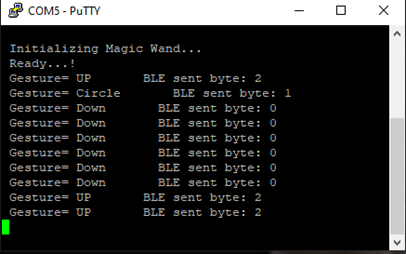
\includegraphics[keepaspectratio]{contents/core/img/chapter7-uart-output.png}}

}

\caption{Figure 7.1: Sample Data Output via UART Terminal}

\end{figure}%

\section{Data Collection and
Processing}\label{data-collection-and-processing}

The IMU data for this TinyML model was collected at 25Hz with a sequence
length of 50 samples to form the input buffer for the CNN. The fastest
way to do this is by following the
\texttt{github.com/Ijnaka22len/FastDataCollection4MagicWangProjects}
repository, which provides a detailed description of IMU data capture
for TinyML projects. The captured data is preprocessed and fed into the
model as an input image for pattern recognition.

\begin{Shaded}
\begin{Highlighting}[]
\ControlFlowTok{if}\NormalTok{ \_\_name\_\_ }\OperatorTok{==} \StringTok{"\_\_main\_\_"}\OperatorTok{:}
\NormalTok{    delFile}\OperatorTok{(}\NormalTok{file\_path}\OperatorTok{=}\StringTok{"data/complete\_data"}\OperatorTok{)}
\NormalTok{    delFile}\OperatorTok{(}\NormalTok{file\_path}\OperatorTok{=}\StringTok{"data/test"}\OperatorTok{)}
\NormalTok{    delFile}\OperatorTok{(}\NormalTok{file\_path}\OperatorTok{=}\StringTok{"data/train"}\OperatorTok{)}
\NormalTok{    delFile}\OperatorTok{(}\NormalTok{file\_path}\OperatorTok{=}\StringTok{"data/valid"}\OperatorTok{)}
\NormalTok{    delFile}\OperatorTok{(}\NormalTok{file\_path}\OperatorTok{=}\StringTok{"netmodels/CNN/weights.h5"}\OperatorTok{)}

\NormalTok{    folders }\OperatorTok{=}\NormalTok{ os}\OperatorTok{.}\NormalTok{listdir}\OperatorTok{(}\StringTok{"data"}\OperatorTok{)}
\NormalTok{    names }\OperatorTok{=} \OperatorTok{[}\NormalTok{file}\OperatorTok{.}\NormalTok{split}\OperatorTok{(}\CharTok{\textquotesingle{}\_\textquotesingle{}}\OperatorTok{)[}\DecValTok{1}\OperatorTok{].}\NormalTok{lower}\OperatorTok{()} \ControlFlowTok{for}\NormalTok{ file in os}\OperatorTok{.}\NormalTok{listdir}\OperatorTok{(}\NormalTok{f}\StringTok{"data/\{folders[0]\}"}\OperatorTok{)]}
\NormalTok{    data }\OperatorTok{=} \OperatorTok{[]}\NormalTok{  \# pylint}\OperatorTok{:}\NormalTok{ disable}\OperatorTok{=}\NormalTok{redefined}\OperatorTok{{-}}\NormalTok{outer}\OperatorTok{{-}}\NormalTok{name}

    \ControlFlowTok{for}\NormalTok{ idx1}\OperatorTok{,}\NormalTok{ folder in enumerate}\OperatorTok{(}\NormalTok{folders}\OperatorTok{):}
\NormalTok{        files }\OperatorTok{=}\NormalTok{ os}\OperatorTok{.}\NormalTok{listdir}\OperatorTok{(}\NormalTok{f}\StringTok{"data/\{folder\}"}\OperatorTok{)}
        \ControlFlowTok{for}\NormalTok{ file in files}\OperatorTok{:}
\NormalTok{            name }\OperatorTok{=}\NormalTok{ file}\OperatorTok{.}\NormalTok{split}\OperatorTok{(}\CharTok{\textquotesingle{}\_\textquotesingle{}}\OperatorTok{)[}\DecValTok{1}\OperatorTok{].}\NormalTok{lower}\OperatorTok{()}
\NormalTok{            prepare\_original\_data}\OperatorTok{(}\NormalTok{folder}\OperatorTok{,}\NormalTok{ name}\OperatorTok{,}\NormalTok{ data}\OperatorTok{,}\NormalTok{ f}\StringTok{"data/\{folder\}/\{file\}"}\OperatorTok{)}

    \ControlFlowTok{for}\NormalTok{ idx in range}\OperatorTok{(}\DecValTok{5}\OperatorTok{):}
\NormalTok{        prepare\_original\_data}\OperatorTok{(}\StringTok{"negative"}\OperatorTok{,} \StringTok{"negative}\SpecialCharTok{\%d}\StringTok{"} \OperatorTok{\%} \OperatorTok{(}\NormalTok{idx }\OperatorTok{+} \DecValTok{1}\OperatorTok{),}\NormalTok{ data}\OperatorTok{,} \StringTok{"data/negative/negative\_}\SpecialCharTok{\%d}\StringTok{.txt"} \OperatorTok{\%} \OperatorTok{(}\NormalTok{idx }\OperatorTok{+} \DecValTok{1}\OperatorTok{))}
    
\NormalTok{    generate\_negative\_data}\OperatorTok{(}\NormalTok{data}\OperatorTok{)}
\NormalTok{    print}\OperatorTok{(}\StringTok{"data\_length: "} \OperatorTok{+}\NormalTok{ str}\OperatorTok{(}\NormalTok{len}\OperatorTok{(}\NormalTok{data}\OperatorTok{)))}

    \ControlFlowTok{if}\NormalTok{ not os}\OperatorTok{.}\NormalTok{path}\OperatorTok{.}\NormalTok{exists}\OperatorTok{(}\StringTok{"./data"}\OperatorTok{):}
\NormalTok{        os}\OperatorTok{.}\NormalTok{makedirs}\OperatorTok{(}\StringTok{"./data"}\OperatorTok{)}
    
\NormalTok{    write\_data}\OperatorTok{(}\NormalTok{data}\OperatorTok{,} \StringTok{"./data/complete\_data"}\OperatorTok{)}
\end{Highlighting}
\end{Shaded}

\section{Model Architecture and
Deployment}\label{model-architecture-and-deployment}

TensorFlow Lite is used to create the CNN model, which takes the
processed IMU data as an input image for multiclass classification of
the various classes. The AIDrawPen chapter can be reviewed to show how
to train a TinyML model for this microcontroller.

\begin{Shaded}
\begin{Highlighting}[]
\StringTok{"""Trains the model."""}
\NormalTok{calculate\_model\_size}\OperatorTok{(}\NormalTok{model}\OperatorTok{)}
\NormalTok{epochs }\OperatorTok{=} \DecValTok{50}
\NormalTok{batch\_size }\OperatorTok{=} \DecValTok{64}
\NormalTok{model}\OperatorTok{.}\NormalTok{compile}\OperatorTok{(}\NormalTok{optimizer}\OperatorTok{=}\StringTok{"adam"}\OperatorTok{,}
\NormalTok{              loss}\OperatorTok{=}\StringTok{"sparse\_categorical\_crossentropy"}\OperatorTok{,}
\NormalTok{              metrics}\OperatorTok{=[}\StringTok{"accuracy"}\OperatorTok{])}
\ControlFlowTok{if}\NormalTok{ kind }\OperatorTok{==} \StringTok{"CNN"}\OperatorTok{:}
\NormalTok{    train\_data }\OperatorTok{=}\NormalTok{ train\_data}\OperatorTok{.}\NormalTok{map}\OperatorTok{(}\NormalTok{reshape\_function}\OperatorTok{)}
\NormalTok{    test\_data }\OperatorTok{=}\NormalTok{ test\_data}\OperatorTok{.}\NormalTok{map}\OperatorTok{(}\NormalTok{reshape\_function}\OperatorTok{)}
\NormalTok{    valid\_data }\OperatorTok{=}\NormalTok{ valid\_data}\OperatorTok{.}\NormalTok{map}\OperatorTok{(}\NormalTok{reshape\_function}\OperatorTok{)}

\NormalTok{test\_labels }\OperatorTok{=}\NormalTok{ np}\OperatorTok{.}\NormalTok{zeros}\OperatorTok{(}\NormalTok{test\_len}\OperatorTok{)}
\NormalTok{idx }\OperatorTok{=} \DecValTok{0}
\ControlFlowTok{for}\NormalTok{ data}\OperatorTok{,}\NormalTok{ label in test\_data}\OperatorTok{:}\NormalTok{  \# pylint}\OperatorTok{:}\NormalTok{ disable}\OperatorTok{=}\NormalTok{unused}\OperatorTok{{-}}\NormalTok{variable}
\NormalTok{    test\_labels}\OperatorTok{[}\NormalTok{idx}\OperatorTok{]} \OperatorTok{=}\NormalTok{ label}\OperatorTok{.}\NormalTok{numpy}\OperatorTok{()}
\NormalTok{    idx }\OperatorTok{+=} \DecValTok{1}

\NormalTok{train\_data }\OperatorTok{=}\NormalTok{ train\_data}\OperatorTok{.}\NormalTok{batch}\OperatorTok{(}\NormalTok{batch\_size}\OperatorTok{).}\NormalTok{repeat}\OperatorTok{()}
\NormalTok{valid\_data }\OperatorTok{=}\NormalTok{ valid\_data}\OperatorTok{.}\NormalTok{batch}\OperatorTok{(}\NormalTok{batch\_size}\OperatorTok{)}
\NormalTok{test\_data }\OperatorTok{=}\NormalTok{ test\_data}\OperatorTok{.}\NormalTok{batch}\OperatorTok{(}\NormalTok{batch\_size}\OperatorTok{)}

\NormalTok{history }\OperatorTok{=}\NormalTok{ model}\OperatorTok{.}\NormalTok{fit}\OperatorTok{(}\NormalTok{train\_data}\OperatorTok{,}
\NormalTok{              epochs}\OperatorTok{=}\NormalTok{epochs}\OperatorTok{,}
\NormalTok{              validation\_data}\OperatorTok{=}\NormalTok{valid\_data}\OperatorTok{,}
\NormalTok{              steps\_per\_epoch}\OperatorTok{=}\DecValTok{1000}\OperatorTok{,}
\NormalTok{              validation\_steps}\OperatorTok{=}\DataTypeTok{int}\OperatorTok{((}\NormalTok{valid\_len }\OperatorTok{{-}} \DecValTok{1}\OperatorTok{)} \OperatorTok{/}\NormalTok{ batch\_size }\OperatorTok{+} \DecValTok{1}\OperatorTok{),}
\NormalTok{              callbacks}\OperatorTok{=[}\NormalTok{tensorboard\_callback}\OperatorTok{,}\NormalTok{ early\_stop}\OperatorTok{,}\NormalTok{ checkpoint}\OperatorTok{])}

\NormalTok{loss}\OperatorTok{,}\NormalTok{ acc }\OperatorTok{=}\NormalTok{ model}\OperatorTok{.}\NormalTok{evaluate}\OperatorTok{(}\NormalTok{test\_data}\OperatorTok{)}
\NormalTok{pred }\OperatorTok{=}\NormalTok{ np}\OperatorTok{.}\NormalTok{argmax}\OperatorTok{(}\NormalTok{model}\OperatorTok{.}\NormalTok{predict}\OperatorTok{(}\NormalTok{test\_data}\OperatorTok{),}\NormalTok{ axis}\OperatorTok{=}\DecValTok{1}\OperatorTok{)}
\NormalTok{confusion }\OperatorTok{=}\NormalTok{ tf}\OperatorTok{.}\NormalTok{math}\OperatorTok{.}\NormalTok{confusion\_matrix}\OperatorTok{(}\NormalTok{labels}\OperatorTok{=}\NormalTok{tf}\OperatorTok{.}\NormalTok{constant}\OperatorTok{(}\NormalTok{test\_labels}\OperatorTok{),}
\NormalTok{                                     predictions}\OperatorTok{=}\NormalTok{tf}\OperatorTok{.}\NormalTok{constant}\OperatorTok{(}\NormalTok{pred}\OperatorTok{),}
\NormalTok{                                     num\_classes}\OperatorTok{=}\DecValTok{4}\OperatorTok{)}
\end{Highlighting}
\end{Shaded}

\section{Firmware and Model
Inference}\label{firmware-and-model-inference}

The microcontroller firmware contains a code segment to capture the
accelerometer data at the predetermined frequency and sampling rate.
This data is stored in a buffer and updated every 100ms during gesture
detection.

\begin{Shaded}
\begin{Highlighting}[]
\PreprocessorTok{\#include }\ImportTok{"accelerometer.h"}
\PreprocessorTok{\#include }\ImportTok{"config.h"}

\PreprocessorTok{\#if defined(SL\_COMPONENT\_CATALOG\_PRESENT)}
\PreprocessorTok{\#include }\ImportTok{"sl\_component\_catalog.h"}
\PreprocessorTok{\#endif}

\PreprocessorTok{\#if defined (SL\_CATALOG\_ICM20689\_DRIVER\_PRESENT)}
\PreprocessorTok{\#include }\ImportTok{"sl\_icm20689\_config.h"}
\PreprocessorTok{\#define  SL\_IMU\_INT\_PORT SL\_ICM20689\_INT\_PORT}
\PreprocessorTok{\#define  SL\_IMU\_INT\_PIN  SL\_ICM20689\_INT\_PIN}
\PreprocessorTok{\#elif defined (SL\_CATALOG\_ICM20648\_DRIVER\_PRESENT)}
\PreprocessorTok{\#include }\ImportTok{"sl\_icm20648\_config.h"}
\PreprocessorTok{\#define  SL\_IMU\_INT\_PORT SL\_ICM20648\_INT\_PORT}
\PreprocessorTok{\#define  SL\_IMU\_INT\_PIN  SL\_ICM20648\_INT\_PIN}
\PreprocessorTok{\#else}
\PreprocessorTok{\#error "No IMU driver defined"}
\PreprocessorTok{\#endif}

\CommentTok{// Accelerometer data from sensor}
\KeywordTok{typedef} \KeywordTok{struct}\NormalTok{ imu\_data }\OperatorTok{\{}
  \DataTypeTok{int16\_t}\NormalTok{ x}\OperatorTok{;}
  \DataTypeTok{int16\_t}\NormalTok{ y}\OperatorTok{;}
  \DataTypeTok{int16\_t}\NormalTok{ z}\OperatorTok{;}
\OperatorTok{\}}\NormalTok{ imu\_data\_t}\OperatorTok{;}

\NormalTok{sl\_status\_t accelerometer\_setup}\OperatorTok{(}\NormalTok{GPIOINT\_IrqCallbackPtrExt\_t callbackPtr}\OperatorTok{)}
\OperatorTok{\{}
\NormalTok{  sl\_status\_t status }\OperatorTok{=}\NormalTok{ SL\_STATUS\_OK}\OperatorTok{;}
  \DataTypeTok{int}\NormalTok{ int\_id}\OperatorTok{;}

  \CommentTok{// Initialize accelerometer sensor}
\NormalTok{  status }\OperatorTok{=}\NormalTok{ sl\_imu\_init}\OperatorTok{();}
  \ControlFlowTok{if} \OperatorTok{(}\NormalTok{status }\OperatorTok{!=}\NormalTok{ SL\_STATUS\_OK}\OperatorTok{)} \OperatorTok{\{}
    \ControlFlowTok{return}\NormalTok{ status}\OperatorTok{;}
  \OperatorTok{\}}
\NormalTok{  sl\_imu\_configure}\OperatorTok{(}\NormalTok{ACCELEROMETER\_FREQ}\OperatorTok{);}
  \CommentTok{// Setup interrupt from accelerometer on falling edge}
\NormalTok{  GPIO\_PinModeSet}\OperatorTok{(}\NormalTok{SL\_IMU\_INT\_PORT}\OperatorTok{,}\NormalTok{ SL\_IMU\_INT\_PIN}\OperatorTok{,}\NormalTok{ gpioModeInput}\OperatorTok{,} \DecValTok{0}\OperatorTok{);}
\NormalTok{  int\_id }\OperatorTok{=}\NormalTok{ GPIOINT\_CallbackRegisterExt}\OperatorTok{(}\NormalTok{SL\_IMU\_INT\_PIN}\OperatorTok{,}\NormalTok{ callbackPtr}\OperatorTok{,} \DecValTok{0}\OperatorTok{);}
  \ControlFlowTok{if} \OperatorTok{(}\NormalTok{int\_id }\OperatorTok{!=}\NormalTok{ INTERRUPT\_UNAVAILABLE}\OperatorTok{)} \OperatorTok{\{}
\NormalTok{    GPIO\_ExtIntConfig}\OperatorTok{(}\NormalTok{SL\_IMU\_INT\_PORT}\OperatorTok{,}\NormalTok{ SL\_IMU\_INT\_PIN}\OperatorTok{,}\NormalTok{ int\_id}\OperatorTok{,} \KeywordTok{false}\OperatorTok{,} \KeywordTok{true}\OperatorTok{,} \KeywordTok{true}\OperatorTok{);}
  \OperatorTok{\}} \ControlFlowTok{else} \OperatorTok{\{}
\NormalTok{    status }\OperatorTok{=}\NormalTok{ SL\_STATUS\_FAIL}\OperatorTok{;}
  \OperatorTok{\}}
  \ControlFlowTok{return}\NormalTok{ status}\OperatorTok{;}
\OperatorTok{\}}

\NormalTok{sl\_status\_t accelerometer\_read}\OperatorTok{(}\NormalTok{acc\_data\_t}\OperatorTok{*}\NormalTok{ dst}\OperatorTok{)}
\OperatorTok{\{}
  \ControlFlowTok{if} \OperatorTok{(!}\NormalTok{sl\_imu\_is\_data\_ready}\OperatorTok{())} \OperatorTok{\{}
    \ControlFlowTok{return}\NormalTok{ SL\_STATUS\_FAIL}\OperatorTok{;}
  \OperatorTok{\}}
\NormalTok{  sl\_imu\_update}\OperatorTok{();}
  \DataTypeTok{int16\_t}\NormalTok{ m}\OperatorTok{[}\DecValTok{3}\OperatorTok{];}
\NormalTok{  sl\_imu\_get\_acceleration}\OperatorTok{(}\NormalTok{m}\OperatorTok{);}
\NormalTok{  CORE\_DECLARE\_IRQ\_STATE}\OperatorTok{;}
\NormalTok{  CORE\_ENTER\_CRITICAL}\OperatorTok{();}
  \ControlFlowTok{if} \OperatorTok{(}\NormalTok{dst }\OperatorTok{!=}\NormalTok{ NULL}\OperatorTok{)} \OperatorTok{\{}
\NormalTok{    dst}\OperatorTok{{-}\textgreater{}}\NormalTok{x }\OperatorTok{=}\NormalTok{ m}\OperatorTok{[}\DecValTok{0}\OperatorTok{];}
\NormalTok{    dst}\OperatorTok{{-}\textgreater{}}\NormalTok{y }\OperatorTok{=}\NormalTok{ m}\OperatorTok{[}\DecValTok{1}\OperatorTok{];}
\NormalTok{    dst}\OperatorTok{{-}\textgreater{}}\NormalTok{z }\OperatorTok{=}\NormalTok{ m}\OperatorTok{[}\DecValTok{2}\OperatorTok{];}
  \OperatorTok{\}}
\NormalTok{  CORE\_EXIT\_CRITICAL}\OperatorTok{();}
  \ControlFlowTok{return}\NormalTok{ SL\_STATUS\_OK}\OperatorTok{;}
\OperatorTok{\}}
\end{Highlighting}
\end{Shaded}

The quantized CNN model interprets the processed accelerometer data to
classify gestures through periodic inference. Results are evaluated
against the accepted threshold (\#define DETECTION\_THRESHOLD 0.9f).

\begin{Shaded}
\begin{Highlighting}[]
\PreprocessorTok{\#include }\ImportTok{"sl\_tflite\_micro\_model.h"}
\PreprocessorTok{\#include }\ImportTok{"sl\_tflite\_micro\_init.h"}
\PreprocessorTok{\#include }\ImportTok{"sl\_sleeptimer.h"}
\PreprocessorTok{\#include }\ImportTok{"magic\_wand.h"}
\PreprocessorTok{\#include }\ImportTok{"accelerometer.h"}
\PreprocessorTok{\#include }\ImportTok{"sl\_simple\_button\_instances.h"}
\PreprocessorTok{\#include }\ImportTok{"math.h"}
\PreprocessorTok{\#include }\ImportTok{"config.h"}
\CommentTok{// BLE header}
\PreprocessorTok{\#include }\ImportTok{"sl\_bluetooth.h"}
\PreprocessorTok{\#include }\ImportTok{"app\_assert.h"}
\PreprocessorTok{\#include }\ImportTok{"gatt\_db.h"}
\PreprocessorTok{\#include }\ImportTok{"em\_common.h"}
\CommentTok{//}
\DataTypeTok{static} \DataTypeTok{int}\NormalTok{ input\_length}\OperatorTok{;}
\DataTypeTok{static}\NormalTok{ TfLiteTensor}\OperatorTok{*}\NormalTok{ model\_input}\OperatorTok{;}
\DataTypeTok{static}\NormalTok{ tflite}\OperatorTok{::}\NormalTok{MicroInterpreter}\OperatorTok{*}\NormalTok{ interpreter}\OperatorTok{;}
\DataTypeTok{static}\NormalTok{ acc\_data\_t buf}\OperatorTok{[}\NormalTok{SEQUENCE\_LENGTH}\OperatorTok{]} \OperatorTok{=} \OperatorTok{\{} \FloatTok{0.5}\BuiltInTok{f}\OperatorTok{,} \FloatTok{0.5}\BuiltInTok{f}\OperatorTok{,} \FloatTok{0.5}\BuiltInTok{f} \OperatorTok{\};}
\DataTypeTok{static} \DataTypeTok{bool}\NormalTok{ infer }\OperatorTok{=} \KeywordTok{false}\OperatorTok{;}
\DataTypeTok{static} \DataTypeTok{bool}\NormalTok{ read\_accel }\OperatorTok{=} \KeywordTok{false}\OperatorTok{;}
\DataTypeTok{static} \DataTypeTok{int}\NormalTok{ head\_ptr }\OperatorTok{=} \DecValTok{0}\OperatorTok{;}
\DataTypeTok{static} \DataTypeTok{int}\NormalTok{ inference\_trigger\_samples\_num }\OperatorTok{=}\NormalTok{ round}\OperatorTok{(}\NormalTok{INFERENCE\_PERIOD\_MS }\OperatorTok{/}\NormalTok{ ACCELEROMETER\_FREQ}\OperatorTok{);}
\DataTypeTok{static}\NormalTok{ acc\_data\_t prev\_data }\OperatorTok{=} \OperatorTok{\{} \FloatTok{0.5}\BuiltInTok{f}\OperatorTok{,} \FloatTok{0.5}\BuiltInTok{f}\OperatorTok{,} \FloatTok{0.5}\BuiltInTok{f} \OperatorTok{\};}

\DataTypeTok{static} \DataTypeTok{void}\NormalTok{ listen\_for\_gestures}\OperatorTok{(}\DataTypeTok{bool}\NormalTok{ enable}\OperatorTok{)}
\OperatorTok{\{}
  \ControlFlowTok{if} \OperatorTok{(}\NormalTok{enable}\OperatorTok{)} \OperatorTok{\{}
    \ControlFlowTok{for} \OperatorTok{(}\DataTypeTok{uint8\_t}\NormalTok{ i }\OperatorTok{=} \DecValTok{0}\OperatorTok{;}\NormalTok{ i }\OperatorTok{\textless{}}\NormalTok{ SEQUENCE\_LENGTH}\OperatorTok{;}\NormalTok{ i}\OperatorTok{++)} \OperatorTok{\{}
\NormalTok{      acc\_data\_t \_d }\OperatorTok{=} \OperatorTok{\{} \FloatTok{0.5}\BuiltInTok{f}\OperatorTok{,} \FloatTok{0.5}\BuiltInTok{f}\OperatorTok{,} \FloatTok{0.5}\BuiltInTok{f} \OperatorTok{\};}
\NormalTok{      buf}\OperatorTok{[}\NormalTok{i}\OperatorTok{]} \OperatorTok{=}\NormalTok{ \_d}\OperatorTok{;}
    \OperatorTok{\}}
\NormalTok{    read\_accel }\OperatorTok{=} \KeywordTok{true}\OperatorTok{;}
  \OperatorTok{\}} \ControlFlowTok{else} \OperatorTok{\{}
\NormalTok{    read\_accel }\OperatorTok{=} \KeywordTok{false}\OperatorTok{;}
\NormalTok{    head\_ptr }\OperatorTok{=} \DecValTok{0}\OperatorTok{;}
  \OperatorTok{\}}
\OperatorTok{\}}

\DataTypeTok{void}\NormalTok{ sl\_button\_on\_change}\OperatorTok{(}\DataTypeTok{const}\NormalTok{ sl\_button\_t }\OperatorTok{*}\NormalTok{handle}\OperatorTok{)}
\OperatorTok{\{}
  \ControlFlowTok{if} \OperatorTok{(}\NormalTok{sl\_button\_get\_state}\OperatorTok{(}\NormalTok{handle}\OperatorTok{)} \OperatorTok{==}\NormalTok{ SL\_SIMPLE\_BUTTON\_PRESSED}\OperatorTok{)} \OperatorTok{\{}
    \ControlFlowTok{if} \OperatorTok{(\&}\NormalTok{sl\_button\_btn0 }\OperatorTok{==}\NormalTok{ handle}\OperatorTok{)} \OperatorTok{\{}
\NormalTok{      listen\_for\_gestures}\OperatorTok{(}\KeywordTok{true}\OperatorTok{);}
    \OperatorTok{\}}
  \OperatorTok{\}} \ControlFlowTok{else} \ControlFlowTok{if} \OperatorTok{(}\NormalTok{sl\_button\_get\_state}\OperatorTok{(}\NormalTok{handle}\OperatorTok{)} \OperatorTok{==}\NormalTok{ SL\_SIMPLE\_BUTTON\_RELEASED}\OperatorTok{)} \OperatorTok{\{}
    \ControlFlowTok{if} \OperatorTok{(\&}\NormalTok{sl\_button\_btn0 }\OperatorTok{==}\NormalTok{ handle}\OperatorTok{)} \OperatorTok{\{}
\NormalTok{      listen\_for\_gestures}\OperatorTok{(}\KeywordTok{false}\OperatorTok{);}
    \OperatorTok{\}}
  \OperatorTok{\}}
\OperatorTok{\}}

\CommentTok{// Called when the IMU has data available using gpio interrupt.}
\DataTypeTok{static} \DataTypeTok{void}\NormalTok{ on\_data\_available}\OperatorTok{(}\DataTypeTok{uint8\_t}\NormalTok{ int\_id}\OperatorTok{,} \DataTypeTok{void} \OperatorTok{*}\NormalTok{ctx}\OperatorTok{)}
\OperatorTok{\{}
  \OperatorTok{(}\DataTypeTok{void}\OperatorTok{)}\NormalTok{ int\_id}\OperatorTok{;}
  \OperatorTok{(}\DataTypeTok{void}\OperatorTok{)}\NormalTok{ ctx}\OperatorTok{;}
\NormalTok{  acc\_data\_t data }\OperatorTok{=} \OperatorTok{\{} \DecValTok{0}\OperatorTok{,} \DecValTok{0}\OperatorTok{,} \DecValTok{0} \OperatorTok{\};}
\NormalTok{  sl\_status\_t status }\OperatorTok{=}\NormalTok{ accelerometer\_read}\OperatorTok{(\&}\NormalTok{data}\OperatorTok{);}
  \ControlFlowTok{if} \OperatorTok{(}\NormalTok{status }\OperatorTok{==}\NormalTok{ SL\_STATUS\_FAIL }\OperatorTok{||} \OperatorTok{!}\NormalTok{read\_accel}\OperatorTok{)} \OperatorTok{\{}
    \ControlFlowTok{return}\OperatorTok{;}
  \OperatorTok{\}}

\NormalTok{  data}\OperatorTok{.}\NormalTok{x }\OperatorTok{/=} \DecValTok{2000}\OperatorTok{;}
\NormalTok{  data}\OperatorTok{.}\NormalTok{y }\OperatorTok{/=} \DecValTok{2000}\OperatorTok{;}
\NormalTok{  data}\OperatorTok{.}\NormalTok{z }\OperatorTok{/=} \DecValTok{2000}\OperatorTok{;}

\NormalTok{  acc\_data\_t delta\_data }\OperatorTok{=} \OperatorTok{\{} \DecValTok{0} \OperatorTok{\};}
\NormalTok{  delta\_data}\OperatorTok{.}\NormalTok{x }\OperatorTok{=}\NormalTok{ data}\OperatorTok{.}\NormalTok{x }\OperatorTok{{-}}\NormalTok{ prev\_data}\OperatorTok{.}\NormalTok{x}\OperatorTok{;}
\NormalTok{  delta\_data}\OperatorTok{.}\NormalTok{y }\OperatorTok{=}\NormalTok{ data}\OperatorTok{.}\NormalTok{y }\OperatorTok{{-}}\NormalTok{ prev\_data}\OperatorTok{.}\NormalTok{y}\OperatorTok{;}
\NormalTok{  delta\_data}\OperatorTok{.}\NormalTok{z }\OperatorTok{=}\NormalTok{ data}\OperatorTok{.}\NormalTok{z }\OperatorTok{{-}}\NormalTok{ prev\_data}\OperatorTok{.}\NormalTok{z}\OperatorTok{;}

\NormalTok{  delta\_data}\OperatorTok{.}\NormalTok{x }\OperatorTok{=} \OperatorTok{(}\NormalTok{delta\_data}\OperatorTok{.}\NormalTok{x }\OperatorTok{/} \DecValTok{2} \OperatorTok{+} \DecValTok{1}\OperatorTok{)} \OperatorTok{/} \DecValTok{2}\OperatorTok{;}
\NormalTok{  delta\_data}\OperatorTok{.}\NormalTok{y }\OperatorTok{=} \OperatorTok{(}\NormalTok{delta\_data}\OperatorTok{.}\NormalTok{y }\OperatorTok{/} \DecValTok{2} \OperatorTok{+} \DecValTok{1}\OperatorTok{)} \OperatorTok{/} \DecValTok{2}\OperatorTok{;}
\NormalTok{  delta\_data}\OperatorTok{.}\NormalTok{z }\OperatorTok{=} \OperatorTok{(}\NormalTok{delta\_data}\OperatorTok{.}\NormalTok{z }\OperatorTok{/} \DecValTok{2} \OperatorTok{+} \DecValTok{1}\OperatorTok{)} \OperatorTok{/} \DecValTok{2}\OperatorTok{;}

\NormalTok{  buf}\OperatorTok{[}\NormalTok{head\_ptr}\OperatorTok{].}\NormalTok{x }\OperatorTok{=}\NormalTok{ delta\_data}\OperatorTok{.}\NormalTok{x}\OperatorTok{;}
\NormalTok{  buf}\OperatorTok{[}\NormalTok{head\_ptr}\OperatorTok{].}\NormalTok{y }\OperatorTok{=}\NormalTok{ delta\_data}\OperatorTok{.}\NormalTok{y}\OperatorTok{;}
\NormalTok{  buf}\OperatorTok{[}\NormalTok{head\_ptr}\OperatorTok{].}\NormalTok{z }\OperatorTok{=}\NormalTok{ delta\_data}\OperatorTok{.}\NormalTok{z}\OperatorTok{;}

\NormalTok{  head\_ptr}\OperatorTok{++;}
\NormalTok{  prev\_data}\OperatorTok{.}\NormalTok{x }\OperatorTok{=}\NormalTok{ data}\OperatorTok{.}\NormalTok{x}\OperatorTok{;}
\NormalTok{  prev\_data}\OperatorTok{.}\NormalTok{y }\OperatorTok{=}\NormalTok{ data}\OperatorTok{.}\NormalTok{y}\OperatorTok{;}
\NormalTok{  prev\_data}\OperatorTok{.}\NormalTok{z }\OperatorTok{=}\NormalTok{ data}\OperatorTok{.}\NormalTok{z}\OperatorTok{;}
  \ControlFlowTok{if} \OperatorTok{(}\NormalTok{head\_ptr }\OperatorTok{\textgreater{}=}\NormalTok{ SEQUENCE\_LENGTH}\OperatorTok{)} \OperatorTok{\{}
\NormalTok{    head\_ptr }\OperatorTok{=} \DecValTok{0}\OperatorTok{;}
  \OperatorTok{\}}
  \ControlFlowTok{if} \OperatorTok{(}\NormalTok{head\_ptr }\OperatorTok{\%}\NormalTok{ inference\_trigger\_samples\_num }\OperatorTok{==} \DecValTok{0}\OperatorTok{)} \OperatorTok{\{}
\NormalTok{    infer }\OperatorTok{=} \KeywordTok{true}\OperatorTok{;}
  \OperatorTok{\}}
\OperatorTok{\}}
\end{Highlighting}
\end{Shaded}

\section{Data Transfer and BLE
Communication}\label{data-transfer-and-ble-communication}

Predicted data is transferred through BLE using the GATT server as well
as logged to the Putty terminal.

\begin{Shaded}
\begin{Highlighting}[]
\DataTypeTok{void}\NormalTok{ send\_gesture\_via\_ble}\OperatorTok{(}\DataTypeTok{uint8\_t}\NormalTok{ gesture}\OperatorTok{)}
\OperatorTok{\{}
\NormalTok{    printf}\OperatorTok{(}\StringTok{" BLE sent byte: }\SpecialCharTok{\%u\textbackslash{}r\textbackslash{}n}\StringTok{"}\OperatorTok{,} \OperatorTok{(}\DataTypeTok{unsigned} \DataTypeTok{int}\OperatorTok{)}\NormalTok{gesture}\OperatorTok{);}
\NormalTok{    sl\_status\_t sc}\OperatorTok{;}
\NormalTok{    sc }\OperatorTok{=}\NormalTok{ sl\_bt\_gatt\_server\_notify\_all}\OperatorTok{(}\NormalTok{gattdb\_gesture\_data}\OperatorTok{,}
                                        \KeywordTok{sizeof}\OperatorTok{(}\NormalTok{gesture}\OperatorTok{),}
                                        \OperatorTok{\&}\NormalTok{gesture}\OperatorTok{);}
\NormalTok{    app\_assert\_status}\OperatorTok{(}\NormalTok{sc}\OperatorTok{);}
\OperatorTok{\}}
\end{Highlighting}
\end{Shaded}

\chapter{\texorpdfstring{\textbf{IMU Anomaly Detection Using
Hierarchical Temporal
Memory}}{IMU Anomaly Detection Using Hierarchical Temporal Memory}}\label{imu-anomaly-detection-using-hierarchical-temporal-memory}

Analyzing sensor data to identify rare or suspicious events, items or
observation that differ significantly from standard patterns. This
process is called anomaly detection, which is highly important in
product production. This chapter demonstrates the identification of
anomalies in real-time accelerometer data using the Hierarchical
Temporal Memory (HTM) algorithms. This project aims to show how edge
computing can be used to provide sensitive anomaly detection for diverse
applications such as machinery monitoring, motion analysis, and
safety-critical systems. The project files are available at
\href{https://github.com/Ijnaka22len/imu_anomaly_detection}{\texttt{github.com/Ijnaka22len/imu\_anomaly\_detection}},
following the original implementation in
\href{https://github.com/SiliconLabs/machine_learning_applications/tree/main/application/imu/imu_anomaly_detection}{\texttt{github.com/SiliconLabs/machine\_learning\_applications}}.

\section{System Overview}\label{system-overview-1}

Hierarchical Temporal Memory (HTM) is an algorithm that mimics the
brain's neocortical learning mechanisms and constantly learns time-based
patterns in unlabeled data. Anomalies (suspicious data) are flagged when
data (IMU data) deviate significantly from learned patterns. In addition
to the firmware, a Python script (\texttt{display\_serial.py}) is
written to monitor patterns and deviations.

\section{Data Collection and
Preprocessing}\label{data-collection-and-preprocessing}

Like in Chapter~7, the IMU captures accelerometer data in real-time at a
frequency of \emph{25Hz}. The previous and current readings are
processed to normalize motion along the x, y, and z axes into a
\([-1, 1]\) range as shown below:

\begin{Shaded}
\begin{Highlighting}[]
\NormalTok{imu\_data\_normalized}\OperatorTok{.}\NormalTok{x }\OperatorTok{=}\NormalTok{ imu\_data\_current}\OperatorTok{.}\NormalTok{x }\OperatorTok{{-}}\NormalTok{ imu\_data\_prev}\OperatorTok{.}\NormalTok{x}\OperatorTok{;}
\NormalTok{imu\_data\_normalized}\OperatorTok{.}\NormalTok{y }\OperatorTok{=}\NormalTok{ imu\_data\_current}\OperatorTok{.}\NormalTok{y }\OperatorTok{{-}}\NormalTok{ imu\_data\_prev}\OperatorTok{.}\NormalTok{y}\OperatorTok{;}
\NormalTok{imu\_data\_normalized}\OperatorTok{.}\NormalTok{z }\OperatorTok{=}\NormalTok{ imu\_data\_current}\OperatorTok{.}\NormalTok{z }\OperatorTok{{-}}\NormalTok{ imu\_data\_prev}\OperatorTok{.}\NormalTok{z}\OperatorTok{;}

\NormalTok{imu\_data\_normalized}\OperatorTok{.}\NormalTok{x }\OperatorTok{/=} \DecValTok{4000}\OperatorTok{;}
\NormalTok{imu\_data\_normalized}\OperatorTok{.}\NormalTok{y }\OperatorTok{/=} \DecValTok{4000}\OperatorTok{;}
\NormalTok{imu\_data\_normalized}\OperatorTok{.}\NormalTok{z }\OperatorTok{/=} \DecValTok{4000}\OperatorTok{;}
\end{Highlighting}
\end{Shaded}

\section{HTM Model Architecture}\label{htm-model-architecture}

The IMU data is encoded into Sparse Distributed Representations (SDRs)
to facilitate efficient anomaly detection.

\begin{figure}[H]

{\centering \pandocbounded{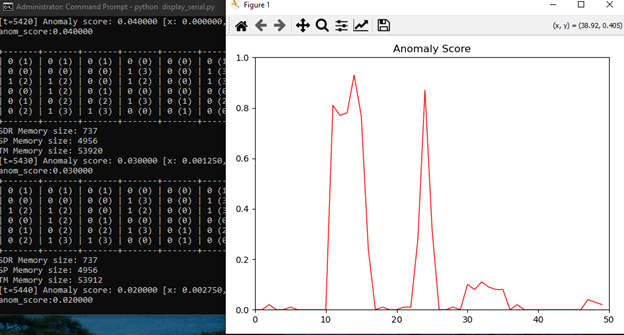
\includegraphics[keepaspectratio]{contents/core/img/chapter8-anomaly-example.png}}

}

\caption{Figure 8.1: Example of IMU Anomaly}

\end{figure}%

\begin{Shaded}
\begin{Highlighting}[]
\NormalTok{sl\_htm\_encoder\_simple\_number}\OperatorTok{(}\NormalTok{imu\_data\_normalized}\OperatorTok{.}\NormalTok{x}\OperatorTok{,} \OperatorTok{{-}}\FloatTok{1.0}\BuiltInTok{f}\OperatorTok{,} \FloatTok{1.0}\BuiltInTok{f}\OperatorTok{,} \DecValTok{9}\OperatorTok{,} \OperatorTok{\&}\NormalTok{sdr\_x}\OperatorTok{);}
\NormalTok{sl\_htm\_encoder\_simple\_number}\OperatorTok{(}\NormalTok{imu\_data\_normalized}\OperatorTok{.}\NormalTok{y}\OperatorTok{,} \OperatorTok{{-}}\FloatTok{1.0}\BuiltInTok{f}\OperatorTok{,} \FloatTok{1.0}\BuiltInTok{f}\OperatorTok{,} \DecValTok{9}\OperatorTok{,} \OperatorTok{\&}\NormalTok{sdr\_y}\OperatorTok{);}
\NormalTok{sl\_htm\_encoder\_simple\_number}\OperatorTok{(}\NormalTok{imu\_data\_normalized}\OperatorTok{.}\NormalTok{z}\OperatorTok{,} \OperatorTok{{-}}\FloatTok{1.0}\BuiltInTok{f}\OperatorTok{,} \FloatTok{1.0}\BuiltInTok{f}\OperatorTok{,} \DecValTok{9}\OperatorTok{,} \OperatorTok{\&}\NormalTok{sdr\_z}\OperatorTok{);}

\NormalTok{sl\_htm\_sdr\_insert}\OperatorTok{(\&}\NormalTok{input\_sdr}\OperatorTok{,} \OperatorTok{\&}\NormalTok{sdr\_x}\OperatorTok{,} \DecValTok{0}\OperatorTok{,}\NormalTok{ SDR\_WIDTH }\OperatorTok{/} \DecValTok{3} \OperatorTok{*} \DecValTok{0}\OperatorTok{);}
\NormalTok{sl\_htm\_sdr\_insert}\OperatorTok{(\&}\NormalTok{input\_sdr}\OperatorTok{,} \OperatorTok{\&}\NormalTok{sdr\_y}\OperatorTok{,} \DecValTok{0}\OperatorTok{,}\NormalTok{ SDR\_WIDTH }\OperatorTok{/} \DecValTok{3} \OperatorTok{*} \DecValTok{1}\OperatorTok{);}
\NormalTok{sl\_htm\_sdr\_insert}\OperatorTok{(\&}\NormalTok{input\_sdr}\OperatorTok{,} \OperatorTok{\&}\NormalTok{sdr\_z}\OperatorTok{,} \DecValTok{0}\OperatorTok{,}\NormalTok{ SDR\_WIDTH }\OperatorTok{/} \DecValTok{3} \OperatorTok{*} \DecValTok{2}\OperatorTok{);}
\end{Highlighting}
\end{Shaded}

\section{Visualization and Real-Time
Monitoring}\label{visualization-and-real-time-monitoring}

The Python script \texttt{display\_serial.py} visualizes anomaly scores
in real-time by reading from a serial port connected to the
microcontroller at a \emph{baudrate=115200}. The script maintains a
rolling buffer of scores and updates a live plot. This script helps
visualize identified anomalies, such as irregular vibrations or sudden
movements.

\begin{Shaded}
\begin{Highlighting}[]
\ControlFlowTok{if}\NormalTok{ line}\OperatorTok{.}\NormalTok{startswith}\OperatorTok{(}\StringTok{"anom\_score"}\OperatorTok{):}
\NormalTok{    line\_info }\OperatorTok{=}\NormalTok{ line}\OperatorTok{.}\NormalTok{split}\OperatorTok{(}\StringTok{":"}\OperatorTok{)}
\NormalTok{    anomaly\_score }\OperatorTok{=} \DataTypeTok{float}\OperatorTok{(}\NormalTok{line\_info}\OperatorTok{[}\DecValTok{1}\OperatorTok{])}
\NormalTok{    buffer}\OperatorTok{.}\NormalTok{append}\OperatorTok{(}\NormalTok{anomaly\_score}\OperatorTok{)}
\NormalTok{    buffer }\OperatorTok{=}\NormalTok{ buffer}\OperatorTok{[}\DecValTok{1}\OperatorTok{:]}
\NormalTok{    axs}\OperatorTok{.}\NormalTok{plot}\OperatorTok{(}\NormalTok{buffer}\OperatorTok{,}\NormalTok{ color}\OperatorTok{=}\StringTok{"red"}\OperatorTok{,}\NormalTok{ linewidth}\OperatorTok{=}\DecValTok{1}\OperatorTok{)}
\NormalTok{    fig}\OperatorTok{.}\NormalTok{tight\_layout}\OperatorTok{()}
\NormalTok{    fig}\OperatorTok{.}\NormalTok{canvas}\OperatorTok{.}\NormalTok{draw}\OperatorTok{()}
\NormalTok{    plt}\OperatorTok{.}\NormalTok{pause}\OperatorTok{(}\FloatTok{0.001}\OperatorTok{)}
\NormalTok{    axs}\OperatorTok{.}\NormalTok{clear}\OperatorTok{()}
\end{Highlighting}
\end{Shaded}

\chapter{\texorpdfstring{\textbf{Audio ML for
EFR32}}{Audio ML for EFR32}}\label{audio-ml-for-efr32}

Implementing audio machine learning (ML) on microcontrollers has become
increasingly common in recent years. Optimizing the model is crucial to
achieve accurate results while maintaining energy efficiency, ensuring
suitability for high-performance embedded systems. This chapter details
the implementation of a basic \emph{Yes/No} audio detection system using
ML. Initially, a neural network is trained to classify two audio
classes: \emph{Yes} and \emph{No}. The trained model is then deployed on
the EFR32 Dev kit.

\section{Overview}\label{overview-1}

In the implementation below, the system processes raw audio input and
categorizes it as either \emph{Yes} or \emph{No} using the trained ML
model. The workflow includes three key stages:

\begin{itemize}
\item
  Training the ML model using TensorFlow.
\item
  Converting the model to a TensorFlow Lite format.
\item
  Deploying the model on the EFR32 MCU for real-time inference.
\end{itemize}

The explanations and code examples are presented below for clarity. The
required concepts are as follows:

\begin{itemize}
\item
  \textbf{TensorFlow:} An open-source framework widely used for
  developing and deploying machine learning models across platforms,
  including mobile and embedded systems. TensorFlow provides tools for
  building, training, and optimizing neural networks, along with
  TensorFlow Lite for Microcontrollers, which allows ML models to run
  efficiently on resource-constrained devices.
\item
  \textbf{Audio Features:} Raw audio data, typically represented as
  waveforms, is transformed into meaningful numerical representations
  suitable for ML models. Commonly used features include Mel Frequency
  Cepstral Coefficients (MFCCs), which capture the spectral properties
  of audio signals, and Spectrograms, which represent the frequency
  content over time. These features enable neural networks to identify
  patterns and classify audio inputs accurately.
\item
  \textbf{Edge ML:} Optimization of ML models for performance and memory
  efficiency on embedded devices.
\end{itemize}

\section{Training the Model in
TensorFlow}\label{training-the-model-in-tensorflow}

\subsection{Preparing the Data}\label{preparing-the-data}

Labeled audio clips containing the words \emph{Yes} and \emph{No} are
required for training a model. A pre-recorded audio dataset, available
in WAV format, will be used in this example. These audio files are first
loaded, processed to extract MFCC features, and splitted into training
and test sets.

\begin{Shaded}
\begin{Highlighting}[]
\NormalTok{import tensorflow as tf}
\NormalTok{import librosa}
\NormalTok{import numpy as np}
\NormalTok{import os}

\PreprocessorTok{\# }\ErrorTok{Extract MFCC features from an audio file}
\NormalTok{def extract\_mfcc}\OperatorTok{(}\NormalTok{file\_path}\OperatorTok{):}
\NormalTok{    y}\OperatorTok{,}\NormalTok{ sr }\OperatorTok{=}\NormalTok{ librosa}\OperatorTok{.}\NormalTok{load}\OperatorTok{(}\NormalTok{file\_path}\OperatorTok{,}\NormalTok{ sr}\OperatorTok{=}\NormalTok{None}\OperatorTok{)}\NormalTok{  \# Load the audio file}
\NormalTok{    mfcc }\OperatorTok{=}\NormalTok{ librosa}\OperatorTok{.}\NormalTok{feature}\OperatorTok{.}\NormalTok{mfcc}\OperatorTok{(}\NormalTok{y}\OperatorTok{=}\NormalTok{y}\OperatorTok{,}\NormalTok{ sr}\OperatorTok{=}\NormalTok{sr}\OperatorTok{,}\NormalTok{ n\_mfcc}\OperatorTok{=}\DecValTok{13}\OperatorTok{)}\NormalTok{  \# Extract MFCCs}
    \ControlFlowTok{return}\NormalTok{ np}\OperatorTok{.}\NormalTok{mean}\OperatorTok{(}\NormalTok{mfcc}\OperatorTok{,}\NormalTok{ axis}\OperatorTok{=}\DecValTok{1}\OperatorTok{)}\NormalTok{  \# Return the average of the MFCCs}


\PreprocessorTok{\# }\ErrorTok{Dataset preparation}
\NormalTok{def prepare\_dataset}\OperatorTok{(}\NormalTok{audio\_dir}\OperatorTok{):}
\NormalTok{    features }\OperatorTok{=} \OperatorTok{[]}
\NormalTok{    labels }\OperatorTok{=} \OperatorTok{[]}
    \ControlFlowTok{for}\NormalTok{ label in }\OperatorTok{[}\CharTok{\textquotesingle{}y}\ErrorTok{es}\CharTok{\textquotesingle{}}\OperatorTok{,} \CharTok{\textquotesingle{}n}\ErrorTok{o}\CharTok{\textquotesingle{}}\OperatorTok{]:}
        \ControlFlowTok{for}\NormalTok{ file in os}\OperatorTok{.}\NormalTok{listdir}\OperatorTok{(}\NormalTok{os}\OperatorTok{.}\NormalTok{path}\OperatorTok{.}\NormalTok{join}\OperatorTok{(}\NormalTok{audio\_dir}\OperatorTok{,}\NormalTok{ label}\OperatorTok{)):}
            \ControlFlowTok{if}\NormalTok{ file}\OperatorTok{.}\NormalTok{endswith}\OperatorTok{(}\CharTok{\textquotesingle{}.}\ErrorTok{wav}\CharTok{\textquotesingle{}}\OperatorTok{):}
\NormalTok{                file\_path }\OperatorTok{=}\NormalTok{ os}\OperatorTok{.}\NormalTok{path}\OperatorTok{.}\NormalTok{join}\OperatorTok{(}\NormalTok{audio\_dir}\OperatorTok{,}\NormalTok{ label}\OperatorTok{,}\NormalTok{ file}\OperatorTok{)}
\NormalTok{                mfcc\_features }\OperatorTok{=}\NormalTok{ extract\_mfcc}\OperatorTok{(}\NormalTok{file\_path}\OperatorTok{)}
\NormalTok{                features}\OperatorTok{.}\NormalTok{append}\OperatorTok{(}\NormalTok{mfcc\_features}\OperatorTok{)}
\NormalTok{                labels}\OperatorTok{.}\NormalTok{append}\OperatorTok{(}\DecValTok{0} \ControlFlowTok{if}\NormalTok{ label }\OperatorTok{==} \CharTok{\textquotesingle{}n}\ErrorTok{o}\CharTok{\textquotesingle{}} \ControlFlowTok{else} \DecValTok{1}\OperatorTok{)}\NormalTok{  \# }\DecValTok{0} \ControlFlowTok{for} \StringTok{"No"}\OperatorTok{,} \DecValTok{1} \ControlFlowTok{for} \StringTok{"Yes"}
    \ControlFlowTok{return}\NormalTok{ np}\OperatorTok{.}\NormalTok{array}\OperatorTok{(}\NormalTok{features}\OperatorTok{),}\NormalTok{ np}\OperatorTok{.}\NormalTok{array}\OperatorTok{(}\NormalTok{labels}\OperatorTok{)}

\NormalTok{X}\OperatorTok{,}\NormalTok{ y }\OperatorTok{=}\NormalTok{ prepare\_dataset}\OperatorTok{(}\CharTok{\textquotesingle{}d}\ErrorTok{ata/audio}\CharTok{\textquotesingle{}}\OperatorTok{)}

\PreprocessorTok{\# }\ErrorTok{Splitting dataset into training and testing sets}
\NormalTok{from sklearn}\OperatorTok{.}\NormalTok{model\_selection import train\_test\_split}
\NormalTok{X\_train}\OperatorTok{,}\NormalTok{ X\_test}\OperatorTok{,}\NormalTok{ y\_train}\OperatorTok{,}\NormalTok{ y\_test }\OperatorTok{=}\NormalTok{ train\_test\_split}\OperatorTok{(}\NormalTok{X}\OperatorTok{,}\NormalTok{ y}\OperatorTok{,}\NormalTok{ test\_size}\OperatorTok{=}\FloatTok{0.2}\OperatorTok{)}
\end{Highlighting}
\end{Shaded}

\subsection{Training the Neural Network
Model}\label{training-the-neural-network-model}

A neural network is defined for binary classification of audio features.

\begin{Shaded}
\begin{Highlighting}[]
\NormalTok{model }\OperatorTok{=}\NormalTok{ tf}\OperatorTok{.}\NormalTok{keras}\OperatorTok{.}\NormalTok{Sequential}\OperatorTok{([}
\NormalTok{    tf}\OperatorTok{.}\NormalTok{keras}\OperatorTok{.}\NormalTok{layers}\OperatorTok{.}\NormalTok{Dense}\OperatorTok{(}\DecValTok{64}\OperatorTok{,}\NormalTok{ activation}\OperatorTok{=}\CharTok{\textquotesingle{}r}\ErrorTok{elu}\CharTok{\textquotesingle{}}\OperatorTok{,}\NormalTok{ input\_shape}\OperatorTok{=(}\DecValTok{13}\OperatorTok{,)),}\NormalTok{  \# }\DecValTok{13}\NormalTok{ MFCC features}
\NormalTok{    tf}\OperatorTok{.}\NormalTok{keras}\OperatorTok{.}\NormalTok{layers}\OperatorTok{.}\NormalTok{Dense}\OperatorTok{(}\DecValTok{32}\OperatorTok{,}\NormalTok{ activation}\OperatorTok{=}\CharTok{\textquotesingle{}r}\ErrorTok{elu}\CharTok{\textquotesingle{}}\OperatorTok{),}
\NormalTok{    tf}\OperatorTok{.}\NormalTok{keras}\OperatorTok{.}\NormalTok{layers}\OperatorTok{.}\NormalTok{Dense}\OperatorTok{(}\DecValTok{1}\OperatorTok{,}\NormalTok{ activation}\OperatorTok{=}\CharTok{\textquotesingle{}s}\ErrorTok{igmoid}\CharTok{\textquotesingle{}}\OperatorTok{)}\NormalTok{  \# Sigmoid }\ControlFlowTok{for}\NormalTok{ binary classification}

\OperatorTok{])}

\NormalTok{model}\OperatorTok{.}\NormalTok{compile}\OperatorTok{(}\NormalTok{optimizer}\OperatorTok{=}\CharTok{\textquotesingle{}a}\ErrorTok{dam}\CharTok{\textquotesingle{}}\OperatorTok{,}\NormalTok{ loss}\OperatorTok{=}\CharTok{\textquotesingle{}b}\ErrorTok{inary\_crossentropy}\CharTok{\textquotesingle{}}\OperatorTok{,}\NormalTok{ metrics}\OperatorTok{=[}\CharTok{\textquotesingle{}a}\ErrorTok{ccuracy}\CharTok{\textquotesingle{}}\OperatorTok{])}
\NormalTok{model}\OperatorTok{.}\NormalTok{fit}\OperatorTok{(}\NormalTok{X\_train}\OperatorTok{,}\NormalTok{ y\_train}\OperatorTok{,}\NormalTok{ epochs}\OperatorTok{=}\DecValTok{10}\OperatorTok{,}\NormalTok{ batch\_size}\OperatorTok{=}\DecValTok{32}\OperatorTok{,}\NormalTok{ validation\_data}\OperatorTok{=(}\NormalTok{X\_test}\OperatorTok{,}\NormalTok{ y\_test}\OperatorTok{))}

\PreprocessorTok{\# }\ErrorTok{Save the trained model}
\NormalTok{model}\OperatorTok{.}\NormalTok{save}\OperatorTok{(}\CharTok{\textquotesingle{}y}\ErrorTok{es\_no\_model.h5}\CharTok{\textquotesingle{}}\OperatorTok{)}
\end{Highlighting}
\end{Shaded}

\section{Converting the Model for MCU
Deployment}\label{converting-the-model-for-mcu-deployment}

The trained TensorFlow model is converted into TensorFlow Lite (TFLite)
format for efficient deployment on resource-constrained devices.

\begin{Shaded}
\begin{Highlighting}[]
\NormalTok{model }\OperatorTok{=}\NormalTok{ tf}\OperatorTok{.}\NormalTok{keras}\OperatorTok{.}\NormalTok{models}\OperatorTok{.}\NormalTok{load\_model}\OperatorTok{(}\CharTok{\textquotesingle{}y}\ErrorTok{es\_no\_model.h5}\CharTok{\textquotesingle{}}\OperatorTok{)}
\NormalTok{converter }\OperatorTok{=}\NormalTok{ tf}\OperatorTok{.}\NormalTok{lite}\OperatorTok{.}\NormalTok{TFLiteConverter}\OperatorTok{.}\NormalTok{from\_keras\_model}\OperatorTok{(}\NormalTok{model}\OperatorTok{)}
\NormalTok{tflite\_model }\OperatorTok{=}\NormalTok{ converter}\OperatorTok{.}\NormalTok{convert}\OperatorTok{()}

\PreprocessorTok{\# }\ErrorTok{Save the TensorFlow Lite model}
\NormalTok{with open}\OperatorTok{(}\CharTok{\textquotesingle{}y}\ErrorTok{es\_no\_model.tflite}\CharTok{\textquotesingle{}}\OperatorTok{,} \CharTok{\textquotesingle{}w}\ErrorTok{b}\CharTok{\textquotesingle{}}\OperatorTok{)}\NormalTok{ as f}\OperatorTok{:}
\NormalTok{    f}\OperatorTok{.}\NormalTok{write}\OperatorTok{(}\NormalTok{tflite\_model}\OperatorTok{)}
\end{Highlighting}
\end{Shaded}

The conversion produces a `.tflite' file suitable for embedded
deployment.

\section{Implementing the Model on the
EFR32xG24}\label{implementing-the-model-on-the-efr32xg24}

The TensorFlow Lite model is integrated into the EFR32xG24 environment
using the appropriate software development kit (SDK) and TensorFlow Lite
for Microcontrollers library.

\subsection{Setting Up the Development
Environment}\label{setting-up-the-development-environment}

The following components are required for setting up the development
environment:

\begin{itemize}
\item
  \textbf{EFR32xG24 SDK:} The latest version of the Silicon Labs Gecko
  SDK must be installed.
\item
  \textbf{TensorFlow Lite for Microcontrollers:} This library should be
  set up within the development environment.
\end{itemize}

\subsection{Loading the Model and Running
Inference}\label{loading-the-model-and-running-inference}

The TensorFlow Lite model is loaded onto the MCU, input data is
prepared, and inference is performed.

\begin{Shaded}
\begin{Highlighting}[]
\PreprocessorTok{\#include }\ImportTok{"tensorflow/lite/c/common.h"}
\PreprocessorTok{\#include }\ImportTok{"tensorflow/lite/micro/micro\_interpreter.h"}
\PreprocessorTok{\#include }\ImportTok{"tensorflow/lite/model.h"}
\PreprocessorTok{\#include }\ImportTok{"tensorflow/lite/schema/schema\_generated.h"}
\PreprocessorTok{\#include }\ImportTok{"tensorflow/lite/kernels/register.h"}

\PreprocessorTok{\#define INPUT\_SIZE }\DecValTok{13}

\CommentTok{// Declare tensors and interpreter}
\NormalTok{tflite}\OperatorTok{::}\NormalTok{MicroInterpreter}\OperatorTok{*}\NormalTok{ interpreter}\OperatorTok{;}
\NormalTok{tflite}\OperatorTok{::}\NormalTok{Model}\OperatorTok{*}\NormalTok{ model}\OperatorTok{;}
\NormalTok{tflite}\OperatorTok{::}\NormalTok{MicroAllocator}\OperatorTok{*}\NormalTok{ allocator}\OperatorTok{;}

\DataTypeTok{float}\NormalTok{ input\_data}\OperatorTok{[}\NormalTok{INPUT\_SIZE}\OperatorTok{];}  \CommentTok{// Input data (MFCCs)}
\DataTypeTok{float}\NormalTok{ output\_data}\OperatorTok{[}\DecValTok{1}\OperatorTok{];}  \CommentTok{// Output data (prediction)}


\CommentTok{// Load the TensorFlow Lite model}
\DataTypeTok{void}\NormalTok{ LoadModel}\OperatorTok{(}\DataTypeTok{const} \DataTypeTok{uint8\_t}\OperatorTok{*}\NormalTok{ model\_data}\OperatorTok{)} \OperatorTok{\{}
\NormalTok{    model }\OperatorTok{=}\NormalTok{ tflite}\OperatorTok{::}\NormalTok{GetModel}\OperatorTok{(}\NormalTok{model\_data}\OperatorTok{);}
\NormalTok{    tflite}\OperatorTok{::}\NormalTok{ops}\OperatorTok{::}\NormalTok{micro}\OperatorTok{::}\NormalTok{RegisterAllOps}\OperatorTok{();}
\NormalTok{    tflite}\OperatorTok{::}\NormalTok{MicroInterpreter interpreter}\OperatorTok{(}\NormalTok{model}\OperatorTok{,}\NormalTok{ tensor\_arena}\OperatorTok{,}\NormalTok{ kTensorArenaSize}\OperatorTok{,} \OperatorTok{\&}\NormalTok{resolver}\OperatorTok{,} \OperatorTok{\&}\NormalTok{allocator}\OperatorTok{);}
\NormalTok{    interpreter}\OperatorTok{.}\NormalTok{AllocateTensors}\OperatorTok{();}
\OperatorTok{\}}

\CommentTok{// Perform audio classification}
\DataTypeTok{int}\NormalTok{ ClassifyAudio}\OperatorTok{(}\DataTypeTok{float}\OperatorTok{*}\NormalTok{ mfcc\_input}\OperatorTok{)} \OperatorTok{\{}
    \CommentTok{// Copy MFCC data into the input tensor}
\NormalTok{    memcpy}\OperatorTok{(}\NormalTok{interpreter}\OperatorTok{.}\NormalTok{input}\OperatorTok{(}\DecValTok{0}\OperatorTok{){-}\textgreater{}}\NormalTok{data}\OperatorTok{.}\NormalTok{f}\OperatorTok{,}\NormalTok{ mfcc\_input}\OperatorTok{,} \KeywordTok{sizeof}\OperatorTok{(}\DataTypeTok{float}\OperatorTok{)} \OperatorTok{*}\NormalTok{ INPUT\_SIZE}\OperatorTok{);}
    
    \CommentTok{// Perform inference}
\NormalTok{    interpreter}\OperatorTok{.}\NormalTok{Invoke}\OperatorTok{();}

    \CommentTok{// Get the output prediction}
    \DataTypeTok{float}\NormalTok{ prediction }\OperatorTok{=}\NormalTok{ interpreter}\OperatorTok{.}\NormalTok{output}\OperatorTok{(}\DecValTok{0}\OperatorTok{){-}\textgreater{}}\NormalTok{data}\OperatorTok{.}\NormalTok{f}\OperatorTok{[}\DecValTok{0}\OperatorTok{];}

    \CommentTok{// Return classification result: 1 for "Yes", 0 for "No"}
    \ControlFlowTok{return}\NormalTok{ prediction }\OperatorTok{\textgreater{}} \FloatTok{0.5} \OperatorTok{?} \DecValTok{1} \OperatorTok{:} \DecValTok{0}\OperatorTok{;}

\OperatorTok{\}}
\end{Highlighting}
\end{Shaded}

The inference results are interpreted as:

\begin{itemize}
\item
  1: Detected \emph{Yes}
\item
  0: Detected \emph{No}
\end{itemize}

\subsection{Integrating Audio Capture}\label{integrating-audio-capture}

An onboard microphone or an external microphone is often used to
interface with the MCU to process real-time audio input. The EFR32xG24
does not include a dedicated audio processing block, requiring
integration with a microphone module that outputs either analog signals
(such as those from an electret microphone) or digital signals (like
those from an I2S microphone). For simplicity, an analog microphone with
an ADC on the MCU is employed here, with audio signals sampled,
preprocessed, and then classified using the following steps:

\begin{enumerate}
\def\labelenumi{\arabic{enumi}.}
\item
  Configure the ADC to sample audio signals.
\item
  Capture the raw samples from the ADC at a suitable rate (e.g., 16 kHz
  or 8 kHz, depending on requirements).
\item
  Preprocess the audio to extract features such as MFCC (Mel-frequency
  cepstral coefficients), which are suitable for ML models.
\item
  Feed these features into the model for classification.
\end{enumerate}

Here is an example of how to collect and process audio data using an ADC
for feature extraction using the EFR32 SDK.

\begin{Shaded}
\begin{Highlighting}[]
\PreprocessorTok{\#include }\ImportTok{"em\_device.h"}
\PreprocessorTok{\#include }\ImportTok{"em\_chip.h"}
\PreprocessorTok{\#include }\ImportTok{"em\_adc.h"}
\PreprocessorTok{\#include }\ImportTok{"em\_cmu.h"}
\PreprocessorTok{\#include }\ImportTok{"em\_gpio.h"}
\PreprocessorTok{\#include }\ImportTok{"em\_interrupt.h"}

\CommentTok{// ADC buffer for storing captured samples}
\PreprocessorTok{\#define BUFFER\_SIZE }\DecValTok{1024}
\DataTypeTok{static} \DataTypeTok{uint16\_t}\NormalTok{ adc\_buffer}\OperatorTok{[}\NormalTok{BUFFER\_SIZE}\OperatorTok{];}
\DataTypeTok{static} \DataTypeTok{volatile} \DataTypeTok{uint32\_t}\NormalTok{ adc\_index }\OperatorTok{=} \DecValTok{0}\OperatorTok{;}  \CommentTok{// Index for storing samples in the buffer}

\CommentTok{// ADC interrupt handler to collect samples}
\DataTypeTok{void}\NormalTok{ ADC0\_IRQHandler}\OperatorTok{(}\DataTypeTok{void}\OperatorTok{)} \OperatorTok{\{}
    \CommentTok{// Read the ADC data from the ADC data register}
\NormalTok{    adc\_buffer}\OperatorTok{[}\NormalTok{adc\_index}\OperatorTok{++]} \OperatorTok{=}\NormalTok{ ADC\_DataSingleGet}\OperatorTok{(}\NormalTok{ADC0}\OperatorTok{);}

    \CommentTok{// If the buffer is full, stop the ADC conversion}
    \ControlFlowTok{if} \OperatorTok{(}\NormalTok{adc\_index }\OperatorTok{\textgreater{}=}\NormalTok{ BUFFER\_SIZE}\OperatorTok{)} \OperatorTok{\{}
\NormalTok{        ADC0}\OperatorTok{{-}\textgreater{}}\NormalTok{CMD }\OperatorTok{=}\NormalTok{ ADC\_CMD\_STOP}\OperatorTok{;}
\NormalTok{        adc\_index }\OperatorTok{=} \DecValTok{0}\OperatorTok{;}
    \OperatorTok{\}}
\OperatorTok{\}}

\CommentTok{// Initialize the ADC for audio sampling}
\DataTypeTok{void}\NormalTok{ ADC\_InitAudio}\OperatorTok{(}\DataTypeTok{void}\OperatorTok{)} \OperatorTok{\{}
    \CommentTok{// Enable the clock for ADC and GPIO}
\NormalTok{    CMU\_ClockEnable}\OperatorTok{(}\NormalTok{cmuClock\_ADC0}\OperatorTok{,} \KeywordTok{true}\OperatorTok{);}
\NormalTok{    CMU\_ClockEnable}\OperatorTok{(}\NormalTok{cmuClock\_GPIO}\OperatorTok{,} \KeywordTok{true}\OperatorTok{);}

    \CommentTok{// Configure the GPIO pin for the microphone (assuming it is connected to a pin, e.g., PA0)}
\NormalTok{    GPIO\_PinModeSet}\OperatorTok{(}\NormalTok{gpioPortA}\OperatorTok{,} \DecValTok{0}\OperatorTok{,}\NormalTok{ gpioModeInput}\OperatorTok{,} \DecValTok{0}\OperatorTok{);}

    \CommentTok{// Configure the ADC to sample at a reasonable rate for audio (e.g., 16 kHz)}
\NormalTok{    ADC\_Init\_TypeDef adcInit }\OperatorTok{=}\NormalTok{ ADC\_INIT\_DEFAULT}\OperatorTok{;}
\NormalTok{    adcInit}\OperatorTok{.}\NormalTok{prescale }\OperatorTok{=}\NormalTok{ ADC\_PrescaleCalc}\OperatorTok{(}\DecValTok{16000}\OperatorTok{,} \DecValTok{0}\OperatorTok{);}  \CommentTok{// Calculate prescaler for 16kHz sampling rate}
\NormalTok{    ADC\_Init}\OperatorTok{(}\NormalTok{ADC0}\OperatorTok{,} \OperatorTok{\&}\NormalTok{adcInit}\OperatorTok{);}

    \CommentTok{// Configure the ADC single conversion mode}
\NormalTok{    ADC\_InitSingle\_TypeDef adcSingleInit }\OperatorTok{=}\NormalTok{ ADC\_INITSINGLE\_DEFAULT}\OperatorTok{;}
\NormalTok{    adcSingleInit}\OperatorTok{.}\NormalTok{input }\OperatorTok{=}\NormalTok{ adcSingleInputPin0}\OperatorTok{;}  \CommentTok{// Set the input channel (e.g., PA0)}
\NormalTok{    adcSingleInit}\OperatorTok{.}\NormalTok{acqTime }\OperatorTok{=}\NormalTok{ adcAcqTime4}\OperatorTok{;}       \CommentTok{// Set acquisition time}
\NormalTok{    ADC\_InitSingle}\OperatorTok{(}\NormalTok{ADC0}\OperatorTok{,} \OperatorTok{\&}\NormalTok{adcSingleInit}\OperatorTok{);}

    \CommentTok{// Enable the ADC interrupt and start ADC conversions}
\NormalTok{    NVIC\_EnableIRQ}\OperatorTok{(}\NormalTok{ADC0\_IRQn}\OperatorTok{);}
\NormalTok{    ADC0}\OperatorTok{{-}\textgreater{}}\NormalTok{CMD }\OperatorTok{=}\NormalTok{ ADC\_CMD\_START}\OperatorTok{;}
\OperatorTok{\}}
\end{Highlighting}
\end{Shaded}

\subsection{Audio Preprocessing and
Classification}\label{audio-preprocessing-and-classification}

The audio data is stored in an array adc\_buffer where the ADC samples
are placed at regular intervals following these steps:

\begin{itemize}
\item
  ADC samples the microphone data at a fixed rate.
\item
  The interrupt service routine (ISR) will be triggered each time the
  ADC completes a conversion.
\item
  The ISR stores the data into the adc\_buffer.
\end{itemize}

Once the raw ADC samples are in the buffer, preprocessing is needed for
the ML model. An example is as follows:

\begin{itemize}
\item
  Convert the ADC samples to a window of audio (e.g., 25 ms).
\item
  Apply a Fourier transform to convert the time-domain signal to the
  frequency domain.
\item
  Extract MFCC features from the frequency-domain signal.
\end{itemize}

An example is provided on how to use the buffer data to classify using a
Tensorflow Lite model.

\begin{Shaded}
\begin{Highlighting}[]
\DataTypeTok{void}\NormalTok{ ProcessAudioAndClassify}\OperatorTok{()} \OperatorTok{\{}
    \CommentTok{// Preprocess the raw ADC samples (simplified; actual MFCC extraction would be more complex)}
    \DataTypeTok{float}\NormalTok{ mfcc\_input}\OperatorTok{[}\NormalTok{INPUT\_SIZE}\OperatorTok{];}  \CommentTok{// Assumed 13 MFCC features}
    
    \CommentTok{// For simplicity, the ADC data is copied directly into the input array}
    \CommentTok{// In a real case, processing is required (e.g., via FFT and MFCC extraction)}

    \DataTypeTok{float}\NormalTok{ mfcc\_input}\OperatorTok{[}\NormalTok{INPUT\_SIZE}\OperatorTok{];}
    \ControlFlowTok{for} \OperatorTok{(}\DataTypeTok{int}\NormalTok{ i }\OperatorTok{=} \DecValTok{0}\OperatorTok{;}\NormalTok{ i }\OperatorTok{\textless{}}\NormalTok{ INPUT\_SIZE}\OperatorTok{;}\NormalTok{ i}\OperatorTok{++)} \OperatorTok{\{}
\NormalTok{        mfcc\_input}\OperatorTok{[}\NormalTok{i}\OperatorTok{]} \OperatorTok{=} \OperatorTok{(}\DataTypeTok{float}\OperatorTok{)}\NormalTok{adc\_buffer}\OperatorTok{[}\NormalTok{i}\OperatorTok{];}
    \OperatorTok{\}}

    \CommentTok{// Run the model to classify the audio}
    \DataTypeTok{int}\NormalTok{ prediction }\OperatorTok{=}\NormalTok{ ClassifyAudio}\OperatorTok{(}\NormalTok{mfcc\_input}\OperatorTok{);}
    \ControlFlowTok{if} \OperatorTok{(}\NormalTok{prediction }\OperatorTok{==} \DecValTok{1}\OperatorTok{)} \OperatorTok{\{}
\NormalTok{        printf}\OperatorTok{(}\StringTok{"Detected: Yes}\SpecialCharTok{\textbackslash{}n}\StringTok{"}\OperatorTok{);}
    \OperatorTok{\}} \ControlFlowTok{else} \OperatorTok{\{}
\NormalTok{        printf}\OperatorTok{(}\StringTok{"Detected: No}\SpecialCharTok{\textbackslash{}n}\StringTok{"}\OperatorTok{);}
    \OperatorTok{\}}
\OperatorTok{\}}
\end{Highlighting}
\end{Shaded}

The main loop manages continuous audio capture and classification.

\begin{Shaded}
\begin{Highlighting}[]
\DataTypeTok{int}\NormalTok{ main}\OperatorTok{(}\DataTypeTok{void}\OperatorTok{)} \OperatorTok{\{}
\NormalTok{    CHIP\_Init}\OperatorTok{();}
\NormalTok{    ADC\_InitAudio}\OperatorTok{();}

    \ControlFlowTok{while} \OperatorTok{(}\DecValTok{1}\OperatorTok{)} \OperatorTok{\{}
\NormalTok{        ProcessAudioAndClassify}\OperatorTok{();}
\NormalTok{        EMU\_EnterEM1}\OperatorTok{();}
    \OperatorTok{\}}
\OperatorTok{\}}
\end{Highlighting}
\end{Shaded}

\subsection{Considerations for
Optimization}\label{considerations-for-optimization}

\begin{itemize}
\item
  \textbf{ADC Resolution:} The ADC resolution and sampling rate must
  align with audio requirements.
\item
  \textbf{MFCC Extraction:} Complex preprocessing, such as Fourier
  Transform and MFCC extraction, may require optimizations.
\item
  \textbf{Performance:} Model complexity and sampling rates should be
  adjusted for available memory and processing capabilities.
\end{itemize}


\backmatter


\end{document}
